\chapter{View}
\begin{figure}[!hbp]
	\centering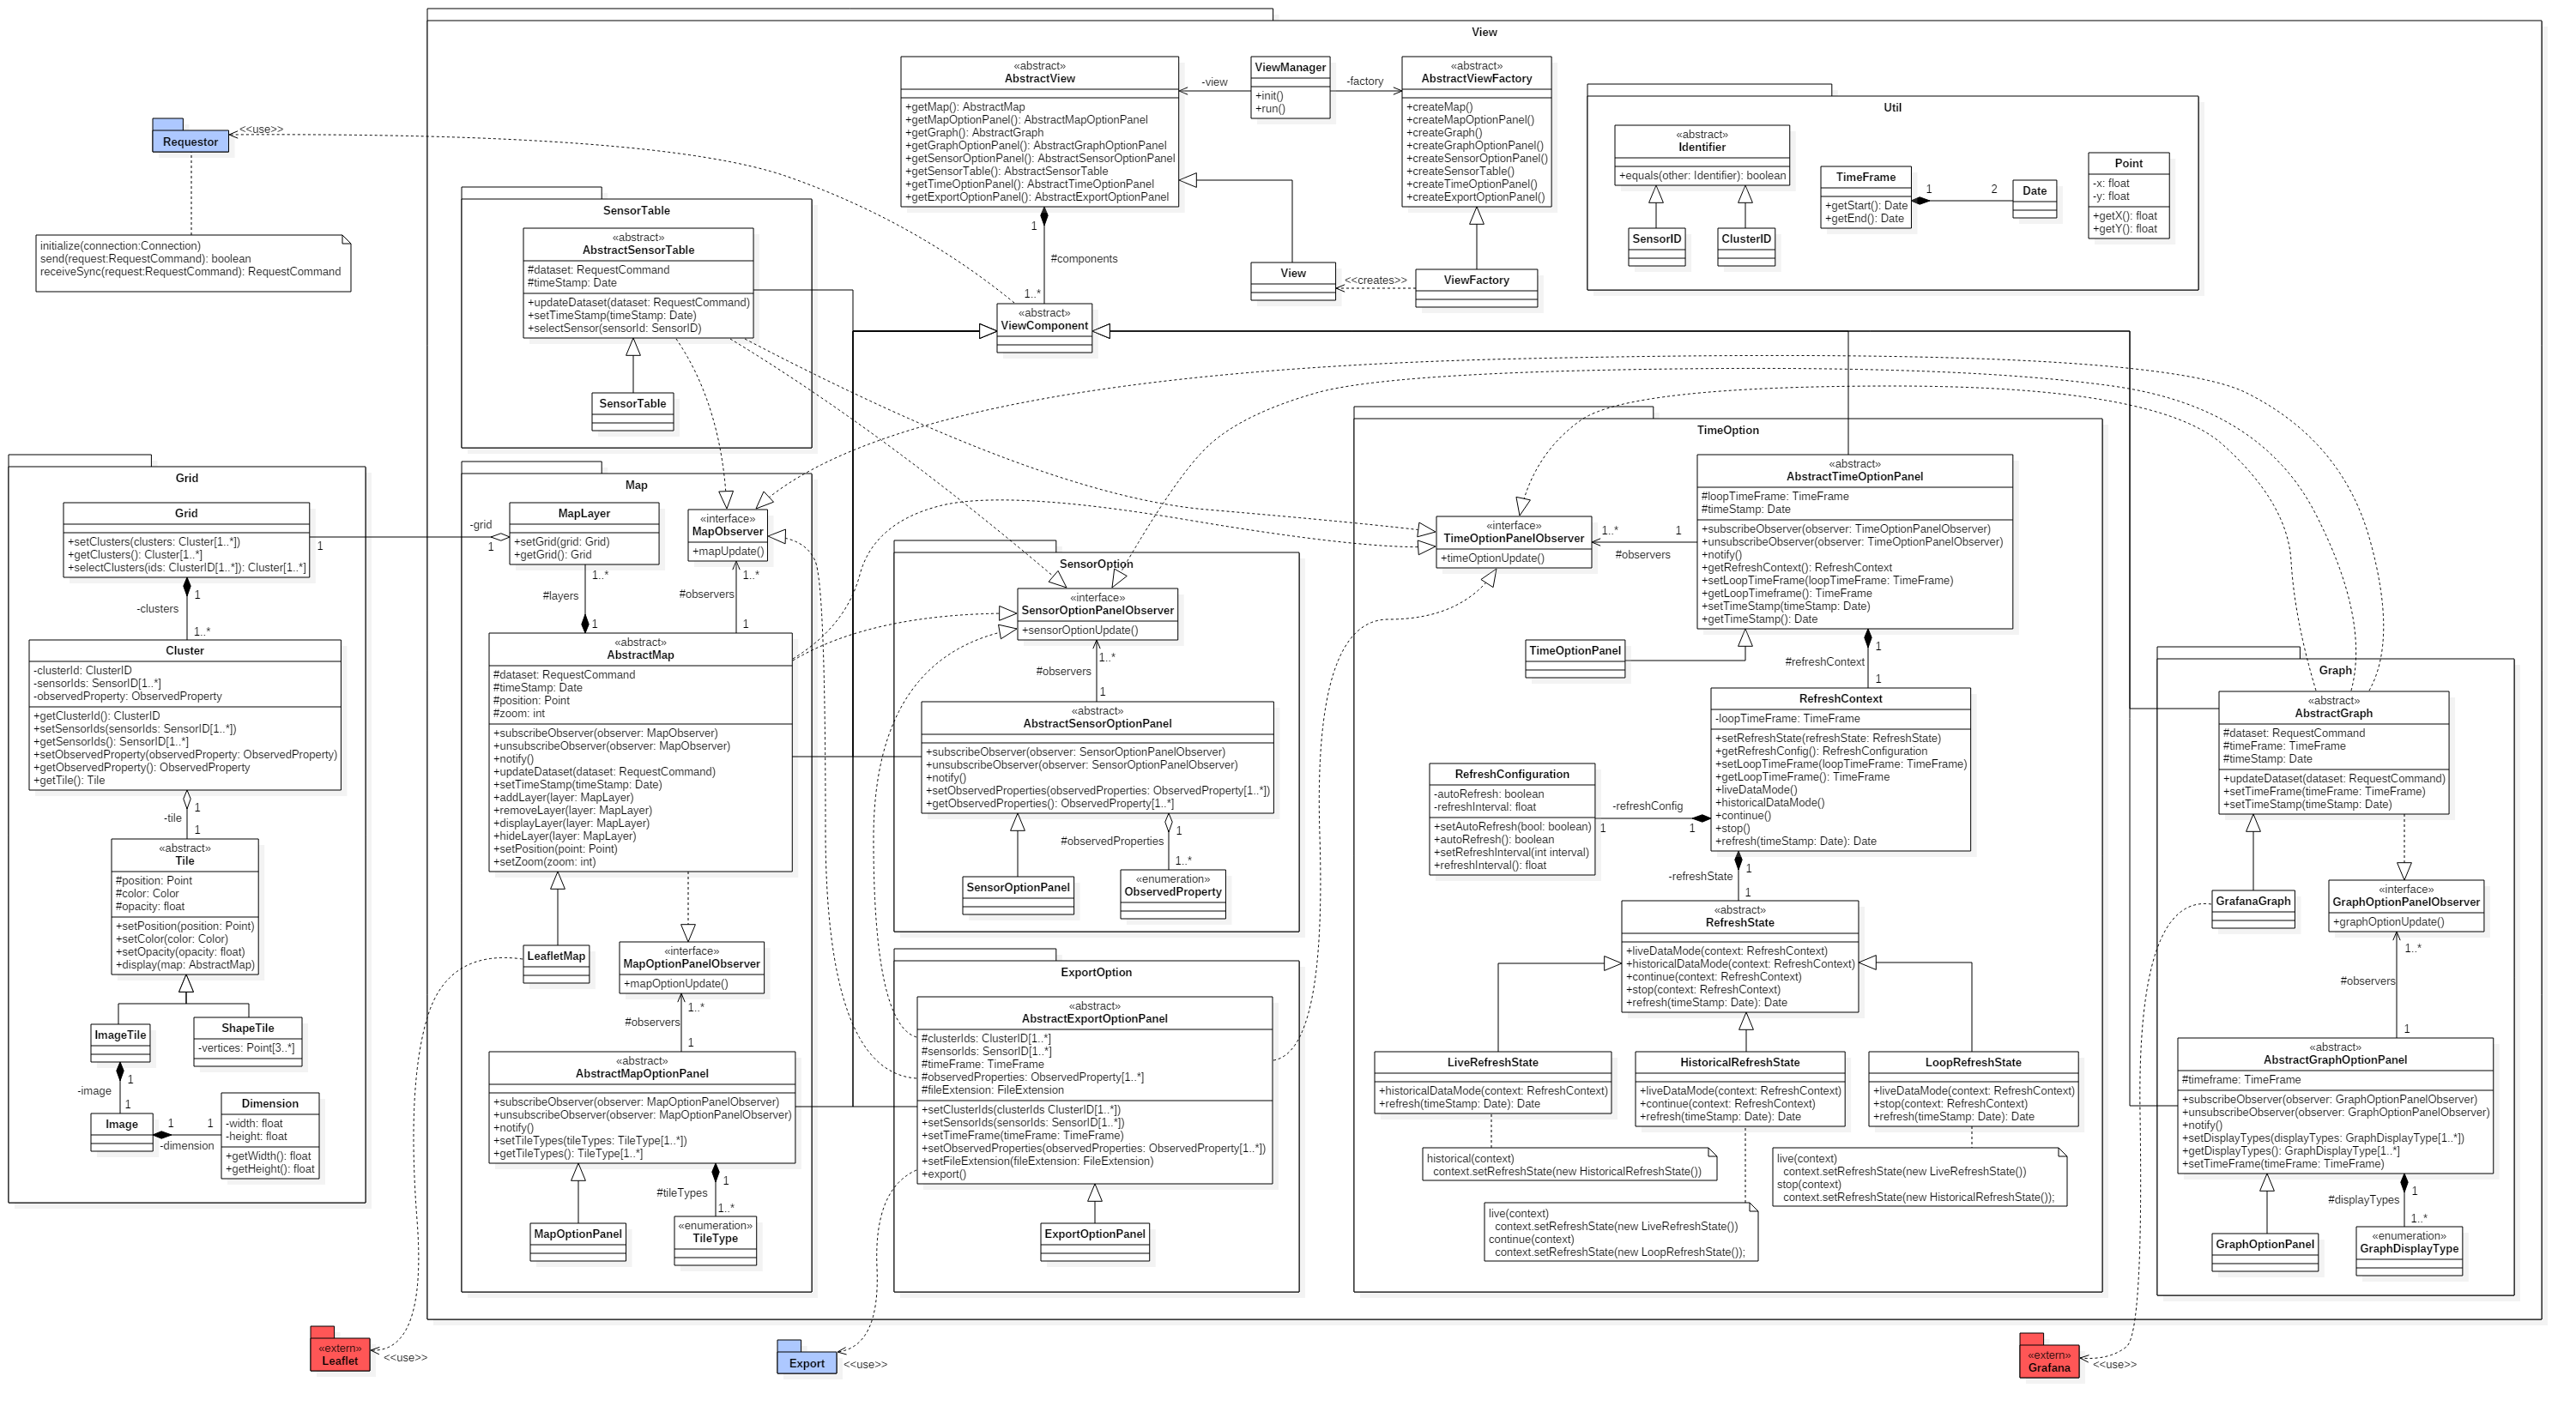
\includegraphics[width=1.25\linewidth,angle=90]{images/view/ViewClassDiagram}
	\caption{Klassendiagramm View}
\end{figure}
\section{Package Grid}{
\label{Grid}\hypertarget{Grid}{}
\hskip -.05in
\hbox to \hsize{\textit{ Package Contents\hfil Page}}
\vskip .13in
\hbox{{\bf  Classes}}
\entityintro{Cluster}{Grid.Cluster}{Encapsulates multiple sensors into a single object by using their specific SensorIDs and provides a graphical representation of their values average by using a Tile.}
\entityintro{Dimension}{Grid.Dimension}{Encapsulates the width and height of a component in float precision.}
\entityintro{Grid}{Grid.Grid}{Encapsulates multiple Clusters into a single object.}
\entityintro{Image}{Grid.Image}{Represents a graphical image.}
\entityintro{ImageTile}{Grid.ImageTile}{A Tile whose graphical representation consists of an image.}
\entityintro{ShapeTile}{Grid.ShapeTile}{A Tile whose graphical representation consists of a shape, specified by an array of vertices.}
\entityintro{Tile}{Grid.Tile}{A graphical structure that can be displayed on an AbstractMap.}
\vskip .1in
\vskip .1in
\newpage
\subsection{\label{Grid.Cluster}Class Cluster}{
\hypertarget{Grid.Cluster}{}\vskip .1in 
Encapsulates multiple sensors into a single object by using their specific SensorIDs and provides a graphical representation of their values average by using a Tile.\vskip .1in
\begin{figure}[!hbp]
	\centering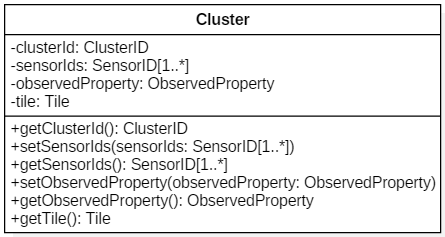
\includegraphics[width=0.5\linewidth]{images/view/classes/Cluster}
\end{figure} 
\subsubsection{Declaration}{
\begin{lstlisting}[frame=none]
public class Cluster
 extends java.lang.Object\end{lstlisting}
\subsubsection{Constructor summary}{
\begin{verse}
\hyperlink{Grid.Cluster()}{{\bf Cluster()}} Default constructor\\
\end{verse}
}
\subsubsection{Method summary}{
\begin{verse}
\hyperlink{Grid.Cluster.getClusterId()}{{\bf getClusterId()}} Get the ClusterID of this Cluster.\\
\hyperlink{Grid.Cluster.getObservedProperty()}{{\bf getObservedProperty()}} Get the ObservedProperty of this Cluster.\\
\hyperlink{Grid.Cluster.getSensorIds()}{{\bf getSensorIds()}} Get all SensorIDs of the sensors contained in this cluster.\\
\hyperlink{Grid.Cluster.getTile()}{{\bf getTile()}} Get the Tile of this Cluster.\\
\hyperlink{Grid.Cluster.setObservedProperty(ObservedProperty)}{{\bf setObservedProperty(ObservedProperty)}} Set the ObservedProperty of this Cluster.\\
\hyperlink{Grid.Cluster.setSensorIds(java.util.Set)}{{\bf setSensorIds(Set)}} Set the SensorIDs of the sensors contained in this cluster.\\
\end{verse}
}
\subsubsection{Constructors}{
\vskip -2em
\begin{itemize}
\item{ 
\index{Cluster()}
\hypertarget{Grid.Cluster()}{{\bf  Cluster}\\}
\begin{lstlisting}[frame=none]
public Cluster()\end{lstlisting} %end signature
\begin{itemize}
\item{
{\bf  Description}

Default constructor
}
\end{itemize}
}%end item
\end{itemize}
}
\subsubsection{Methods}{
\vskip -2em
\begin{itemize}
\item{ 
\index{getClusterId()}
\hypertarget{Grid.Cluster.getClusterId()}{{\bf  getClusterId}\\}
\begin{lstlisting}[frame=none]
public ClusterID getClusterId()\end{lstlisting} %end signature
\begin{itemize}
\item{
{\bf  Description}

Get the ClusterID of this Cluster.
}
\item{{\bf  Returns} -- 
the ClusterID of this Cluster. 
}%end item
\end{itemize}
}%end item
\item{ 
\index{getObservedProperty()}
\hypertarget{Grid.Cluster.getObservedProperty()}{{\bf  getObservedProperty}\\}
\begin{lstlisting}[frame=none]
public ObservedProperty getObservedProperty()\end{lstlisting} %end signature
\begin{itemize}
\item{
{\bf  Description}

Get the ObservedProperty of this Cluster.
}
\item{{\bf  Returns} -- 
the ObservedProperty of this Cluster. 
}%end item
\end{itemize}
}%end item
\item{ 
\index{getSensorIds()}
\hypertarget{Grid.Cluster.getSensorIds()}{{\bf  getSensorIds}\\}
\begin{lstlisting}[frame=none]
public java.util.Set getSensorIds()\end{lstlisting} %end signature
\begin{itemize}
\item{
{\bf  Description}

Get all SensorIDs of the sensors contained in this cluster.
}
\item{{\bf  Returns} -- 
all SensorIDs of the sensors contained in this cluster. 
}%end item
\end{itemize}
}%end item
\item{ 
\index{getTile()}
\hypertarget{Grid.Cluster.getTile()}{{\bf  getTile}\\}
\begin{lstlisting}[frame=none]
public Tile getTile()\end{lstlisting} %end signature
\begin{itemize}
\item{
{\bf  Description}

Get the Tile of this Cluster.
}
\item{{\bf  Returns} -- 
the Tile of this Cluster. 
}%end item
\end{itemize}
}%end item
\item{ 
\index{setObservedProperty(ObservedProperty)}
\hypertarget{Grid.Cluster.setObservedProperty(ObservedProperty)}{{\bf  setObservedProperty}\\}
\begin{lstlisting}[frame=none]
public void setObservedProperty(ObservedProperty observedProperty)\end{lstlisting} %end signature
\begin{itemize}
\item{
{\bf  Description}

Set the ObservedProperty of this Cluster.
}
\item{
{\bf  Parameters}
  \begin{itemize}
   \item{
\texttt{observedProperty} -- }
  \end{itemize}
}%end item
\end{itemize}
}%end item
\item{ 
\index{setSensorIds(Set)}
\hypertarget{Grid.Cluster.setSensorIds(java.util.Set)}{{\bf  setSensorIds}\\}
\begin{lstlisting}[frame=none]
public void setSensorIds(java.util.Set sensorIds)\end{lstlisting} %end signature
\begin{itemize}
\item{
{\bf  Description}

Set the SensorIDs of the sensors contained in this cluster.
}
\item{
{\bf  Parameters}
  \begin{itemize}
   \item{
\texttt{sensorIds} -- }
  \end{itemize}
}%end item
\end{itemize}
}%end item
\end{itemize}
}
}
\subsection{\label{Grid.Dimension}Class Dimension}{
\hypertarget{Grid.Dimension}{}\vskip .1in 
Encapsulates the width and height of a component in float precision.\vskip .1in
\begin{figure}[!hbp]
	\centering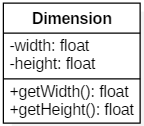
\includegraphics[width=0.5\linewidth]{images/view/classes/Dimension}
\end{figure} 
\subsubsection{Declaration}{
\begin{lstlisting}[frame=none]
public class Dimension
 extends java.lang.Object\end{lstlisting}
\subsubsection{Constructor summary}{
\begin{verse}
\hyperlink{Grid.Dimension()}{{\bf Dimension()}} Default constructor\\
\end{verse}
}
\subsubsection{Method summary}{
\begin{verse}
\hyperlink{Grid.Dimension.getHeight()}{{\bf getHeight()}} Get the height of this Dimension.\\
\hyperlink{Grid.Dimension.getWidth()}{{\bf getWidth()}} Get the width of this Dimension.\\
\end{verse}
}
\subsubsection{Constructors}{
\vskip -2em
\begin{itemize}
\item{ 
\index{Dimension()}
\hypertarget{Grid.Dimension()}{{\bf  Dimension}\\}
\begin{lstlisting}[frame=none]
public Dimension()\end{lstlisting} %end signature
\begin{itemize}
\item{
{\bf  Description}

Default constructor
}
\end{itemize}
}%end item
\end{itemize}
}
\subsubsection{Methods}{
\vskip -2em
\begin{itemize}
\item{ 
\index{getHeight()}
\hypertarget{Grid.Dimension.getHeight()}{{\bf  getHeight}\\}
\begin{lstlisting}[frame=none]
public float getHeight()\end{lstlisting} %end signature
\begin{itemize}
\item{
{\bf  Description}

Get the height of this Dimension.
}
\item{{\bf  Returns} -- 
the height of this Dimension. 
}%end item
\end{itemize}
}%end item
\item{ 
\index{getWidth()}
\hypertarget{Grid.Dimension.getWidth()}{{\bf  getWidth}\\}
\begin{lstlisting}[frame=none]
public float getWidth()\end{lstlisting} %end signature
\begin{itemize}
\item{
{\bf  Description}

Get the width of this Dimension.
}
\item{{\bf  Returns} -- 
the width of this Dimension. 
}%end item
\end{itemize}
}%end item
\end{itemize}
}
}
\subsection{\label{Grid.Grid}Class Grid}{
\hypertarget{Grid.Grid}{}\vskip .1in 
Encapsulates multiple Clusters into a single object.\vskip .1in 
\begin{figure}[!hbp]
	\centering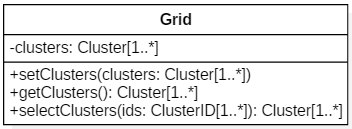
\includegraphics[width=0.5\linewidth]{images/view/classes/Grid}
\end{figure} 
\subsubsection{Declaration}{
\begin{lstlisting}[frame=none]
public class Grid
 extends java.lang.Object\end{lstlisting}
\subsubsection{Constructor summary}{
\begin{verse}
\hyperlink{Grid.Grid()}{{\bf Grid()}} Default constructor\\
\end{verse}
}
\subsubsection{Method summary}{
\begin{verse}
\hyperlink{Grid.Grid.getClusters()}{{\bf getClusters()}} Get all Clusters contained in this Grid.\\
\hyperlink{Grid.Grid.selectClusters(java.util.Set)}{{\bf selectClusters(Set)}} Select Clusters contained in this Grid by using their specific ClusterIDs.\\
\hyperlink{Grid.Grid.setClusters(java.util.Set)}{{\bf setClusters(Set)}} Set the Clusters contained in this Grid.\\
\end{verse}
}
\subsubsection{Constructors}{
\vskip -2em
\begin{itemize}
\item{ 
\index{Grid()}
\hypertarget{Grid.Grid()}{{\bf  Grid}\\}
\begin{lstlisting}[frame=none]
public Grid()\end{lstlisting} %end signature
\begin{itemize}
\item{
{\bf  Description}

Default constructor
}
\end{itemize}
}%end item
\end{itemize}
}
\subsubsection{Methods}{
\vskip -2em
\begin{itemize}
\item{ 
\index{getClusters()}
\hypertarget{Grid.Grid.getClusters()}{{\bf  getClusters}\\}
\begin{lstlisting}[frame=none]
public java.util.Set getClusters()\end{lstlisting} %end signature
\begin{itemize}
\item{
{\bf  Description}

Get all Clusters contained in this Grid.
}
\item{{\bf  Returns} -- 
all Clusters contained in this Grid. 
}%end item
\end{itemize}
}%end item
\item{ 
\index{selectClusters(Set)}
\hypertarget{Grid.Grid.selectClusters(java.util.Set)}{{\bf  selectClusters}\\}
\begin{lstlisting}[frame=none]
public java.util.Set selectClusters(java.util.Set ids)\end{lstlisting} %end signature
\begin{itemize}
\item{
{\bf  Description}

Select Clusters contained in this Grid by using their specific ClusterIDs.
}
\item{
{\bf  Parameters}
  \begin{itemize}
   \item{
\texttt{ids} -- }
  \end{itemize}
}%end item
\item{{\bf  Returns} -- 
selected Clusters contained in this Grid identified by their specific ClusterIDs. 
}%end item
\end{itemize}
}%end item
\item{ 
\index{setClusters(Set)}
\hypertarget{Grid.Grid.setClusters(java.util.Set)}{{\bf  setClusters}\\}
\begin{lstlisting}[frame=none]
public void setClusters(java.util.Set clusters)\end{lstlisting} %end signature
\begin{itemize}
\item{
{\bf  Description}

Set the Clusters contained in this Grid.
}
\item{
{\bf  Parameters}
  \begin{itemize}
   \item{
\texttt{clusters} -- }
  \end{itemize}
}%end item
\end{itemize}
}%end item
\end{itemize}
}
}
\subsection{\label{Grid.Image}Class Image}{
\hypertarget{Grid.Image}{}\vskip .1in 
Represents a graphical image.\vskip .1in
\begin{figure}[!hbp]
	\centering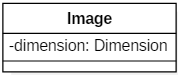
\includegraphics[width=0.5\linewidth]{images/view/classes/Image}
\end{figure} 
\subsubsection{Declaration}{
\begin{lstlisting}[frame=none]
public class Image
 extends java.lang.Object\end{lstlisting}
\subsubsection{Constructor summary}{
\begin{verse}
\hyperlink{Grid.Image()}{{\bf Image()}} Default constructor\\
\end{verse}
}
\subsubsection{Constructors}{
\vskip -2em
\begin{itemize}
\item{ 
\index{Image()}
\hypertarget{Grid.Image()}{{\bf  Image}\\}
\begin{lstlisting}[frame=none]
public Image()\end{lstlisting} %end signature
\begin{itemize}
\item{
{\bf  Description}

Default constructor
}
\end{itemize}
}%end item
\end{itemize}
}
}
\subsection{\label{Grid.ImageTile}Class ImageTile}{
\hypertarget{Grid.ImageTile}{}\vskip .1in 
A Tile whose graphical representation consists of an image.\vskip .1in 
\begin{figure}[!hbp]
	\centering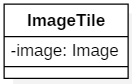
\includegraphics[width=0.5\linewidth]{images/view/classes/ImageTile}
\end{figure} 
\subsubsection{Declaration}{
\begin{lstlisting}[frame=none]
public class ImageTile
 extends Grid.Tile\end{lstlisting}
\subsubsection{Constructor summary}{
\begin{verse}
\hyperlink{Grid.ImageTile()}{{\bf ImageTile()}} Default constructor\\
\end{verse}
}
\subsubsection{Constructors}{
\vskip -2em
\begin{itemize}
\item{ 
\index{ImageTile()}
\hypertarget{Grid.ImageTile()}{{\bf  ImageTile}\\}
\begin{lstlisting}[frame=none]
public ImageTile()\end{lstlisting} %end signature
\begin{itemize}
\item{
{\bf  Description}

Default constructor
}
\end{itemize}
}%end item
\end{itemize}
}
\subsubsection{Members inherited from class Tile }{
\texttt{Grid.Tile} {\small 
\refdefined{Grid.Tile}}
{\small 

\vskip -2em
\begin{itemize}
\item{\vskip -1.5ex 
\texttt{protected {\bf  color}}%end signature
}%end item
\item{\vskip -1.5ex 
\texttt{public void {\bf  display}(\texttt{java.util.AbstractMap} {\bf  map})
}%end signature
}%end item
\item{\vskip -1.5ex 
\texttt{protected {\bf  opacity}}%end signature
}%end item
\item{\vskip -1.5ex 
\texttt{protected {\bf  position}}%end signature
}%end item
\item{\vskip -1.5ex 
\texttt{public void {\bf  setColor}(\texttt{Color} {\bf  color})
}%end signature
}%end item
\item{\vskip -1.5ex 
\texttt{public void {\bf  setOpacity}(\texttt{float} {\bf  opacity})
}%end signature
}%end item
\item{\vskip -1.5ex 
\texttt{public void {\bf  setPosition}(\texttt{Point} {\bf  position})
}%end signature
}%end item
\end{itemize}
}
}
\subsection{\label{Grid.ShapeTile}Class ShapeTile}{
\hypertarget{Grid.ShapeTile}{}\vskip .1in 
A Tile whose graphical representation consists of a shape, specified by an array of vertices.\vskip .1in
\begin{figure}[!hbp]
	\centering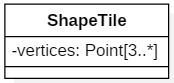
\includegraphics[width=0.5\linewidth]{images/view/classes/ShapeTile}
\end{figure} 
\subsubsection{Declaration}{
\begin{lstlisting}[frame=none]
public class ShapeTile
 extends Grid.Tile\end{lstlisting}
\subsubsection{Constructor summary}{
\begin{verse}
\hyperlink{Grid.ShapeTile()}{{\bf ShapeTile()}} Default constructor\\
\end{verse}
}
\subsubsection{Constructors}{
\vskip -2em
\begin{itemize}
\item{ 
\index{ShapeTile()}
\hypertarget{Grid.ShapeTile()}{{\bf  ShapeTile}\\}
\begin{lstlisting}[frame=none]
public ShapeTile()\end{lstlisting} %end signature
\begin{itemize}
\item{
{\bf  Description}

Default constructor
}
\end{itemize}
}%end item
\end{itemize}
}
\subsubsection{Members inherited from class Tile }{
\texttt{Grid.Tile} {\small 
\refdefined{Grid.Tile}}
{\small 

\vskip -2em
\begin{itemize}
\item{\vskip -1.5ex 
\texttt{protected {\bf  color}}%end signature
}%end item
\item{\vskip -1.5ex 
\texttt{public void {\bf  display}(\texttt{java.util.AbstractMap} {\bf  map})
}%end signature
}%end item
\item{\vskip -1.5ex 
\texttt{protected {\bf  opacity}}%end signature
}%end item
\item{\vskip -1.5ex 
\texttt{protected {\bf  position}}%end signature
}%end item
\item{\vskip -1.5ex 
\texttt{public void {\bf  setColor}(\texttt{Color} {\bf  color})
}%end signature
}%end item
\item{\vskip -1.5ex 
\texttt{public void {\bf  setOpacity}(\texttt{float} {\bf  opacity})
}%end signature
}%end item
\item{\vskip -1.5ex 
\texttt{public void {\bf  setPosition}(\texttt{Point} {\bf  position})
}%end signature
}%end item
\end{itemize}
}
}
\subsection{\label{Grid.Tile}Class Tile}{
\hypertarget{Grid.Tile}{}\vskip .1in 
A graphical structure that can be displayed on an AbstractMap.\vskip .1in 
\begin{figure}[!hbp]
	\centering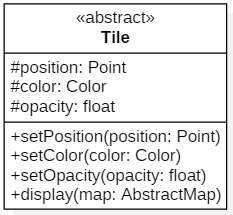
\includegraphics[width=0.5\linewidth]{images/view/classes/Tile}
\end{figure} 
\subsubsection{Declaration}{
\begin{lstlisting}[frame=none]
public class Tile
 extends java.lang.Object\end{lstlisting}
\subsubsection{All known subclasses}{ShapeTile\small{\refdefined{Grid.ShapeTile}}, ImageTile\small{\refdefined{Grid.ImageTile}}}
\subsubsection{Field summary}{
\begin{verse}
\hyperlink{Grid.Tile.color}{{\bf color}} \\
\hyperlink{Grid.Tile.opacity}{{\bf opacity}} \\
\hyperlink{Grid.Tile.position}{{\bf position}} \\
\end{verse}
}
\subsubsection{Constructor summary}{
\begin{verse}
\hyperlink{Grid.Tile()}{{\bf Tile()}} Default constructor\\
\end{verse}
}
\subsubsection{Method summary}{
\begin{verse}
\hyperlink{Grid.Tile.display(java.util.AbstractMap)}{{\bf display(AbstractMap)}} Display this tile on the submitted map.\\
\hyperlink{Grid.Tile.setColor(Color)}{{\bf setColor(Color)}} Set the color of this Tile.\\
\hyperlink{Grid.Tile.setOpacity(float)}{{\bf setOpacity(float)}} Set the opacity of this Tile.\\
\hyperlink{Grid.Tile.setPosition(Point)}{{\bf setPosition(Point)}} Set the position of this Tile.\\
\end{verse}
}
\subsubsection{Fields}{
\begin{itemize}
\item{
\index{position}
\label{Grid.Tile.position}\hypertarget{Grid.Tile.position}{\texttt{protected Point\ {\bf  position}}
}
}
\item{
\index{color}
\label{Grid.Tile.color}\hypertarget{Grid.Tile.color}{\texttt{protected Color\ {\bf  color}}
}
}
\item{
\index{opacity}
\label{Grid.Tile.opacity}\hypertarget{Grid.Tile.opacity}{\texttt{protected float\ {\bf  opacity}}
}
}
\end{itemize}
}
\subsubsection{Constructors}{
\vskip -2em
\begin{itemize}
\item{ 
\index{Tile()}
\hypertarget{Grid.Tile()}{{\bf  Tile}\\}
\begin{lstlisting}[frame=none]
public Tile()\end{lstlisting} %end signature
\begin{itemize}
\item{
{\bf  Description}

Default constructor
}
\end{itemize}
}%end item
\end{itemize}
}
\subsubsection{Methods}{
\vskip -2em
\begin{itemize}
\item{ 
\index{display(AbstractMap)}
\hypertarget{Grid.Tile.display(java.util.AbstractMap)}{{\bf  display}\\}
\begin{lstlisting}[frame=none]
public void display(java.util.AbstractMap map)\end{lstlisting} %end signature
\begin{itemize}
\item{
{\bf  Description}

Display this tile on the submitted map.
}
\item{
{\bf  Parameters}
  \begin{itemize}
   \item{
\texttt{map} -- }
  \end{itemize}
}%end item
\end{itemize}
}%end item
\item{ 
\index{setColor(Color)}
\hypertarget{Grid.Tile.setColor(Color)}{{\bf  setColor}\\}
\begin{lstlisting}[frame=none]
public void setColor(Color color)\end{lstlisting} %end signature
\begin{itemize}
\item{
{\bf  Description}

Set the color of this Tile.
}
\item{
{\bf  Parameters}
  \begin{itemize}
   \item{
\texttt{color} -- }
  \end{itemize}
}%end item
\end{itemize}
}%end item
\item{ 
\index{setOpacity(float)}
\hypertarget{Grid.Tile.setOpacity(float)}{{\bf  setOpacity}\\}
\begin{lstlisting}[frame=none]
public void setOpacity(float opacity)\end{lstlisting} %end signature
\begin{itemize}
\item{
{\bf  Description}

Set the opacity of this Tile.
}
\item{
{\bf  Parameters}
  \begin{itemize}
   \item{
\texttt{opacity} -- }
  \end{itemize}
}%end item
\end{itemize}
}%end item
\item{ 
\index{setPosition(Point)}
\hypertarget{Grid.Tile.setPosition(Point)}{{\bf  setPosition}\\}
\begin{lstlisting}[frame=none]
public void setPosition(Point position)\end{lstlisting} %end signature
\begin{itemize}
\item{
{\bf  Description}

Set the position of this Tile.
}
\item{
{\bf  Parameters}
  \begin{itemize}
   \item{
\texttt{position} -- }
  \end{itemize}
}%end item
\end{itemize}
}%end item
\end{itemize}
}
}
}
\section{Package View}{
\label{View}\hypertarget{View}{}
\hskip -.05in
\hbox to \hsize{\textit{ Package Contents\hfil Page}}
\vskip .13in
\hbox{{\bf  Classes}}
\entityintro{AbstractView}{View.AbstractView}{Encapsulates all ViewComponents created by the AbstractViewFactory into a single object.}
\entityintro{AbstractViewFactory}{View.AbstractViewFactory}{A factory for the creation of a View.}
\entityintro{View}{View.View}{An implementation of AbstractView.}
\entityintro{ViewComponent}{View.ViewComponent}{A view component which the View is made up of.}
\entityintro{ViewFactory}{View.ViewFactory}{An Implementation of AbstractViewFactory.}
\entityintro{ViewManager}{View.ViewManager}{Initializes and runs the AbstractView.}
\vskip .1in
\vskip .1in
\subsection{\label{View.AbstractView}Class AbstractView}{
\hypertarget{View.AbstractView}{}\vskip .1in 
Encapsulates all ViewComponents created by the AbstractViewFactory into a single object.\vskip .1in 
\begin{figure}[!hbp]
	\centering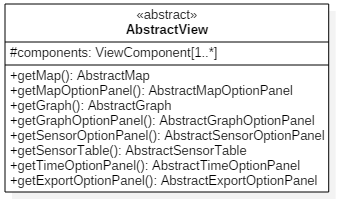
\includegraphics[width=0.5\linewidth]{images/view/classes/AbstractView}
\end{figure} 
\subsubsection{Declaration}{
\begin{lstlisting}[frame=none]
public class AbstractView
 extends java.lang.Object\end{lstlisting}
\subsubsection{All known subclasses}{View\small{\refdefined{View.View}}}
\subsubsection{Constructor summary}{
\begin{verse}
\hyperlink{View.AbstractView()}{{\bf AbstractView()}} Default constructor\\
\end{verse}
}
\subsubsection{Method summary}{
\begin{verse}
\hyperlink{View.AbstractView.getExportOptionPanel()}{{\bf getExportOptionPanel()}} Get the AbstractExportOptionPanel.\\
\hyperlink{View.AbstractView.getGraph()}{{\bf getGraph()}} Get the AbstractGraph.\\
\hyperlink{View.AbstractView.getGraphOptionPanel()}{{\bf getGraphOptionPanel()}} Get the AbstractGraphOptionPanel.\\
\hyperlink{View.AbstractView.getMap()}{{\bf getMap()}} Get the AbstractMap.\\
\hyperlink{View.AbstractView.getMapOptionPanel()}{{\bf getMapOptionPanel()}} Get the AbstractMapOptionPanel.\\
\hyperlink{View.AbstractView.getSensorOptionPanel()}{{\bf getSensorOptionPanel()}} Get the AbstractSensorOptionPanel.\\
\hyperlink{View.AbstractView.getSensorTable()}{{\bf getSensorTable()}} Get the AbstractSensorTable.\\
\hyperlink{View.AbstractView.getTimeOptionPanel()}{{\bf getTimeOptionPanel()}} Get the AbstractTimeOptionPanel.\\
\end{verse}
}
\subsubsection{Constructors}{
\vskip -2em
\begin{itemize}
\item{ 
\index{AbstractView()}
\hypertarget{View.AbstractView()}{{\bf  AbstractView}\\}
\begin{lstlisting}[frame=none]
public AbstractView()\end{lstlisting} %end signature
\begin{itemize}
\item{
{\bf  Description}

Default constructor
}
\end{itemize}
}%end item
\end{itemize}
}
\subsubsection{Methods}{
\vskip -2em
\begin{itemize}
\item{ 
\index{getExportOptionPanel()}
\hypertarget{View.AbstractView.getExportOptionPanel()}{{\bf  getExportOptionPanel}\\}
\begin{lstlisting}[frame=none]
public AbstractExportOptionPanel getExportOptionPanel()\end{lstlisting} %end signature
\begin{itemize}
\item{
{\bf  Description}

Get the AbstractExportOptionPanel.
}
\item{{\bf  Returns} -- 
the AbstractExportOptionPanel. 
}%end item
\end{itemize}
}%end item
\item{ 
\index{getGraph()}
\hypertarget{View.AbstractView.getGraph()}{{\bf  getGraph}\\}
\begin{lstlisting}[frame=none]
public AbstractGraph getGraph()\end{lstlisting} %end signature
\begin{itemize}
\item{
{\bf  Description}

Get the AbstractGraph.
}
\item{{\bf  Returns} -- 
the AbstractGraph. 
}%end item
\end{itemize}
}%end item
\item{ 
\index{getGraphOptionPanel()}
\hypertarget{View.AbstractView.getGraphOptionPanel()}{{\bf  getGraphOptionPanel}\\}
\begin{lstlisting}[frame=none]
public AbstractGraphOptionPanel getGraphOptionPanel()\end{lstlisting} %end signature
\begin{itemize}
\item{
{\bf  Description}

Get the AbstractGraphOptionPanel.
}
\item{{\bf  Returns} -- 
the AbstractGraphOptionPanel. 
}%end item
\end{itemize}
}%end item
\item{ 
\index{getMap()}
\hypertarget{View.AbstractView.getMap()}{{\bf  getMap}\\}
\begin{lstlisting}[frame=none]
public java.util.AbstractMap getMap()\end{lstlisting} %end signature
\begin{itemize}
\item{
{\bf  Description}

Get the AbstractMap.
}
\item{{\bf  Returns} -- 
the AbstractMap. 
}%end item
\end{itemize}
}%end item
\item{ 
\index{getMapOptionPanel()}
\hypertarget{View.AbstractView.getMapOptionPanel()}{{\bf  getMapOptionPanel}\\}
\begin{lstlisting}[frame=none]
public AbstractMapOptionPanel getMapOptionPanel()\end{lstlisting} %end signature
\begin{itemize}
\item{
{\bf  Description}

Get the AbstractMapOptionPanel.
}
\item{{\bf  Returns} -- 
the AbstractMapOptionPanel. 
}%end item
\end{itemize}
}%end item
\item{ 
\index{getSensorOptionPanel()}
\hypertarget{View.AbstractView.getSensorOptionPanel()}{{\bf  getSensorOptionPanel}\\}
\begin{lstlisting}[frame=none]
public AbstractSensorOptionPanel getSensorOptionPanel()\end{lstlisting} %end signature
\begin{itemize}
\item{
{\bf  Description}

Get the AbstractSensorOptionPanel.
}
\item{{\bf  Returns} -- 
the AbstractSensorOptionPanel. 
}%end item
\end{itemize}
}%end item
\item{ 
\index{getSensorTable()}
\hypertarget{View.AbstractView.getSensorTable()}{{\bf  getSensorTable}\\}
\begin{lstlisting}[frame=none]
public AbstractSensorTable getSensorTable()\end{lstlisting} %end signature
\begin{itemize}
\item{
{\bf  Description}

Get the AbstractSensorTable.
}
\item{{\bf  Returns} -- 
the AbstractSensorTable. 
}%end item
\end{itemize}
}%end item
\item{ 
\index{getTimeOptionPanel()}
\hypertarget{View.AbstractView.getTimeOptionPanel()}{{\bf  getTimeOptionPanel}\\}
\begin{lstlisting}[frame=none]
public AbstractTimeOptionPanel getTimeOptionPanel()\end{lstlisting} %end signature
\begin{itemize}
\item{
{\bf  Description}

Get the AbstractTimeOptionPanel.
}
\item{{\bf  Returns} -- 
the AbstractTimeOptionPanel. 
}%end item
\end{itemize}
}%end item
\end{itemize}
}
}
\subsection{\label{View.AbstractViewFactory}Class AbstractViewFactory}{
\hypertarget{View.AbstractViewFactory}{}\vskip .1in 
A factory for the creation of a View.\vskip .1in 
\begin{figure}[!hbp]
	\centering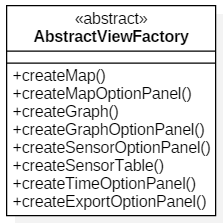
\includegraphics[width=0.5\linewidth]{images/view/classes/AbstractViewFactory}
\end{figure} 
\subsubsection{Declaration}{
\begin{lstlisting}[frame=none]
public class AbstractViewFactory
 extends java.lang.Object\end{lstlisting}
\subsubsection{All known subclasses}{ViewFactory\small{\refdefined{View.ViewFactory}}}
\subsubsection{Constructor summary}{
\begin{verse}
\hyperlink{View.AbstractViewFactory()}{{\bf AbstractViewFactory()}} Default constructor\\
\end{verse}
}
\subsubsection{Method summary}{
\begin{verse}
\hyperlink{View.AbstractViewFactory.createExportOptionPanel()}{{\bf createExportOptionPanel()}} Create an AbstractExportOptionPanel.\\
\hyperlink{View.AbstractViewFactory.createGraph()}{{\bf createGraph()}} Create an AbstractGraph.\\
\hyperlink{View.AbstractViewFactory.createGraphOptionPanel()}{{\bf createGraphOptionPanel()}} Create an AbstractGraphOptionPanel.\\
\hyperlink{View.AbstractViewFactory.createMap()}{{\bf createMap()}} Create an AbstractMap.\\
\hyperlink{View.AbstractViewFactory.createMapOptionPanel()}{{\bf createMapOptionPanel()}} Create an AbstractMapOptionPanel.\\
\hyperlink{View.AbstractViewFactory.createSensorOptionPanel()}{{\bf createSensorOptionPanel()}} Create an AbstractSensorOptionPanel.\\
\hyperlink{View.AbstractViewFactory.createSensorTable()}{{\bf createSensorTable()}} Create an AbstractSensorTable.\\
\hyperlink{View.AbstractViewFactory.createTimeOptionPanel()}{{\bf createTimeOptionPanel()}} Create an AbstractTimeOptionPanel.\\
\end{verse}
}
\subsubsection{Constructors}{
\vskip -2em
\begin{itemize}
\item{ 
\index{AbstractViewFactory()}
\hypertarget{View.AbstractViewFactory()}{{\bf  AbstractViewFactory}\\}
\begin{lstlisting}[frame=none]
public AbstractViewFactory()\end{lstlisting} %end signature
\begin{itemize}
\item{
{\bf  Description}

Default constructor
}
\end{itemize}
}%end item
\end{itemize}
}
\subsubsection{Methods}{
\vskip -2em
\begin{itemize}
\item{ 
\index{createExportOptionPanel()}
\hypertarget{View.AbstractViewFactory.createExportOptionPanel()}{{\bf  createExportOptionPanel}\\}
\begin{lstlisting}[frame=none]
public void createExportOptionPanel()\end{lstlisting} %end signature
\begin{itemize}
\item{
{\bf  Description}

Create an AbstractExportOptionPanel.
}
\end{itemize}
}%end item
\item{ 
\index{createGraph()}
\hypertarget{View.AbstractViewFactory.createGraph()}{{\bf  createGraph}\\}
\begin{lstlisting}[frame=none]
public void createGraph()\end{lstlisting} %end signature
\begin{itemize}
\item{
{\bf  Description}

Create an AbstractGraph.
}
\end{itemize}
}%end item
\item{ 
\index{createGraphOptionPanel()}
\hypertarget{View.AbstractViewFactory.createGraphOptionPanel()}{{\bf  createGraphOptionPanel}\\}
\begin{lstlisting}[frame=none]
public void createGraphOptionPanel()\end{lstlisting} %end signature
\begin{itemize}
\item{
{\bf  Description}

Create an AbstractGraphOptionPanel.
}
\end{itemize}
}%end item
\item{ 
\index{createMap()}
\hypertarget{View.AbstractViewFactory.createMap()}{{\bf  createMap}\\}
\begin{lstlisting}[frame=none]
public void createMap()\end{lstlisting} %end signature
\begin{itemize}
\item{
{\bf  Description}

Create an AbstractMap.
}
\end{itemize}
}%end item
\item{ 
\index{createMapOptionPanel()}
\hypertarget{View.AbstractViewFactory.createMapOptionPanel()}{{\bf  createMapOptionPanel}\\}
\begin{lstlisting}[frame=none]
public void createMapOptionPanel()\end{lstlisting} %end signature
\begin{itemize}
\item{
{\bf  Description}

Create an AbstractMapOptionPanel.
}
\end{itemize}
}%end item
\item{ 
\index{createSensorOptionPanel()}
\hypertarget{View.AbstractViewFactory.createSensorOptionPanel()}{{\bf  createSensorOptionPanel}\\}
\begin{lstlisting}[frame=none]
public void createSensorOptionPanel()\end{lstlisting} %end signature
\begin{itemize}
\item{
{\bf  Description}

Create an AbstractSensorOptionPanel.
}
\end{itemize}
}%end item
\item{ 
\index{createSensorTable()}
\hypertarget{View.AbstractViewFactory.createSensorTable()}{{\bf  createSensorTable}\\}
\begin{lstlisting}[frame=none]
public void createSensorTable()\end{lstlisting} %end signature
\begin{itemize}
\item{
{\bf  Description}

Create an AbstractSensorTable.
}
\end{itemize}
}%end item
\item{ 
\index{createTimeOptionPanel()}
\hypertarget{View.AbstractViewFactory.createTimeOptionPanel()}{{\bf  createTimeOptionPanel}\\}
\begin{lstlisting}[frame=none]
public void createTimeOptionPanel()\end{lstlisting} %end signature
\begin{itemize}
\item{
{\bf  Description}

Create an AbstractTimeOptionPanel.
}
\end{itemize}
}%end item
\end{itemize}
}
}
\subsection{\label{View.View}Class View}{
\hypertarget{View.View}{}\vskip .1in 
An implementation of AbstractView.\vskip .1in 
\begin{figure}[!hbp]
	\centering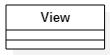
\includegraphics[width=0.5\linewidth]{images/view/classes/View}
\end{figure} 
\subsubsection{Declaration}{
\begin{lstlisting}[frame=none]
public class View
 extends View.AbstractView\end{lstlisting}
\subsubsection{Constructor summary}{
\begin{verse}
\hyperlink{View.View()}{{\bf View()}} Default constructor\\
\end{verse}
}
\subsubsection{Constructors}{
\vskip -2em
\begin{itemize}
\item{ 
\index{View()}
\hypertarget{View.View()}{{\bf  View}\\}
\begin{lstlisting}[frame=none]
public View()\end{lstlisting} %end signature
\begin{itemize}
\item{
{\bf  Description}

Default constructor
}
\end{itemize}
}%end item
\end{itemize}
}
\subsubsection{Members inherited from class AbstractView }{
\texttt{View.AbstractView} {\small 
\refdefined{View.AbstractView}}
{\small 

\vskip -2em
\begin{itemize}
\item{\vskip -1.5ex 
\texttt{public AbstractExportOptionPanel {\bf  getExportOptionPanel}()
}%end signature
}%end item
\item{\vskip -1.5ex 
\texttt{public AbstractGraph {\bf  getGraph}()
}%end signature
}%end item
\item{\vskip -1.5ex 
\texttt{public AbstractGraphOptionPanel {\bf  getGraphOptionPanel}()
}%end signature
}%end item
\item{\vskip -1.5ex 
\texttt{public AbstractMap {\bf  getMap}()
}%end signature
}%end item
\item{\vskip -1.5ex 
\texttt{public AbstractMapOptionPanel {\bf  getMapOptionPanel}()
}%end signature
}%end item
\item{\vskip -1.5ex 
\texttt{public AbstractSensorOptionPanel {\bf  getSensorOptionPanel}()
}%end signature
}%end item
\item{\vskip -1.5ex 
\texttt{public AbstractSensorTable {\bf  getSensorTable}()
}%end signature
}%end item
\item{\vskip -1.5ex 
\texttt{public AbstractTimeOptionPanel {\bf  getTimeOptionPanel}()
}%end signature
}%end item
\end{itemize}
}
}
\subsection{\label{View.ViewComponent}Class ViewComponent}{
\hypertarget{View.ViewComponent}{}\vskip .1in 
A view component which the View is made up of.\vskip .1in 
\begin{figure}[!hbp]
	\centering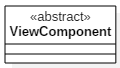
\includegraphics[width=0.5\linewidth]{images/view/classes/ViewComponent}
\end{figure} 
\subsubsection{Declaration}{
\begin{lstlisting}[frame=none]
public class ViewComponent
 extends java.lang.Object\end{lstlisting}
\subsubsection{Constructor summary}{
\begin{verse}
\hyperlink{View.ViewComponent()}{{\bf ViewComponent()}} Default constructor\\
\end{verse}
}
\subsubsection{Constructors}{
\vskip -2em
\begin{itemize}
\item{ 
\index{ViewComponent()}
\hypertarget{View.ViewComponent()}{{\bf  ViewComponent}\\}
\begin{lstlisting}[frame=none]
public ViewComponent()\end{lstlisting} %end signature
\begin{itemize}
\item{
{\bf  Description}

Default constructor
}
\end{itemize}
}%end item
\end{itemize}
}
}
\subsection{\label{View.ViewFactory}Class ViewFactory}{
\hypertarget{View.ViewFactory}{}\vskip .1in 
An Implementation of AbstractViewFactory.\vskip .1in 
\begin{figure}[!hbp]
	\centering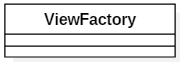
\includegraphics[width=0.5\linewidth]{images/view/classes/ViewFactory}
\end{figure} 
\subsubsection{Declaration}{
\begin{lstlisting}[frame=none]
public class ViewFactory
 extends View.AbstractViewFactory\end{lstlisting}
\subsubsection{Constructor summary}{
\begin{verse}
\hyperlink{View.ViewFactory()}{{\bf ViewFactory()}} Default constructor\\
\end{verse}
}
\subsubsection{Constructors}{
\vskip -2em
\begin{itemize}
\item{ 
\index{ViewFactory()}
\hypertarget{View.ViewFactory()}{{\bf  ViewFactory}\\}
\begin{lstlisting}[frame=none]
public ViewFactory()\end{lstlisting} %end signature
\begin{itemize}
\item{
{\bf  Description}

Default constructor
}
\end{itemize}
}%end item
\end{itemize}
}
\subsubsection{Members inherited from class AbstractViewFactory }{
\texttt{View.AbstractViewFactory} {\small 
\refdefined{View.AbstractViewFactory}}
{\small 

\vskip -2em
\begin{itemize}
\item{\vskip -1.5ex 
\texttt{public void {\bf  createExportOptionPanel}()
}%end signature
}%end item
\item{\vskip -1.5ex 
\texttt{public void {\bf  createGraph}()
}%end signature
}%end item
\item{\vskip -1.5ex 
\texttt{public void {\bf  createGraphOptionPanel}()
}%end signature
}%end item
\item{\vskip -1.5ex 
\texttt{public void {\bf  createMap}()
}%end signature
}%end item
\item{\vskip -1.5ex 
\texttt{public void {\bf  createMapOptionPanel}()
}%end signature
}%end item
\item{\vskip -1.5ex 
\texttt{public void {\bf  createSensorOptionPanel}()
}%end signature
}%end item
\item{\vskip -1.5ex 
\texttt{public void {\bf  createSensorTable}()
}%end signature
}%end item
\item{\vskip -1.5ex 
\texttt{public void {\bf  createTimeOptionPanel}()
}%end signature
}%end item
\end{itemize}
}
}
\subsection{\label{View.ViewManager}Class ViewManager}{
\hypertarget{View.ViewManager}{}\vskip .1in 
Initializes and runs the AbstractView.\vskip .1in 
\begin{figure}[!hbp]
	\centering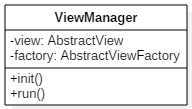
\includegraphics[width=0.5\linewidth]{images/view/classes/ViewManager}
\end{figure} 
\subsubsection{Declaration}{
\begin{lstlisting}[frame=none]
public class ViewManager
 extends java.lang.Object\end{lstlisting}
\subsubsection{Constructor summary}{
\begin{verse}
\hyperlink{View.ViewManager()}{{\bf ViewManager()}} Default constructor\\
\end{verse}
}
\subsubsection{Method summary}{
\begin{verse}
\hyperlink{View.ViewManager.init()}{{\bf init()}} Initializes the ViewManager by creating the View and its ViewComponents.\\
\hyperlink{View.ViewManager.run()}{{\bf run()}} Run the View by looping the refresh method located in the AbstractTimeOptionPanel in your AbstractView.\\
\end{verse}
}
\subsubsection{Constructors}{
\vskip -2em
\begin{itemize}
\item{ 
\index{ViewManager()}
\hypertarget{View.ViewManager()}{{\bf  ViewManager}\\}
\begin{lstlisting}[frame=none]
public ViewManager()\end{lstlisting} %end signature
\begin{itemize}
\item{
{\bf  Description}

Default constructor
}
\end{itemize}
}%end item
\end{itemize}
}
\subsubsection{Methods}{
\vskip -2em
\begin{itemize}
\item{ 
\index{init()}
\hypertarget{View.ViewManager.init()}{{\bf  init}\\}
\begin{lstlisting}[frame=none]
public void init()\end{lstlisting} %end signature
\begin{itemize}
\item{
{\bf  Description}

Initializes the ViewManager by creating the View and its ViewComponents.
}
\end{itemize}
}%end item
\item{ 
\index{run()}
\hypertarget{View.ViewManager.run()}{{\bf  run}\\}
\begin{lstlisting}[frame=none]
public void run()\end{lstlisting} %end signature
\begin{itemize}
\item{
{\bf  Description}

Run the View by looping the refresh method located in the AbstractTimeOptionPanel in your AbstractView.
}
\end{itemize}
}%end item
\end{itemize}
}
}
}
\section{Package View.ExportOption}{
\label{View.ExportOption}\hypertarget{View.ExportOption}{}
\hskip -.05in
\hbox to \hsize{\textit{ Package Contents\hfil Page}}
\vskip .13in
\hbox{{\bf  Classes}}
\entityintro{AbstractExportOptionPanel}{View.ExportOption.AbstractExportOptionPanel}{A panel for handling user input, that deals with exporting datasets.}
\entityintro{ExportOptionPanel}{View.ExportOption.ExportOptionPanel}{An implementation of AbstractExportOptionPanel.}
\vskip .1in
\vskip .1in
\subsection{\label{View.ExportOption.AbstractExportOptionPanel}Class AbstractExportOptionPanel}{
\hypertarget{View.ExportOption.AbstractExportOptionPanel}{}\vskip .1in 
A panel for handling user input, that deals with exporting datasets. The user can select Clusters by their ClusterIDs, Sensors by their SensorIDs, a time frame, sensor types and a file format.\vskip .1in 
\begin{figure}[!hbp]
	\centering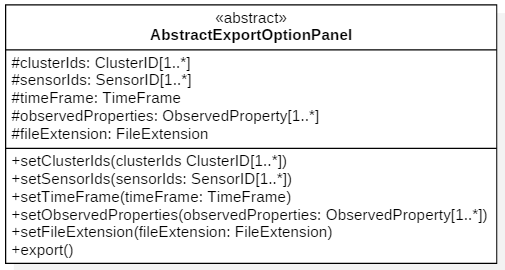
\includegraphics[width=0.5\linewidth]{images/view/classes/AbstractExportOptionPanel}
\end{figure} 
\subsubsection{Declaration}{
\begin{lstlisting}[frame=none]
public class AbstractExportOptionPanel
 extends ViewComponent\end{lstlisting}
\subsubsection{All known subclasses}{ExportOptionPanel\small{\refdefined{View.ExportOption.ExportOptionPanel}}}
\subsubsection{Field summary}{
\begin{verse}
\hyperlink{View.ExportOption.AbstractExportOptionPanel.clusterIds}{{\bf clusterIds}} \\
\hyperlink{View.ExportOption.AbstractExportOptionPanel.fileExtension}{{\bf fileExtension}} \\
\hyperlink{View.ExportOption.AbstractExportOptionPanel.observedProperties}{{\bf observedProperties}} \\
\hyperlink{View.ExportOption.AbstractExportOptionPanel.sensorIds}{{\bf sensorIds}} \\
\hyperlink{View.ExportOption.AbstractExportOptionPanel.timeFrame}{{\bf timeFrame}} \\
\end{verse}
}
\subsubsection{Constructor summary}{
\begin{verse}
\hyperlink{View.ExportOption.AbstractExportOptionPanel()}{{\bf AbstractExportOptionPanel()}} Default constructor\\
\end{verse}
}
\subsubsection{Method summary}{
\begin{verse}
\hyperlink{View.ExportOption.AbstractExportOptionPanel.export()}{{\bf export()}} Request an export with the given parameters.\\
\hyperlink{View.ExportOption.AbstractExportOptionPanel.mapUpdate()}{{\bf mapUpdate()}} \\
\hyperlink{View.ExportOption.AbstractExportOptionPanel.sensorOptionUpdate()}{{\bf sensorOptionUpdate()}} Update the observer with the current SensorOptionPanel state.\\
\hyperlink{View.ExportOption.AbstractExportOptionPanel.setClusterIds(java.util.Set)}{{\bf setClusterIds(Set)}} Set the ClusterIDs.\\
\hyperlink{View.ExportOption.AbstractExportOptionPanel.setFileExtension(FileExtension)}{{\bf setFileExtension(FileExtension)}} Set the ExportFormat.\\
\hyperlink{View.ExportOption.AbstractExportOptionPanel.setObservedProperties(java.util.Set)}{{\bf setObservedProperties(Set)}} Set the SensorTypes.\\
\hyperlink{View.ExportOption.AbstractExportOptionPanel.setSensorIds(java.util.Set)}{{\bf setSensorIds(Set)}} Set the SensorIDs.\\
\hyperlink{View.ExportOption.AbstractExportOptionPanel.setTimeFrame(TimeFrame)}{{\bf setTimeFrame(TimeFrame)}} Set the TimeFrame.\\
\hyperlink{View.ExportOption.AbstractExportOptionPanel.timeOptionUpdate()}{{\bf timeOptionUpdate()}} Update the observer with the current TimeOptionPanel state.\\
\end{verse}
}
\subsubsection{Fields}{
\begin{itemize}
\item{
\index{clusterIds}
\label{View.ExportOption.AbstractExportOptionPanel.clusterIds}\hypertarget{View.ExportOption.AbstractExportOptionPanel.clusterIds}{\texttt{protected java.util.Set\ {\bf  clusterIds}}
}
}
\item{
\index{sensorIds}
\label{View.ExportOption.AbstractExportOptionPanel.sensorIds}\hypertarget{View.ExportOption.AbstractExportOptionPanel.sensorIds}{\texttt{protected java.util.Set\ {\bf  sensorIds}}
}
}
\item{
\index{timeFrame}
\label{View.ExportOption.AbstractExportOptionPanel.timeFrame}\hypertarget{View.ExportOption.AbstractExportOptionPanel.timeFrame}{\texttt{protected TimeFrame\ {\bf  timeFrame}}
}
}
\item{
\index{observedProperties}
\label{View.ExportOption.AbstractExportOptionPanel.observedProperties}\hypertarget{View.ExportOption.AbstractExportOptionPanel.observedProperties}{\texttt{protected java.util.Set\ {\bf  observedProperties}}
}
}
\item{
\index{fileExtension}
\label{View.ExportOption.AbstractExportOptionPanel.fileExtension}\hypertarget{View.ExportOption.AbstractExportOptionPanel.fileExtension}{\texttt{protected FileExtension\ {\bf  fileExtension}}
}
}
\end{itemize}
}
\subsubsection{Constructors}{
\vskip -2em
\begin{itemize}
\item{ 
\index{AbstractExportOptionPanel()}
\hypertarget{View.ExportOption.AbstractExportOptionPanel()}{{\bf  AbstractExportOptionPanel}\\}
\begin{lstlisting}[frame=none]
public AbstractExportOptionPanel()\end{lstlisting} %end signature
\begin{itemize}
\item{
{\bf  Description}

Default constructor
}
\end{itemize}
}%end item
\end{itemize}
}
\subsubsection{Methods}{
\vskip -2em
\begin{itemize}
\item{ 
\index{export()}
\hypertarget{View.ExportOption.AbstractExportOptionPanel.export()}{{\bf  export}\\}
\begin{lstlisting}[frame=none]
public void export()\end{lstlisting} %end signature
\begin{itemize}
\item{
{\bf  Description}

Request an export with the given parameters.
}
\end{itemize}
}%end item
\item{ 
\index{mapUpdate()}
\hypertarget{View.ExportOption.AbstractExportOptionPanel.mapUpdate()}{{\bf  mapUpdate}\\}
\begin{lstlisting}[frame=none]
public void mapUpdate()\end{lstlisting} %end signature
}%end item
\item{ 
\index{sensorOptionUpdate()}
\hypertarget{View.ExportOption.AbstractExportOptionPanel.sensorOptionUpdate()}{{\bf  sensorOptionUpdate}\\}
\begin{lstlisting}[frame=none]
public void sensorOptionUpdate()\end{lstlisting} %end signature
\begin{itemize}
\item{
{\bf  Description}

Update the observer with the current SensorOptionPanel state.
}
\end{itemize}
}%end item
\item{ 
\index{setClusterIds(Set)}
\hypertarget{View.ExportOption.AbstractExportOptionPanel.setClusterIds(java.util.Set)}{{\bf  setClusterIds}\\}
\begin{lstlisting}[frame=none]
public void setClusterIds(java.util.Set clusterIds)\end{lstlisting} %end signature
\begin{itemize}
\item{
{\bf  Description}

Set the ClusterIDs.
}
\item{
{\bf  Parameters}
  \begin{itemize}
   \item{
\texttt{clusterIds} -- }
  \end{itemize}
}%end item
\end{itemize}
}%end item
\item{ 
\index{setFileExtension(FileExtension)}
\hypertarget{View.ExportOption.AbstractExportOptionPanel.setFileExtension(FileExtension)}{{\bf  setFileExtension}\\}
\begin{lstlisting}[frame=none]
public void setFileExtension(FileExtension fileExtension)\end{lstlisting} %end signature
\begin{itemize}
\item{
{\bf  Description}

Set the ExportFormat.
}
\item{
{\bf  Parameters}
  \begin{itemize}
   \item{
\texttt{fileExtension} -- }
  \end{itemize}
}%end item
\end{itemize}
}%end item
\item{ 
\index{setObservedProperties(Set)}
\hypertarget{View.ExportOption.AbstractExportOptionPanel.setObservedProperties(java.util.Set)}{{\bf  setObservedProperties}\\}
\begin{lstlisting}[frame=none]
public void setObservedProperties(java.util.Set observedProperties)\end{lstlisting} %end signature
\begin{itemize}
\item{
{\bf  Description}

Set the SensorTypes.
}
\item{
{\bf  Parameters}
  \begin{itemize}
   \item{
\texttt{observedProperties} -- }
  \end{itemize}
}%end item
\end{itemize}
}%end item
\item{ 
\index{setSensorIds(Set)}
\hypertarget{View.ExportOption.AbstractExportOptionPanel.setSensorIds(java.util.Set)}{{\bf  setSensorIds}\\}
\begin{lstlisting}[frame=none]
public void setSensorIds(java.util.Set sensorIds)\end{lstlisting} %end signature
\begin{itemize}
\item{
{\bf  Description}

Set the SensorIDs.
}
\item{
{\bf  Parameters}
  \begin{itemize}
   \item{
\texttt{sensorIds} -- }
  \end{itemize}
}%end item
\end{itemize}
}%end item
\item{ 
\index{setTimeFrame(TimeFrame)}
\hypertarget{View.ExportOption.AbstractExportOptionPanel.setTimeFrame(TimeFrame)}{{\bf  setTimeFrame}\\}
\begin{lstlisting}[frame=none]
public void setTimeFrame(TimeFrame timeFrame)\end{lstlisting} %end signature
\begin{itemize}
\item{
{\bf  Description}

Set the TimeFrame.
}
\item{
{\bf  Parameters}
  \begin{itemize}
   \item{
\texttt{timeFrame} -- }
  \end{itemize}
}%end item
\end{itemize}
}%end item
\item{ 
\index{timeOptionUpdate()}
\hypertarget{View.ExportOption.AbstractExportOptionPanel.timeOptionUpdate()}{{\bf  timeOptionUpdate}\\}
\begin{lstlisting}[frame=none]
public void timeOptionUpdate()\end{lstlisting} %end signature
\begin{itemize}
\item{
{\bf  Description}

Update the observer with the current TimeOptionPanel state.
}
\end{itemize}
}%end item
\end{itemize}
}
}
\subsection{\label{View.ExportOption.ExportOptionPanel}Class ExportOptionPanel}{
\hypertarget{View.ExportOption.ExportOptionPanel}{}\vskip .1in 
An implementation of AbstractExportOptionPanel.\vskip .1in 
\begin{figure}[!hbp]
	\centering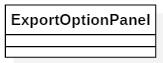
\includegraphics[width=0.5\linewidth]{images/view/classes/ExportOptionPanel}
\end{figure} 
\subsubsection{Declaration}{
\begin{lstlisting}[frame=none]
public class ExportOptionPanel
 extends View.ExportOption.AbstractExportOptionPanel\end{lstlisting}
\subsubsection{Constructor summary}{
\begin{verse}
\hyperlink{View.ExportOption.ExportOptionPanel()}{{\bf ExportOptionPanel()}} Default constructor\\
\end{verse}
}
\subsubsection{Constructors}{
\vskip -2em
\begin{itemize}
\item{ 
\index{ExportOptionPanel()}
\hypertarget{View.ExportOption.ExportOptionPanel()}{{\bf  ExportOptionPanel}\\}
\begin{lstlisting}[frame=none]
public ExportOptionPanel()\end{lstlisting} %end signature
\begin{itemize}
\item{
{\bf  Description}

Default constructor
}
\end{itemize}
}%end item
\end{itemize}
}
\subsubsection{Members inherited from class AbstractExportOptionPanel }{
\texttt{View.ExportOption.AbstractExportOptionPanel} {\small 
\refdefined{View.ExportOption.AbstractExportOptionPanel}}
{\small 

\vskip -2em
\begin{itemize}
\item{\vskip -1.5ex 
\texttt{protected {\bf  clusterIds}}%end signature
}%end item
\item{\vskip -1.5ex 
\texttt{public void {\bf  export}()
}%end signature
}%end item
\item{\vskip -1.5ex 
\texttt{protected {\bf  fileExtension}}%end signature
}%end item
\item{\vskip -1.5ex 
\texttt{public void {\bf  mapUpdate}()
}%end signature
}%end item
\item{\vskip -1.5ex 
\texttt{protected {\bf  observedProperties}}%end signature
}%end item
\item{\vskip -1.5ex 
\texttt{protected {\bf  sensorIds}}%end signature
}%end item
\item{\vskip -1.5ex 
\texttt{public void {\bf  sensorOptionUpdate}()
}%end signature
}%end item
\item{\vskip -1.5ex 
\texttt{public void {\bf  setClusterIds}(\texttt{java.util.Set} {\bf  clusterIds})
}%end signature
}%end item
\item{\vskip -1.5ex 
\texttt{public void {\bf  setFileExtension}(\texttt{FileExtension} {\bf  fileExtension})
}%end signature
}%end item
\item{\vskip -1.5ex 
\texttt{public void {\bf  setObservedProperties}(\texttt{java.util.Set} {\bf  observedProperties})
}%end signature
}%end item
\item{\vskip -1.5ex 
\texttt{public void {\bf  setSensorIds}(\texttt{java.util.Set} {\bf  sensorIds})
}%end signature
}%end item
\item{\vskip -1.5ex 
\texttt{public void {\bf  setTimeFrame}(\texttt{TimeFrame} {\bf  timeFrame})
}%end signature
}%end item
\item{\vskip -1.5ex 
\texttt{protected {\bf  timeFrame}}%end signature
}%end item
\item{\vskip -1.5ex 
\texttt{public void {\bf  timeOptionUpdate}()
}%end signature
}%end item
\end{itemize}
}
}
}
\section{Package View.Graph}{
\label{View.Graph}\hypertarget{View.Graph}{}
\hskip -.05in
\hbox to \hsize{\textit{ Package Contents\hfil Page}}
\vskip .13in
\hbox{{\bf  Interfaces}}
\entityintro{GraphOptionPanelObserver}{View.Graph.GraphOptionPanelObserver}{An observer that is meant to observe changes in the GraphOptionPanel.}
\vskip .13in
\hbox{{\bf  Classes}}
\entityintro{AbstractGraph}{View.Graph.AbstractGraph}{A graph that visualizes the data in its dataset.}
\entityintro{AbstractGraphOptionPanel}{View.Graph.AbstractGraphOptionPanel}{A panel for handling user input, that deals with which time segment of the graphs dataset is being displayed, how that is done and notifying all observers about changes in its state.}
\entityintro{GraphDisplayType}{View.Graph.GraphDisplayType}{The display type of a graph.}
\entityintro{GraphiteGraph}{View.Graph.GraphiteGraph}{An AbstractGraph that uses the Graphite API.}
\entityintro{GraphOptionPanel}{View.Graph.GraphOptionPanel}{An implementation of AbstractGraphOptionPanel.}
\vskip .1in
\vskip .1in
\subsection{\label{View.Graph.GraphOptionPanelObserver}Interface GraphOptionPanelObserver}{
\hypertarget{View.Graph.GraphOptionPanelObserver}{}\vskip .1in 
An observer that is meant to observe changes in the GraphOptionPanel.\vskip .1in 
\begin{figure}[!hbp]
	\centering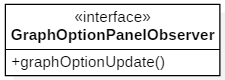
\includegraphics[width=0.5\linewidth]{images/view/classes/GraphOptionPanelObserver}
\end{figure} 
\subsubsection{Declaration}{
\begin{lstlisting}[frame=none]
public interface GraphOptionPanelObserver
\end{lstlisting}
\subsubsection{All known subinterfaces}{GraphiteGraph\small{\refdefined{View.Graph.GraphiteGraph}}, AbstractGraph\small{\refdefined{View.Graph.AbstractGraph}}}
\subsubsection{All classes known to implement interface}{AbstractGraph\small{\refdefined{View.Graph.AbstractGraph}}}
\subsubsection{Method summary}{
\begin{verse}
\hyperlink{View.Graph.GraphOptionPanelObserver.graphOptionUpdate()}{{\bf graphOptionUpdate()}} Update the observer with the current GraphOptionPanel state.\\
\end{verse}
}
\subsubsection{Methods}{
\vskip -2em
\begin{itemize}
\item{ 
\index{graphOptionUpdate()}
\hypertarget{View.Graph.GraphOptionPanelObserver.graphOptionUpdate()}{{\bf  graphOptionUpdate}\\}
\begin{lstlisting}[frame=none]
void graphOptionUpdate()\end{lstlisting} %end signature
\begin{itemize}
\item{
{\bf  Description}

Update the observer with the current GraphOptionPanel state.
}
\end{itemize}
}%end item
\end{itemize}
}
}
\subsection{\label{View.Graph.AbstractGraph}Class AbstractGraph}{
\hypertarget{View.Graph.AbstractGraph}{}\vskip .1in 
A graph that visualizes the data in its dataset.\vskip .1in 
\begin{figure}[!hbp]
	\centering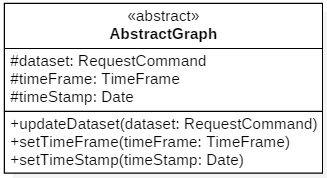
\includegraphics[width=0.5\linewidth]{images/view/classes/AbstractGraph}
\end{figure} 
\subsubsection{Declaration}{
\begin{lstlisting}[frame=none]
public class AbstractGraph
 extends ViewComponent implements GraphOptionPanelObserver\end{lstlisting}
\subsubsection{All known subclasses}{GraphiteGraph\small{\refdefined{View.Graph.GraphiteGraph}}}
\subsubsection{Field summary}{
\begin{verse}
\hyperlink{View.Graph.AbstractGraph.dataset}{{\bf dataset}} \\
\hyperlink{View.Graph.AbstractGraph.timeFrame}{{\bf timeFrame}} \\
\hyperlink{View.Graph.AbstractGraph.timeStamp}{{\bf timeStamp}} \\
\end{verse}
}
\subsubsection{Constructor summary}{
\begin{verse}
\hyperlink{View.Graph.AbstractGraph()}{{\bf AbstractGraph()}} Default constructor\\
\end{verse}
}
\subsubsection{Method summary}{
\begin{verse}
\hyperlink{View.Graph.AbstractGraph.graphOptionUpdate()}{{\bf graphOptionUpdate()}} Update the observer with the current GraphOptionPanel state.\\
\hyperlink{View.Graph.AbstractGraph.mapUpdate()}{{\bf mapUpdate()}} \\
\hyperlink{View.Graph.AbstractGraph.sensorOptionUpdate()}{{\bf sensorOptionUpdate()}} Update the observer with the current SensorOptionPanel state.\\
\hyperlink{View.Graph.AbstractGraph.setTimeFrame(TimeFrame)}{{\bf setTimeFrame(TimeFrame)}} Set the starting and end time point of the displayed dataset segment.\\
\hyperlink{View.Graph.AbstractGraph.setTimeStamp(java.util.Date)}{{\bf setTimeStamp(Date)}} Set a time stamp.\\
\hyperlink{View.Graph.AbstractGraph.timeOptionUpdate()}{{\bf timeOptionUpdate()}} Update the observer with the current TimeOptionPanel state.\\
\hyperlink{View.Graph.AbstractGraph.updateDataset(RequestCommand)}{{\bf updateDataset(RequestCommand)}} Update the dataset of this AbstractGraph by giving it a new RequestCommand.\\
\end{verse}
}
\subsubsection{Fields}{
\begin{itemize}
\item{
\index{dataset}
\label{View.Graph.AbstractGraph.dataset}\hypertarget{View.Graph.AbstractGraph.dataset}{\texttt{protected RequestCommand\ {\bf  dataset}}
}
}
\item{
\index{timeFrame}
\label{View.Graph.AbstractGraph.timeFrame}\hypertarget{View.Graph.AbstractGraph.timeFrame}{\texttt{protected TimeFrame\ {\bf  timeFrame}}
}
}
\item{
\index{timeStamp}
\label{View.Graph.AbstractGraph.timeStamp}\hypertarget{View.Graph.AbstractGraph.timeStamp}{\texttt{protected java.util.Date\ {\bf  timeStamp}}
}
}
\end{itemize}
}
\subsubsection{Constructors}{
\vskip -2em
\begin{itemize}
\item{ 
\index{AbstractGraph()}
\hypertarget{View.Graph.AbstractGraph()}{{\bf  AbstractGraph}\\}
\begin{lstlisting}[frame=none]
public AbstractGraph()\end{lstlisting} %end signature
\begin{itemize}
\item{
{\bf  Description}

Default constructor
}
\end{itemize}
}%end item
\end{itemize}
}
\subsubsection{Methods}{
\vskip -2em
\begin{itemize}
\item{ 
\index{graphOptionUpdate()}
\hypertarget{View.Graph.AbstractGraph.graphOptionUpdate()}{{\bf  graphOptionUpdate}\\}
\begin{lstlisting}[frame=none]
public void graphOptionUpdate()\end{lstlisting} %end signature
\begin{itemize}
\item{
{\bf  Description}

Update the observer with the current GraphOptionPanel state.
}
\end{itemize}
}%end item
\item{ 
\index{mapUpdate()}
\hypertarget{View.Graph.AbstractGraph.mapUpdate()}{{\bf  mapUpdate}\\}
\begin{lstlisting}[frame=none]
public void mapUpdate()\end{lstlisting} %end signature
}%end item
\item{ 
\index{sensorOptionUpdate()}
\hypertarget{View.Graph.AbstractGraph.sensorOptionUpdate()}{{\bf  sensorOptionUpdate}\\}
\begin{lstlisting}[frame=none]
public void sensorOptionUpdate()\end{lstlisting} %end signature
\begin{itemize}
\item{
{\bf  Description}

Update the observer with the current SensorOptionPanel state.
}
\end{itemize}
}%end item
\item{ 
\index{setTimeFrame(TimeFrame)}
\hypertarget{View.Graph.AbstractGraph.setTimeFrame(TimeFrame)}{{\bf  setTimeFrame}\\}
\begin{lstlisting}[frame=none]
public void setTimeFrame(TimeFrame timeFrame)\end{lstlisting} %end signature
\begin{itemize}
\item{
{\bf  Description}

Set the starting and end time point of the displayed dataset segment.
}
\item{
{\bf  Parameters}
  \begin{itemize}
   \item{
\texttt{timeFrame} -- }
  \end{itemize}
}%end item
\end{itemize}
}%end item
\item{ 
\index{setTimeStamp(Date)}
\hypertarget{View.Graph.AbstractGraph.setTimeStamp(java.util.Date)}{{\bf  setTimeStamp}\\}
\begin{lstlisting}[frame=none]
public void setTimeStamp(java.util.Date timeStamp)\end{lstlisting} %end signature
\begin{itemize}
\item{
{\bf  Description}

Set a time stamp.
}
\item{
{\bf  Parameters}
  \begin{itemize}
   \item{
\texttt{timeStamp} -- }
  \end{itemize}
}%end item
\end{itemize}
}%end item
\item{ 
\index{timeOptionUpdate()}
\hypertarget{View.Graph.AbstractGraph.timeOptionUpdate()}{{\bf  timeOptionUpdate}\\}
\begin{lstlisting}[frame=none]
public void timeOptionUpdate()\end{lstlisting} %end signature
\begin{itemize}
\item{
{\bf  Description}

Update the observer with the current TimeOptionPanel state.
}
\end{itemize}
}%end item
\item{ 
\index{updateDataset(RequestCommand)}
\hypertarget{View.Graph.AbstractGraph.updateDataset(RequestCommand)}{{\bf  updateDataset}\\}
\begin{lstlisting}[frame=none]
public void updateDataset(RequestCommand dataset)\end{lstlisting} %end signature
\begin{itemize}
\item{
{\bf  Description}

Update the dataset of this AbstractGraph by giving it a new RequestCommand.
}
\item{
{\bf  Parameters}
  \begin{itemize}
   \item{
\texttt{dataset} -- }
  \end{itemize}
}%end item
\end{itemize}
}%end item
\end{itemize}
}
}
\subsection{\label{View.Graph.AbstractGraphOptionPanel}Class AbstractGraphOptionPanel}{
\hypertarget{View.Graph.AbstractGraphOptionPanel}{}\vskip .1in 
A panel for handling user input, that deals with which time segment of the graphs dataset is being displayed, how that is done and notifying all observers about changes in its state.\vskip .1in 
\begin{figure}[!hbp]
	\centering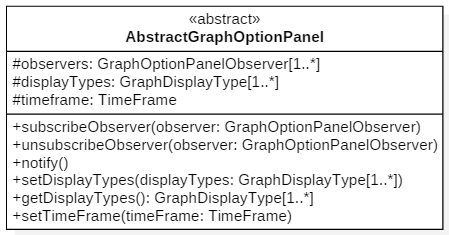
\includegraphics[width=0.5\linewidth]{images/view/classes/AbstractGraphOptionPanel}
\end{figure} 
\subsubsection{Declaration}{
\begin{lstlisting}[frame=none]
public class AbstractGraphOptionPanel
 extends ViewComponent\end{lstlisting}
\subsubsection{All known subclasses}{GraphOptionPanel\small{\refdefined{View.Graph.GraphOptionPanel}}}
\subsubsection{Field summary}{
\begin{verse}
\hyperlink{View.Graph.AbstractGraphOptionPanel.timeframe}{{\bf timeframe}} \\
\end{verse}
}
\subsubsection{Constructor summary}{
\begin{verse}
\hyperlink{View.Graph.AbstractGraphOptionPanel()}{{\bf AbstractGraphOptionPanel()}} Default constructor\\
\end{verse}
}
\subsubsection{Method summary}{
\begin{verse}
\hyperlink{View.Graph.AbstractGraphOptionPanel.getDisplayTypes()}{{\bf getDisplayTypes()}} Get the GraphDisplayTypes.\\
\hyperlink{View.Graph.AbstractGraphOptionPanel.notify()}{{\bf notify()}} Notify all subscribed GraphOptionPanelObservers about a change in this AbstractGraphOptionPanel.\\
\hyperlink{View.Graph.AbstractGraphOptionPanel.setDisplayTypes(java.util.Set)}{{\bf setDisplayTypes(Set)}} Set the GraphDisplayTypes.\\
\hyperlink{View.Graph.AbstractGraphOptionPanel.setTimeFrame(TimeFrame)}{{\bf setTimeFrame(TimeFrame)}} Set the starting and end time point of the displayed dataset segment..\\
\hyperlink{View.Graph.AbstractGraphOptionPanel.subscribeObserver(View.Graph.GraphOptionPanelObserver)}{{\bf subscribeObserver(GraphOptionPanelObserver)}} Subscribe a GraphOptionPanelObserver to this AbstractGraphOptionPanel.\\
\hyperlink{View.Graph.AbstractGraphOptionPanel.unsubscribeObserver(View.Graph.GraphOptionPanelObserver)}{{\bf unsubscribeObserver(GraphOptionPanelObserver)}} Unsubscribe a GraphOptionPanelObserver from this AbstractGraphOptionPanel.\\
\end{verse}
}
\subsubsection{Fields}{
\begin{itemize}
\item{
\index{timeframe}
\label{View.Graph.AbstractGraphOptionPanel.timeframe}\hypertarget{View.Graph.AbstractGraphOptionPanel.timeframe}{\texttt{protected TimeFrame\ {\bf  timeframe}}
}
}
\end{itemize}
}
\subsubsection{Constructors}{
\vskip -2em
\begin{itemize}
\item{ 
\index{AbstractGraphOptionPanel()}
\hypertarget{View.Graph.AbstractGraphOptionPanel()}{{\bf  AbstractGraphOptionPanel}\\}
\begin{lstlisting}[frame=none]
public AbstractGraphOptionPanel()\end{lstlisting} %end signature
\begin{itemize}
\item{
{\bf  Description}

Default constructor
}
\end{itemize}
}%end item
\end{itemize}
}
\subsubsection{Methods}{
\vskip -2em
\begin{itemize}
\item{ 
\index{getDisplayTypes()}
\hypertarget{View.Graph.AbstractGraphOptionPanel.getDisplayTypes()}{{\bf  getDisplayTypes}\\}
\begin{lstlisting}[frame=none]
public java.util.Set getDisplayTypes()\end{lstlisting} %end signature
\begin{itemize}
\item{
{\bf  Description}

Get the GraphDisplayTypes.
}
\item{{\bf  Returns} -- 
the GraphDisplayTypes. 
}%end item
\end{itemize}
}%end item
\item{ 
\index{notify()}
\hypertarget{View.Graph.AbstractGraphOptionPanel.notify()}{{\bf  notify}\\}
\begin{lstlisting}[frame=none]
public void notify()\end{lstlisting} %end signature
\begin{itemize}
\item{
{\bf  Description}

Notify all subscribed GraphOptionPanelObservers about a change in this AbstractGraphOptionPanel.
}
\end{itemize}
}%end item
\item{ 
\index{setDisplayTypes(Set)}
\hypertarget{View.Graph.AbstractGraphOptionPanel.setDisplayTypes(java.util.Set)}{{\bf  setDisplayTypes}\\}
\begin{lstlisting}[frame=none]
public void setDisplayTypes(java.util.Set displayTypes)\end{lstlisting} %end signature
\begin{itemize}
\item{
{\bf  Description}

Set the GraphDisplayTypes.
}
\item{
{\bf  Parameters}
  \begin{itemize}
   \item{
\texttt{displayTypes} -- }
  \end{itemize}
}%end item
\end{itemize}
}%end item
\item{ 
\index{setTimeFrame(TimeFrame)}
\hypertarget{View.Graph.AbstractGraphOptionPanel.setTimeFrame(TimeFrame)}{{\bf  setTimeFrame}\\}
\begin{lstlisting}[frame=none]
public void setTimeFrame(TimeFrame timeFrame)\end{lstlisting} %end signature
\begin{itemize}
\item{
{\bf  Description}

Set the starting and end time point of the displayed dataset segment..
}
\item{
{\bf  Parameters}
  \begin{itemize}
   \item{
\texttt{timeFrame} -- }
  \end{itemize}
}%end item
\end{itemize}
}%end item
\item{ 
\index{subscribeObserver(GraphOptionPanelObserver)}
\hypertarget{View.Graph.AbstractGraphOptionPanel.subscribeObserver(View.Graph.GraphOptionPanelObserver)}{{\bf  subscribeObserver}\\}
\begin{lstlisting}[frame=none]
public void subscribeObserver(GraphOptionPanelObserver observer)\end{lstlisting} %end signature
\begin{itemize}
\item{
{\bf  Description}

Subscribe a GraphOptionPanelObserver to this AbstractGraphOptionPanel.
}
\item{
{\bf  Parameters}
  \begin{itemize}
   \item{
\texttt{observer} -- }
  \end{itemize}
}%end item
\end{itemize}
}%end item
\item{ 
\index{unsubscribeObserver(GraphOptionPanelObserver)}
\hypertarget{View.Graph.AbstractGraphOptionPanel.unsubscribeObserver(View.Graph.GraphOptionPanelObserver)}{{\bf  unsubscribeObserver}\\}
\begin{lstlisting}[frame=none]
public void unsubscribeObserver(GraphOptionPanelObserver observer)\end{lstlisting} %end signature
\begin{itemize}
\item{
{\bf  Description}

Unsubscribe a GraphOptionPanelObserver from this AbstractGraphOptionPanel.
}
\item{
{\bf  Parameters}
  \begin{itemize}
   \item{
\texttt{observer} -- }
  \end{itemize}
}%end item
\end{itemize}
}%end item
\end{itemize}
}
}
\subsection{\label{View.Graph.GraphDisplayType}Class GraphDisplayType}{
\hypertarget{View.Graph.GraphDisplayType}{}\vskip .1in 
The display type of a graph.\vskip .1in 
\begin{figure}[!hbp]
	\centering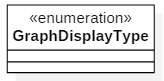
\includegraphics[width=0.5\linewidth]{images/view/classes/GraphDisplayType}
\end{figure} 
\subsubsection{Declaration}{
\begin{lstlisting}[frame=none]
public class GraphDisplayType
 extends java.lang.Object\end{lstlisting}
\subsubsection{Constructor summary}{
\begin{verse}
\hyperlink{View.Graph.GraphDisplayType()}{{\bf GraphDisplayType()}} Default constructor\\
\end{verse}
}
\subsubsection{Constructors}{
\vskip -2em
\begin{itemize}
\item{ 
\index{GraphDisplayType()}
\hypertarget{View.Graph.GraphDisplayType()}{{\bf  GraphDisplayType}\\}
\begin{lstlisting}[frame=none]
public GraphDisplayType()\end{lstlisting} %end signature
\begin{itemize}
\item{
{\bf  Description}

Default constructor
}
\end{itemize}
}%end item
\end{itemize}
}
}
\subsection{\label{View.Graph.GraphiteGraph}Class GraphiteGraph}{
\hypertarget{View.Graph.GraphiteGraph}{}\vskip .1in 
An AbstractGraph that uses the Graphite API.\vskip .1in 
\begin{figure}[!hbp]
	\centering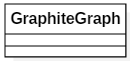
\includegraphics[width=0.5\linewidth]{images/view/classes/GraphiteGraph}
\end{figure} 
\subsubsection{Declaration}{
\begin{lstlisting}[frame=none]
public class GraphiteGraph
 extends View.Graph.AbstractGraph\end{lstlisting}
\subsubsection{Constructor summary}{
\begin{verse}
\hyperlink{View.Graph.GraphiteGraph()}{{\bf GraphiteGraph()}} Default constructor\\
\end{verse}
}
\subsubsection{Constructors}{
\vskip -2em
\begin{itemize}
\item{ 
\index{GraphiteGraph()}
\hypertarget{View.Graph.GraphiteGraph()}{{\bf  GraphiteGraph}\\}
\begin{lstlisting}[frame=none]
public GraphiteGraph()\end{lstlisting} %end signature
\begin{itemize}
\item{
{\bf  Description}

Default constructor
}
\end{itemize}
}%end item
\end{itemize}
}
\subsubsection{Members inherited from class AbstractGraph }{
\texttt{View.Graph.AbstractGraph} {\small 
\refdefined{View.Graph.AbstractGraph}}
{\small 

\vskip -2em
\begin{itemize}
\item{\vskip -1.5ex 
\texttt{protected {\bf  dataset}}%end signature
}%end item
\item{\vskip -1.5ex 
\texttt{public void {\bf  graphOptionUpdate}()
}%end signature
}%end item
\item{\vskip -1.5ex 
\texttt{public void {\bf  mapUpdate}()
}%end signature
}%end item
\item{\vskip -1.5ex 
\texttt{public void {\bf  sensorOptionUpdate}()
}%end signature
}%end item
\item{\vskip -1.5ex 
\texttt{public void {\bf  setTimeFrame}(\texttt{TimeFrame} {\bf  timeFrame})
}%end signature
}%end item
\item{\vskip -1.5ex 
\texttt{public void {\bf  setTimeStamp}(\texttt{java.util.Date} {\bf  timeStamp})
}%end signature
}%end item
\item{\vskip -1.5ex 
\texttt{protected {\bf  timeFrame}}%end signature
}%end item
\item{\vskip -1.5ex 
\texttt{public void {\bf  timeOptionUpdate}()
}%end signature
}%end item
\item{\vskip -1.5ex 
\texttt{protected {\bf  timeStamp}}%end signature
}%end item
\item{\vskip -1.5ex 
\texttt{public void {\bf  updateDataset}(\texttt{RequestCommand} {\bf  dataset})
}%end signature
}%end item
\end{itemize}
}
}
\subsection{\label{View.Graph.GraphOptionPanel}Class GraphOptionPanel}{
\hypertarget{View.Graph.GraphOptionPanel}{}\vskip .1in 
An implementation of AbstractGraphOptionPanel.\vskip .1in 
\begin{figure}[!hbp]
	\centering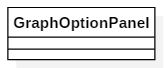
\includegraphics[width=0.5\linewidth]{images/view/classes/GraphOptionPanel}
\end{figure} 
\subsubsection{Declaration}{
\begin{lstlisting}[frame=none]
public class GraphOptionPanel
 extends View.Graph.AbstractGraphOptionPanel\end{lstlisting}
\subsubsection{Constructor summary}{
\begin{verse}
\hyperlink{View.Graph.GraphOptionPanel()}{{\bf GraphOptionPanel()}} Default constructor\\
\end{verse}
}
\subsubsection{Constructors}{
\vskip -2em
\begin{itemize}
\item{ 
\index{GraphOptionPanel()}
\hypertarget{View.Graph.GraphOptionPanel()}{{\bf  GraphOptionPanel}\\}
\begin{lstlisting}[frame=none]
public GraphOptionPanel()\end{lstlisting} %end signature
\begin{itemize}
\item{
{\bf  Description}

Default constructor
}
\end{itemize}
}%end item
\end{itemize}
}
\subsubsection{Members inherited from class AbstractGraphOptionPanel }{
\texttt{View.Graph.AbstractGraphOptionPanel} {\small 
\refdefined{View.Graph.AbstractGraphOptionPanel}}
{\small 

\vskip -2em
\begin{itemize}
\item{\vskip -1.5ex 
\texttt{public Set {\bf  getDisplayTypes}()
}%end signature
}%end item
\item{\vskip -1.5ex 
\texttt{public void {\bf  notify}()
}%end signature
}%end item
\item{\vskip -1.5ex 
\texttt{public void {\bf  setDisplayTypes}(\texttt{java.util.Set} {\bf  displayTypes})
}%end signature
}%end item
\item{\vskip -1.5ex 
\texttt{public void {\bf  setTimeFrame}(\texttt{TimeFrame} {\bf  timeFrame})
}%end signature
}%end item
\item{\vskip -1.5ex 
\texttt{public void {\bf  subscribeObserver}(\texttt{GraphOptionPanelObserver} {\bf  observer})
}%end signature
}%end item
\item{\vskip -1.5ex 
\texttt{protected {\bf  timeframe}}%end signature
}%end item
\item{\vskip -1.5ex 
\texttt{public void {\bf  unsubscribeObserver}(\texttt{GraphOptionPanelObserver} {\bf  observer})
}%end signature
}%end item
\end{itemize}
}
}
}
\section{Package View.Map}{
\label{View.Map}\hypertarget{View.Map}{}
\hskip -.05in
\hbox to \hsize{\textit{ Package Contents\hfil Page}}
\vskip .13in
\hbox{{\bf  Interfaces}}
\entityintro{MapObserver}{View.Map.MapObserver}{}
\entityintro{MapOptionPanelObserver}{View.Map.MapOptionPanelObserver}{An observer that is meant to observe changes in the MapOptionPanel.}
\vskip .13in
\hbox{{\bf  Classes}}
\entityintro{AbstractMap}{View.Map.AbstractMap}{A world map with displayable and hideable MapLayers, move and zoom function.}
\entityintro{AbstractMapOptionPanel}{View.Map.AbstractMapOptionPanel}{A panel for handling user input, that deals with setting a new TileType and notifying its observers about the change.}
\entityintro{LeafletMap}{View.Map.LeafletMap}{An AbstractMap that uses the Leaflet API.}
\entityintro{MapLayer}{View.Map.MapLayer}{A map layer that can be displayed on an AbstractMap.}
\entityintro{MapOptionPanel}{View.Map.MapOptionPanel}{An implementation of AbstractMapOptionPanel.}
\entityintro{TileType}{View.Map.TileType}{The type of a tile.}
\vskip .1in
\vskip .1in
\subsection{\label{View.Map.MapObserver}Interface MapObserver}{
\hypertarget{View.Map.MapObserver}{}\vskip .1in 
\begin{figure}[!hbp]
	\centering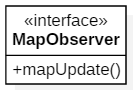
\includegraphics[width=0.5\linewidth]{images/view/classes/MapObserver}
\end{figure} 
\subsubsection{Declaration}{
\begin{lstlisting}[frame=none]
public interface MapObserver
\end{lstlisting}
\subsubsection{Method summary}{
\begin{verse}
\hyperlink{View.Map.MapObserver.mapUpdate()}{{\bf mapUpdate()}} \\
\end{verse}
}
\subsubsection{Methods}{
\vskip -2em
\begin{itemize}
\item{ 
\index{mapUpdate()}
\hypertarget{View.Map.MapObserver.mapUpdate()}{{\bf  mapUpdate}\\}
\begin{lstlisting}[frame=none]
void mapUpdate()\end{lstlisting} %end signature
}%end item
\end{itemize}
}
}
\subsection{\label{View.Map.MapOptionPanelObserver}Interface MapOptionPanelObserver}{
\hypertarget{View.Map.MapOptionPanelObserver}{}\vskip .1in 
An observer that is meant to observe changes in the MapOptionPanel.\vskip .1in 
\begin{figure}[!hbp]
	\centering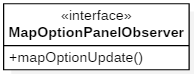
\includegraphics[width=0.5\linewidth]{images/view/classes/MapOptionPanelObserver}
\end{figure} 
\subsubsection{Declaration}{
\begin{lstlisting}[frame=none]
public interface MapOptionPanelObserver
\end{lstlisting}
\subsubsection{All known subinterfaces}{LeafletMap\small{\refdefined{View.Map.LeafletMap}}, AbstractMap\small{\refdefined{View.Map.AbstractMap}}}
\subsubsection{All classes known to implement interface}{AbstractMap\small{\refdefined{View.Map.AbstractMap}}}
\subsubsection{Method summary}{
\begin{verse}
\hyperlink{View.Map.MapOptionPanelObserver.mapOptionUpdate()}{{\bf mapOptionUpdate()}} Update the observer with the current MapOptionPanel state.\\
\end{verse}
}
\subsubsection{Methods}{
\vskip -2em
\begin{itemize}
\item{ 
\index{mapOptionUpdate()}
\hypertarget{View.Map.MapOptionPanelObserver.mapOptionUpdate()}{{\bf  mapOptionUpdate}\\}
\begin{lstlisting}[frame=none]
void mapOptionUpdate()\end{lstlisting} %end signature
\begin{itemize}
\item{
{\bf  Description}

Update the observer with the current MapOptionPanel state.
}
\end{itemize}
}%end item
\end{itemize}
}
}
\subsection{\label{View.Map.AbstractMap}Class AbstractMap}{
\hypertarget{View.Map.AbstractMap}{}\vskip .1in 
A world map with displayable and hideable MapLayers, move and zoom function. It notifies its observers about changes in its state.\vskip .1in 
\begin{figure}[!hbp]
	\centering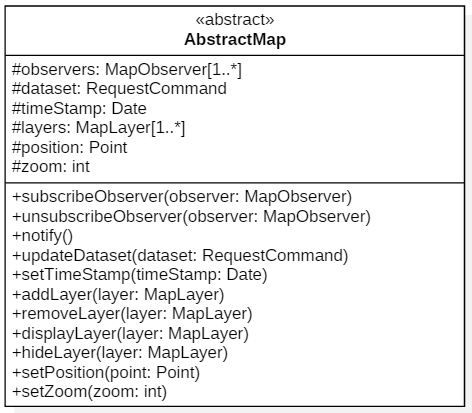
\includegraphics[width=0.5\linewidth]{images/view/classes/AbstractMap}
\end{figure} 
\subsubsection{Declaration}{
\begin{lstlisting}[frame=none]
public class AbstractMap
 extends ViewComponent implements MapOptionPanelObserver\end{lstlisting}
\subsubsection{All known subclasses}{LeafletMap\small{\refdefined{View.Map.LeafletMap}}}
\subsubsection{Field summary}{
\begin{verse}
\hyperlink{View.Map.AbstractMap.dataset}{{\bf dataset}} \\
\hyperlink{View.Map.AbstractMap.position}{{\bf position}} \\
\hyperlink{View.Map.AbstractMap.timeStamp}{{\bf timeStamp}} \\
\hyperlink{View.Map.AbstractMap.zoom}{{\bf zoom}} \\
\end{verse}
}
\subsubsection{Constructor summary}{
\begin{verse}
\hyperlink{View.Map.AbstractMap()}{{\bf AbstractMap()}} Default constructor\\
\end{verse}
}
\subsubsection{Method summary}{
\begin{verse}
\hyperlink{View.Map.AbstractMap.addLayer(View.Map.MapLayer)}{{\bf addLayer(MapLayer)}} Add a MapLayer.\\
\hyperlink{View.Map.AbstractMap.displayLayer(View.Map.MapLayer)}{{\bf displayLayer(MapLayer)}} Display a MapLayer.\\
\hyperlink{View.Map.AbstractMap.hideLayer(View.Map.MapLayer)}{{\bf hideLayer(MapLayer)}} Hide a MapLayer.\\
\hyperlink{View.Map.AbstractMap.mapOptionUpdate()}{{\bf mapOptionUpdate()}} Update the observer with the current MapOptionPanel state.\\
\hyperlink{View.Map.AbstractMap.notify()}{{\bf notify()}} Notify all subscribed MapObservers about a change in this AbstractMap.\\
\hyperlink{View.Map.AbstractMap.removeLayer(View.Map.MapLayer)}{{\bf removeLayer(MapLayer)}} Remove a MapLayer.\\
\hyperlink{View.Map.AbstractMap.sensorOptionUpdate()}{{\bf sensorOptionUpdate()}} Update the observer with the current SensorOptionPanel state.\\
\hyperlink{View.Map.AbstractMap.setPosition(Point)}{{\bf setPosition(Point)}} Set the center position of the AbstractMap.\\
\hyperlink{View.Map.AbstractMap.setTimeStamp(java.util.Date)}{{\bf setTimeStamp(Date)}} Set a time stamp and display the data from the dataset at the specified point in time.\\
\hyperlink{View.Map.AbstractMap.setZoom(int)}{{\bf setZoom(int)}} Set the zoom level of this AbstractMap.\\
\hyperlink{View.Map.AbstractMap.subscribeObserver(View.Map.MapObserver)}{{\bf subscribeObserver(MapObserver)}} Subscribe a MapObserver to this AbstractMap.\\
\hyperlink{View.Map.AbstractMap.timeOptionUpdate()}{{\bf timeOptionUpdate()}} Update the observer with the current TimeOptionPanel state.\\
\hyperlink{View.Map.AbstractMap.unsubscribeObserver(View.Map.MapObserver)}{{\bf unsubscribeObserver(MapObserver)}} Unsubscribe a MapObserver from this AbstractMap.\\
\hyperlink{View.Map.AbstractMap.updateDataset(RequestCommand)}{{\bf updateDataset(RequestCommand)}} Update the dataset of this AbstractMap by giving it a new RequestCommand.\\
\end{verse}
}
\subsubsection{Fields}{
\begin{itemize}
\item{
\index{dataset}
\label{View.Map.AbstractMap.dataset}\hypertarget{View.Map.AbstractMap.dataset}{\texttt{protected RequestCommand\ {\bf  dataset}}
}
}
\item{
\index{timeStamp}
\label{View.Map.AbstractMap.timeStamp}\hypertarget{View.Map.AbstractMap.timeStamp}{\texttt{protected java.util.Date\ {\bf  timeStamp}}
}
}
\item{
\index{position}
\label{View.Map.AbstractMap.position}\hypertarget{View.Map.AbstractMap.position}{\texttt{protected Point\ {\bf  position}}
}
}
\item{
\index{zoom}
\label{View.Map.AbstractMap.zoom}\hypertarget{View.Map.AbstractMap.zoom}{\texttt{protected int\ {\bf  zoom}}
}
}
\end{itemize}
}
\subsubsection{Constructors}{
\vskip -2em
\begin{itemize}
\item{ 
\index{AbstractMap()}
\hypertarget{View.Map.AbstractMap()}{{\bf  AbstractMap}\\}
\begin{lstlisting}[frame=none]
public AbstractMap()\end{lstlisting} %end signature
\begin{itemize}
\item{
{\bf  Description}

Default constructor
}
\end{itemize}
}%end item
\end{itemize}
}
\subsubsection{Methods}{
\vskip -2em
\begin{itemize}
\item{ 
\index{addLayer(MapLayer)}
\hypertarget{View.Map.AbstractMap.addLayer(View.Map.MapLayer)}{{\bf  addLayer}\\}
\begin{lstlisting}[frame=none]
public void addLayer(MapLayer layer)\end{lstlisting} %end signature
\begin{itemize}
\item{
{\bf  Description}

Add a MapLayer.
}
\item{
{\bf  Parameters}
  \begin{itemize}
   \item{
\texttt{layer} -- }
  \end{itemize}
}%end item
\end{itemize}
}%end item
\item{ 
\index{displayLayer(MapLayer)}
\hypertarget{View.Map.AbstractMap.displayLayer(View.Map.MapLayer)}{{\bf  displayLayer}\\}
\begin{lstlisting}[frame=none]
public void displayLayer(MapLayer layer)\end{lstlisting} %end signature
\begin{itemize}
\item{
{\bf  Description}

Display a MapLayer.
}
\item{
{\bf  Parameters}
  \begin{itemize}
   \item{
\texttt{layer} -- }
  \end{itemize}
}%end item
\end{itemize}
}%end item
\item{ 
\index{hideLayer(MapLayer)}
\hypertarget{View.Map.AbstractMap.hideLayer(View.Map.MapLayer)}{{\bf  hideLayer}\\}
\begin{lstlisting}[frame=none]
public void hideLayer(MapLayer layer)\end{lstlisting} %end signature
\begin{itemize}
\item{
{\bf  Description}

Hide a MapLayer.
}
\item{
{\bf  Parameters}
  \begin{itemize}
   \item{
\texttt{layer} -- }
  \end{itemize}
}%end item
\end{itemize}
}%end item
\item{ 
\index{mapOptionUpdate()}
\hypertarget{View.Map.AbstractMap.mapOptionUpdate()}{{\bf  mapOptionUpdate}\\}
\begin{lstlisting}[frame=none]
public void mapOptionUpdate()\end{lstlisting} %end signature
\begin{itemize}
\item{
{\bf  Description}

Update the observer with the current MapOptionPanel state.
}
\end{itemize}
}%end item
\item{ 
\index{notify()}
\hypertarget{View.Map.AbstractMap.notify()}{{\bf  notify}\\}
\begin{lstlisting}[frame=none]
public void notify()\end{lstlisting} %end signature
\begin{itemize}
\item{
{\bf  Description}

Notify all subscribed MapObservers about a change in this AbstractMap.
}
\end{itemize}
}%end item
\item{ 
\index{removeLayer(MapLayer)}
\hypertarget{View.Map.AbstractMap.removeLayer(View.Map.MapLayer)}{{\bf  removeLayer}\\}
\begin{lstlisting}[frame=none]
public void removeLayer(MapLayer layer)\end{lstlisting} %end signature
\begin{itemize}
\item{
{\bf  Description}

Remove a MapLayer.
}
\item{
{\bf  Parameters}
  \begin{itemize}
   \item{
\texttt{layer} -- }
  \end{itemize}
}%end item
\end{itemize}
}%end item
\item{ 
\index{sensorOptionUpdate()}
\hypertarget{View.Map.AbstractMap.sensorOptionUpdate()}{{\bf  sensorOptionUpdate}\\}
\begin{lstlisting}[frame=none]
public void sensorOptionUpdate()\end{lstlisting} %end signature
\begin{itemize}
\item{
{\bf  Description}

Update the observer with the current SensorOptionPanel state.
}
\end{itemize}
}%end item
\item{ 
\index{setPosition(Point)}
\hypertarget{View.Map.AbstractMap.setPosition(Point)}{{\bf  setPosition}\\}
\begin{lstlisting}[frame=none]
public void setPosition(Point point)\end{lstlisting} %end signature
\begin{itemize}
\item{
{\bf  Description}

Set the center position of the AbstractMap.
}
\item{
{\bf  Parameters}
  \begin{itemize}
   \item{
\texttt{point} -- }
  \end{itemize}
}%end item
\end{itemize}
}%end item
\item{ 
\index{setTimeStamp(Date)}
\hypertarget{View.Map.AbstractMap.setTimeStamp(java.util.Date)}{{\bf  setTimeStamp}\\}
\begin{lstlisting}[frame=none]
public void setTimeStamp(java.util.Date timeStamp)\end{lstlisting} %end signature
\begin{itemize}
\item{
{\bf  Description}

Set a time stamp and display the data from the dataset at the specified point in time.
}
\item{
{\bf  Parameters}
  \begin{itemize}
   \item{
\texttt{timeStamp} -- }
  \end{itemize}
}%end item
\end{itemize}
}%end item
\item{ 
\index{setZoom(int)}
\hypertarget{View.Map.AbstractMap.setZoom(int)}{{\bf  setZoom}\\}
\begin{lstlisting}[frame=none]
public void setZoom(int zoom)\end{lstlisting} %end signature
\begin{itemize}
\item{
{\bf  Description}

Set the zoom level of this AbstractMap.
}
\item{
{\bf  Parameters}
  \begin{itemize}
   \item{
\texttt{zoom} -- }
  \end{itemize}
}%end item
\end{itemize}
}%end item
\item{ 
\index{subscribeObserver(MapObserver)}
\hypertarget{View.Map.AbstractMap.subscribeObserver(View.Map.MapObserver)}{{\bf  subscribeObserver}\\}
\begin{lstlisting}[frame=none]
public void subscribeObserver(MapObserver observer)\end{lstlisting} %end signature
\begin{itemize}
\item{
{\bf  Description}

Subscribe a MapObserver to this AbstractMap.
}
\item{
{\bf  Parameters}
  \begin{itemize}
   \item{
\texttt{observer} -- }
  \end{itemize}
}%end item
\end{itemize}
}%end item
\item{ 
\index{timeOptionUpdate()}
\hypertarget{View.Map.AbstractMap.timeOptionUpdate()}{{\bf  timeOptionUpdate}\\}
\begin{lstlisting}[frame=none]
public void timeOptionUpdate()\end{lstlisting} %end signature
\begin{itemize}
\item{
{\bf  Description}

Update the observer with the current TimeOptionPanel state.
}
\end{itemize}
}%end item
\item{ 
\index{unsubscribeObserver(MapObserver)}
\hypertarget{View.Map.AbstractMap.unsubscribeObserver(View.Map.MapObserver)}{{\bf  unsubscribeObserver}\\}
\begin{lstlisting}[frame=none]
public void unsubscribeObserver(MapObserver observer)\end{lstlisting} %end signature
\begin{itemize}
\item{
{\bf  Description}

Unsubscribe a MapObserver from this AbstractMap.
}
\item{
{\bf  Parameters}
  \begin{itemize}
   \item{
\texttt{observer} -- }
  \end{itemize}
}%end item
\end{itemize}
}%end item
\item{ 
\index{updateDataset(RequestCommand)}
\hypertarget{View.Map.AbstractMap.updateDataset(RequestCommand)}{{\bf  updateDataset}\\}
\begin{lstlisting}[frame=none]
public void updateDataset(RequestCommand dataset)\end{lstlisting} %end signature
\begin{itemize}
\item{
{\bf  Description}

Update the dataset of this AbstractMap by giving it a new RequestCommand.
}
\item{
{\bf  Parameters}
  \begin{itemize}
   \item{
\texttt{dataset} -- }
  \end{itemize}
}%end item
\end{itemize}
}%end item
\end{itemize}
}
}
\subsection{\label{View.Map.AbstractMapOptionPanel}Class AbstractMapOptionPanel}{
\hypertarget{View.Map.AbstractMapOptionPanel}{}\vskip .1in 
A panel for handling user input, that deals with setting a new TileType and notifying its observers about the change.\vskip .1in 
\begin{figure}[!hbp]
	\centering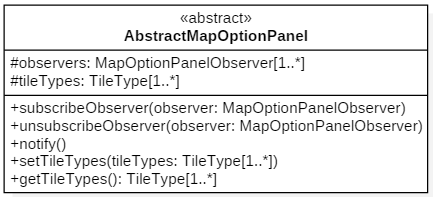
\includegraphics[width=0.5\linewidth]{images/view/classes/AbstractMapOptionPanel}
\end{figure} 
\subsubsection{Declaration}{
\begin{lstlisting}[frame=none]
public class AbstractMapOptionPanel
 extends ViewComponent\end{lstlisting}
\subsubsection{All known subclasses}{MapOptionPanel\small{\refdefined{View.Map.MapOptionPanel}}}
\subsubsection{Field summary}{
\begin{verse}
\hyperlink{View.Map.AbstractMapOptionPanel.observers}{{\bf observers}} \\
\end{verse}
}
\subsubsection{Constructor summary}{
\begin{verse}
\hyperlink{View.Map.AbstractMapOptionPanel()}{{\bf AbstractMapOptionPanel()}} Default constructor\\
\end{verse}
}
\subsubsection{Method summary}{
\begin{verse}
\hyperlink{View.Map.AbstractMapOptionPanel.getTileTypes()}{{\bf getTileTypes()}} Get the TileTypes.\\
\hyperlink{View.Map.AbstractMapOptionPanel.notify()}{{\bf notify()}} Notify all subscribed MapOptionPanelObservers about a change in this AbstractMapOptionPanel.\\
\hyperlink{View.Map.AbstractMapOptionPanel.setTileTypes(java.util.Set)}{{\bf setTileTypes(Set)}} Set the TileTypes.\\
\hyperlink{View.Map.AbstractMapOptionPanel.subscribeObserver(View.Map.MapOptionPanelObserver)}{{\bf subscribeObserver(MapOptionPanelObserver)}} Subscribe a MapOptionPanelObserver to this AbstractMapOptionPanel.\\
\hyperlink{View.Map.AbstractMapOptionPanel.unsubscribeObserver(View.Map.MapOptionPanelObserver)}{{\bf unsubscribeObserver(MapOptionPanelObserver)}} Unsubscribe a MapOptionPanelObserver from this AbstractMapOptionPanel.\\
\end{verse}
}
\subsubsection{Fields}{
\begin{itemize}
\item{
\index{observers}
\label{View.Map.AbstractMapOptionPanel.observers}\hypertarget{View.Map.AbstractMapOptionPanel.observers}{\texttt{protected java.util.Set\ {\bf  observers}}
}
}
\end{itemize}
}
\subsubsection{Constructors}{
\vskip -2em
\begin{itemize}
\item{ 
\index{AbstractMapOptionPanel()}
\hypertarget{View.Map.AbstractMapOptionPanel()}{{\bf  AbstractMapOptionPanel}\\}
\begin{lstlisting}[frame=none]
public AbstractMapOptionPanel()\end{lstlisting} %end signature
\begin{itemize}
\item{
{\bf  Description}

Default constructor
}
\end{itemize}
}%end item
\end{itemize}
}
\subsubsection{Methods}{
\vskip -2em
\begin{itemize}
\item{ 
\index{getTileTypes()}
\hypertarget{View.Map.AbstractMapOptionPanel.getTileTypes()}{{\bf  getTileTypes}\\}
\begin{lstlisting}[frame=none]
public java.util.Set getTileTypes()\end{lstlisting} %end signature
\begin{itemize}
\item{
{\bf  Description}

Get the TileTypes.
}
\item{{\bf  Returns} -- 
the TileTypes. 
}%end item
\end{itemize}
}%end item
\item{ 
\index{notify()}
\hypertarget{View.Map.AbstractMapOptionPanel.notify()}{{\bf  notify}\\}
\begin{lstlisting}[frame=none]
public void notify()\end{lstlisting} %end signature
\begin{itemize}
\item{
{\bf  Description}

Notify all subscribed MapOptionPanelObservers about a change in this AbstractMapOptionPanel.
}
\end{itemize}
}%end item
\item{ 
\index{setTileTypes(Set)}
\hypertarget{View.Map.AbstractMapOptionPanel.setTileTypes(java.util.Set)}{{\bf  setTileTypes}\\}
\begin{lstlisting}[frame=none]
public void setTileTypes(java.util.Set tileTypes)\end{lstlisting} %end signature
\begin{itemize}
\item{
{\bf  Description}

Set the TileTypes.
}
\item{
{\bf  Parameters}
  \begin{itemize}
   \item{
\texttt{tileTypes} -- }
  \end{itemize}
}%end item
\end{itemize}
}%end item
\item{ 
\index{subscribeObserver(MapOptionPanelObserver)}
\hypertarget{View.Map.AbstractMapOptionPanel.subscribeObserver(View.Map.MapOptionPanelObserver)}{{\bf  subscribeObserver}\\}
\begin{lstlisting}[frame=none]
public void subscribeObserver(MapOptionPanelObserver observer)\end{lstlisting} %end signature
\begin{itemize}
\item{
{\bf  Description}

Subscribe a MapOptionPanelObserver to this AbstractMapOptionPanel.
}
\item{
{\bf  Parameters}
  \begin{itemize}
   \item{
\texttt{observer} -- }
  \end{itemize}
}%end item
\end{itemize}
}%end item
\item{ 
\index{unsubscribeObserver(MapOptionPanelObserver)}
\hypertarget{View.Map.AbstractMapOptionPanel.unsubscribeObserver(View.Map.MapOptionPanelObserver)}{{\bf  unsubscribeObserver}\\}
\begin{lstlisting}[frame=none]
public void unsubscribeObserver(MapOptionPanelObserver observer)\end{lstlisting} %end signature
\begin{itemize}
\item{
{\bf  Description}

Unsubscribe a MapOptionPanelObserver from this AbstractMapOptionPanel.
}
\item{
{\bf  Parameters}
  \begin{itemize}
   \item{
\texttt{observer} -- }
  \end{itemize}
}%end item
\end{itemize}
}%end item
\end{itemize}
}
}
\subsection{\label{View.Map.LeafletMap}Class LeafletMap}{
\hypertarget{View.Map.LeafletMap}{}\vskip .1in 
An AbstractMap that uses the Leaflet API.\vskip .1in 
\begin{figure}[!hbp]
	\centering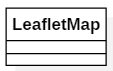
\includegraphics[width=0.5\linewidth]{images/view/classes/LeafletMap}
\end{figure} 
\subsubsection{Declaration}{
\begin{lstlisting}[frame=none]
public class LeafletMap
 extends View.Map.AbstractMap\end{lstlisting}
\subsubsection{Constructor summary}{
\begin{verse}
\hyperlink{View.Map.LeafletMap()}{{\bf LeafletMap()}} Default constructor\\
\end{verse}
}
\subsubsection{Constructors}{
\vskip -2em
\begin{itemize}
\item{ 
\index{LeafletMap()}
\hypertarget{View.Map.LeafletMap()}{{\bf  LeafletMap}\\}
\begin{lstlisting}[frame=none]
public LeafletMap()\end{lstlisting} %end signature
\begin{itemize}
\item{
{\bf  Description}

Default constructor
}
\end{itemize}
}%end item
\end{itemize}
}
\subsubsection{Members inherited from class AbstractMap }{
\texttt{View.Map.AbstractMap} {\small 
\refdefined{View.Map.AbstractMap}}
{\small 

\vskip -2em
\begin{itemize}
\item{\vskip -1.5ex 
\texttt{public void {\bf  addLayer}(\texttt{MapLayer} {\bf  layer})
}%end signature
}%end item
\item{\vskip -1.5ex 
\texttt{protected {\bf  dataset}}%end signature
}%end item
\item{\vskip -1.5ex 
\texttt{public void {\bf  displayLayer}(\texttt{MapLayer} {\bf  layer})
}%end signature
}%end item
\item{\vskip -1.5ex 
\texttt{public void {\bf  hideLayer}(\texttt{MapLayer} {\bf  layer})
}%end signature
}%end item
\item{\vskip -1.5ex 
\texttt{public void {\bf  mapOptionUpdate}()
}%end signature
}%end item
\item{\vskip -1.5ex 
\texttt{public void {\bf  notify}()
}%end signature
}%end item
\item{\vskip -1.5ex 
\texttt{protected {\bf  position}}%end signature
}%end item
\item{\vskip -1.5ex 
\texttt{public void {\bf  removeLayer}(\texttt{MapLayer} {\bf  layer})
}%end signature
}%end item
\item{\vskip -1.5ex 
\texttt{public void {\bf  sensorOptionUpdate}()
}%end signature
}%end item
\item{\vskip -1.5ex 
\texttt{public void {\bf  setPosition}(\texttt{Point} {\bf  point})
}%end signature
}%end item
\item{\vskip -1.5ex 
\texttt{public void {\bf  setTimeStamp}(\texttt{java.util.Date} {\bf  timeStamp})
}%end signature
}%end item
\item{\vskip -1.5ex 
\texttt{public void {\bf  setZoom}(\texttt{int} {\bf  zoom})
}%end signature
}%end item
\item{\vskip -1.5ex 
\texttt{public void {\bf  subscribeObserver}(\texttt{MapObserver} {\bf  observer})
}%end signature
}%end item
\item{\vskip -1.5ex 
\texttt{public void {\bf  timeOptionUpdate}()
}%end signature
}%end item
\item{\vskip -1.5ex 
\texttt{protected {\bf  timeStamp}}%end signature
}%end item
\item{\vskip -1.5ex 
\texttt{public void {\bf  unsubscribeObserver}(\texttt{MapObserver} {\bf  observer})
}%end signature
}%end item
\item{\vskip -1.5ex 
\texttt{public void {\bf  updateDataset}(\texttt{RequestCommand} {\bf  dataset})
}%end signature
}%end item
\item{\vskip -1.5ex 
\texttt{protected {\bf  zoom}}%end signature
}%end item
\end{itemize}
}
}
\subsection{\label{View.Map.MapLayer}Class MapLayer}{
\hypertarget{View.Map.MapLayer}{}\vskip .1in 
A map layer that can be displayed on an AbstractMap.\vskip .1in 
\begin{figure}[!hbp]
	\centering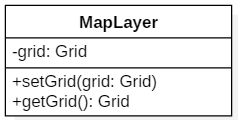
\includegraphics[width=0.5\linewidth]{images/view/classes/MapLayer}
\end{figure} 
\subsubsection{Declaration}{
\begin{lstlisting}[frame=none]
public class MapLayer
 extends java.lang.Object\end{lstlisting}
\subsubsection{Field summary}{
\begin{verse}
\hyperlink{View.Map.MapLayer.layers}{{\bf layers}} \\
\end{verse}
}
\subsubsection{Constructor summary}{
\begin{verse}
\hyperlink{View.Map.MapLayer()}{{\bf MapLayer()}} Default constructor\\
\end{verse}
}
\subsubsection{Method summary}{
\begin{verse}
\hyperlink{View.Map.MapLayer.getGrid()}{{\bf getGrid()}} Get the Grid of this MapLayer.\\
\hyperlink{View.Map.MapLayer.setGrid(Grid)}{{\bf setGrid(Grid)}} Set the grid of this MapLayer.\\
\end{verse}
}
\subsubsection{Fields}{
\begin{itemize}
\item{
\index{layers}
\label{View.Map.MapLayer.layers}\hypertarget{View.Map.MapLayer.layers}{\texttt{protected AbstractMap\ {\bf  layers}}
}
}
\end{itemize}
}
\subsubsection{Constructors}{
\vskip -2em
\begin{itemize}
\item{ 
\index{MapLayer()}
\hypertarget{View.Map.MapLayer()}{{\bf  MapLayer}\\}
\begin{lstlisting}[frame=none]
public MapLayer()\end{lstlisting} %end signature
\begin{itemize}
\item{
{\bf  Description}

Default constructor
}
\end{itemize}
}%end item
\end{itemize}
}
\subsubsection{Methods}{
\vskip -2em
\begin{itemize}
\item{ 
\index{getGrid()}
\hypertarget{View.Map.MapLayer.getGrid()}{{\bf  getGrid}\\}
\begin{lstlisting}[frame=none]
public Grid getGrid()\end{lstlisting} %end signature
\begin{itemize}
\item{
{\bf  Description}

Get the Grid of this MapLayer.
}
\item{{\bf  Returns} -- 
the Grid of this MapLayer. 
}%end item
\end{itemize}
}%end item
\item{ 
\index{setGrid(Grid)}
\hypertarget{View.Map.MapLayer.setGrid(Grid)}{{\bf  setGrid}\\}
\begin{lstlisting}[frame=none]
public void setGrid(Grid grid)\end{lstlisting} %end signature
\begin{itemize}
\item{
{\bf  Description}

Set the grid of this MapLayer.
}
\item{
{\bf  Parameters}
  \begin{itemize}
   \item{
\texttt{grid} -- }
  \end{itemize}
}%end item
\end{itemize}
}%end item
\end{itemize}
}
}
\subsection{\label{View.Map.MapOptionPanel}Class MapOptionPanel}{
\hypertarget{View.Map.MapOptionPanel}{}\vskip .1in 
An implementation of AbstractMapOptionPanel.\vskip .1in 
\begin{figure}[!hbp]
	\centering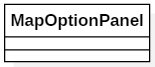
\includegraphics[width=0.5\linewidth]{images/view/classes/MapOptionPanel}
\end{figure} 
\subsubsection{Declaration}{
\begin{lstlisting}[frame=none]
public class MapOptionPanel
 extends View.Map.AbstractMapOptionPanel\end{lstlisting}
\subsubsection{Constructor summary}{
\begin{verse}
\hyperlink{View.Map.MapOptionPanel()}{{\bf MapOptionPanel()}} Default constructor\\
\end{verse}
}
\subsubsection{Constructors}{
\vskip -2em
\begin{itemize}
\item{ 
\index{MapOptionPanel()}
\hypertarget{View.Map.MapOptionPanel()}{{\bf  MapOptionPanel}\\}
\begin{lstlisting}[frame=none]
public MapOptionPanel()\end{lstlisting} %end signature
\begin{itemize}
\item{
{\bf  Description}

Default constructor
}
\end{itemize}
}%end item
\end{itemize}
}
\subsubsection{Members inherited from class AbstractMapOptionPanel }{
\texttt{View.Map.AbstractMapOptionPanel} {\small 
\refdefined{View.Map.AbstractMapOptionPanel}}
{\small 

\vskip -2em
\begin{itemize}
\item{\vskip -1.5ex 
\texttt{public Set {\bf  getTileTypes}()
}%end signature
}%end item
\item{\vskip -1.5ex 
\texttt{public void {\bf  notify}()
}%end signature
}%end item
\item{\vskip -1.5ex 
\texttt{protected {\bf  observers}}%end signature
}%end item
\item{\vskip -1.5ex 
\texttt{public void {\bf  setTileTypes}(\texttt{java.util.Set} {\bf  tileTypes})
}%end signature
}%end item
\item{\vskip -1.5ex 
\texttt{public void {\bf  subscribeObserver}(\texttt{MapOptionPanelObserver} {\bf  observer})
}%end signature
}%end item
\item{\vskip -1.5ex 
\texttt{public void {\bf  unsubscribeObserver}(\texttt{MapOptionPanelObserver} {\bf  observer})
}%end signature
}%end item
\end{itemize}
}
}
\subsection{\label{View.Map.TileType}Class TileType}{
\hypertarget{View.Map.TileType}{}\vskip .1in 
The type of a tile.\vskip .1in 
\begin{figure}[!hbp]
	\centering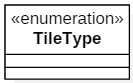
\includegraphics[width=0.5\linewidth]{images/view/classes/TileType}
\end{figure} 
\subsubsection{Declaration}{
\begin{lstlisting}[frame=none]
public class TileType
 extends java.lang.Object\end{lstlisting}
\subsubsection{Field summary}{
\begin{verse}
\hyperlink{View.Map.TileType.tileTypes}{{\bf tileTypes}} \\
\end{verse}
}
\subsubsection{Constructor summary}{
\begin{verse}
\hyperlink{View.Map.TileType()}{{\bf TileType()}} Default constructor\\
\end{verse}
}
\subsubsection{Fields}{
\begin{itemize}
\item{
\index{tileTypes}
\label{View.Map.TileType.tileTypes}\hypertarget{View.Map.TileType.tileTypes}{\texttt{protected AbstractMapOptionPanel\ {\bf  tileTypes}}
}
}
\end{itemize}
}
\subsubsection{Constructors}{
\vskip -2em
\begin{itemize}
\item{ 
\index{TileType()}
\hypertarget{View.Map.TileType()}{{\bf  TileType}\\}
\begin{lstlisting}[frame=none]
public TileType()\end{lstlisting} %end signature
\begin{itemize}
\item{
{\bf  Description}

Default constructor
}
\end{itemize}
}%end item
\end{itemize}
}
}
}
\section{Package View.SensorOption}{
\label{View.SensorOption}\hypertarget{View.SensorOption}{}
\hskip -.05in
\hbox to \hsize{\textit{ Package Contents\hfil Page}}
\vskip .13in
\hbox{{\bf  Interfaces}}
\entityintro{SensorOptionPanelObserver}{View.SensorOption.SensorOptionPanelObserver}{An observer that is meant to observe changes in the SensorOptionPanel.}
\vskip .13in
\hbox{{\bf  Classes}}
\entityintro{AbstractSensorOptionPanel}{View.SensorOption.AbstractSensorOptionPanel}{A panel for handling user input, that deals with setting a new ObservedProperty and notifying its observers about changes.}
\entityintro{ObservedProperty}{View.SensorOption.ObservedProperty}{The data type measured by a sensor.}
\entityintro{SensorOptionPanel}{View.SensorOption.SensorOptionPanel}{An implementation of AbstractSensorOptionPanel.}
\vskip .1in
\vskip .1in
\subsection{\label{View.SensorOption.SensorOptionPanelObserver}Interface SensorOptionPanelObserver}{
\hypertarget{View.SensorOption.SensorOptionPanelObserver}{}\vskip .1in 
An observer that is meant to observe changes in the SensorOptionPanel.\vskip .1in 
\begin{figure}[!hbp]
	\centering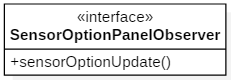
\includegraphics[width=0.5\linewidth]{images/view/classes/SensorOptionPanelObserver}
\end{figure} 
\subsubsection{Declaration}{
\begin{lstlisting}[frame=none]
public interface SensorOptionPanelObserver
\end{lstlisting}
\subsubsection{Method summary}{
\begin{verse}
\hyperlink{View.SensorOption.SensorOptionPanelObserver.sensorOptionUpdate()}{{\bf sensorOptionUpdate()}} Update the observer with the current SensorOptionPanel state.\\
\end{verse}
}
\subsubsection{Methods}{
\vskip -2em
\begin{itemize}
\item{ 
\index{sensorOptionUpdate()}
\hypertarget{View.SensorOption.SensorOptionPanelObserver.sensorOptionUpdate()}{{\bf  sensorOptionUpdate}\\}
\begin{lstlisting}[frame=none]
void sensorOptionUpdate()\end{lstlisting} %end signature
\begin{itemize}
\item{
{\bf  Description}

Update the observer with the current SensorOptionPanel state.
}
\end{itemize}
}%end item
\end{itemize}
}
}
\subsection{\label{View.SensorOption.AbstractSensorOptionPanel}Class AbstractSensorOptionPanel}{
\hypertarget{View.SensorOption.AbstractSensorOptionPanel}{}\vskip .1in 
A panel for handling user input, that deals with setting a new ObservedProperty and notifying its observers about changes.\vskip .1in 
\begin{figure}[!hbp]
	\centering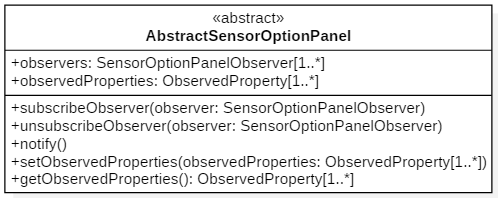
\includegraphics[width=0.5\linewidth]{images/view/classes/AbstractSensorOptionPanel}
\end{figure} 
\subsubsection{Declaration}{
\begin{lstlisting}[frame=none]
public class AbstractSensorOptionPanel
 extends ViewComponent\end{lstlisting}
\subsubsection{All known subclasses}{SensorOptionPanel\small{\refdefined{View.SensorOption.SensorOptionPanel}}}
\subsubsection{Constructor summary}{
\begin{verse}
\hyperlink{View.SensorOption.AbstractSensorOptionPanel()}{{\bf AbstractSensorOptionPanel()}} Default constructor\\
\end{verse}
}
\subsubsection{Method summary}{
\begin{verse}
\hyperlink{View.SensorOption.AbstractSensorOptionPanel.getObservedProperties()}{{\bf getObservedProperties()}} Get the sensor types.\\
\hyperlink{View.SensorOption.AbstractSensorOptionPanel.notify()}{{\bf notify()}} Notify all subscribed SensorOptionPanelObservers about a change in this AbstractSensorOptionPanel.\\
\hyperlink{View.SensorOption.AbstractSensorOptionPanel.setObservedProperties(java.util.Set)}{{\bf setObservedProperties(Set)}} Set the sensor types.\\
\hyperlink{View.SensorOption.AbstractSensorOptionPanel.subscribeObserver(View.SensorOption.SensorOptionPanelObserver)}{{\bf subscribeObserver(SensorOptionPanelObserver)}} Subscribe a SensorOptionPanelObserver to this AbstractSensorOptionPanel.\\
\hyperlink{View.SensorOption.AbstractSensorOptionPanel.unsubscribeObserver(View.SensorOption.SensorOptionPanelObserver)}{{\bf unsubscribeObserver(SensorOptionPanelObserver)}} Unsubscribe a SensorOptionPanelObserver from this AbstractSensorOptionPanel.\\
\end{verse}
}
\subsubsection{Constructors}{
\vskip -2em
\begin{itemize}
\item{ 
\index{AbstractSensorOptionPanel()}
\hypertarget{View.SensorOption.AbstractSensorOptionPanel()}{{\bf  AbstractSensorOptionPanel}\\}
\begin{lstlisting}[frame=none]
public AbstractSensorOptionPanel()\end{lstlisting} %end signature
\begin{itemize}
\item{
{\bf  Description}

Default constructor
}
\end{itemize}
}%end item
\end{itemize}
}
\subsubsection{Methods}{
\vskip -2em
\begin{itemize}
\item{ 
\index{getObservedProperties()}
\hypertarget{View.SensorOption.AbstractSensorOptionPanel.getObservedProperties()}{{\bf  getObservedProperties}\\}
\begin{lstlisting}[frame=none]
public java.util.Set getObservedProperties()\end{lstlisting} %end signature
\begin{itemize}
\item{
{\bf  Description}

Get the sensor types.
}
\item{{\bf  Returns} -- 
the sensor types. 
}%end item
\end{itemize}
}%end item
\item{ 
\index{notify()}
\hypertarget{View.SensorOption.AbstractSensorOptionPanel.notify()}{{\bf  notify}\\}
\begin{lstlisting}[frame=none]
public void notify()\end{lstlisting} %end signature
\begin{itemize}
\item{
{\bf  Description}

Notify all subscribed SensorOptionPanelObservers about a change in this AbstractSensorOptionPanel.
}
\end{itemize}
}%end item
\item{ 
\index{setObservedProperties(Set)}
\hypertarget{View.SensorOption.AbstractSensorOptionPanel.setObservedProperties(java.util.Set)}{{\bf  setObservedProperties}\\}
\begin{lstlisting}[frame=none]
public void setObservedProperties(java.util.Set observedProperties)\end{lstlisting} %end signature
\begin{itemize}
\item{
{\bf  Description}

Set the sensor types.
}
\item{
{\bf  Parameters}
  \begin{itemize}
   \item{
\texttt{observedProperties} -- }
  \end{itemize}
}%end item
\end{itemize}
}%end item
\item{ 
\index{subscribeObserver(SensorOptionPanelObserver)}
\hypertarget{View.SensorOption.AbstractSensorOptionPanel.subscribeObserver(View.SensorOption.SensorOptionPanelObserver)}{{\bf  subscribeObserver}\\}
\begin{lstlisting}[frame=none]
public void subscribeObserver(SensorOptionPanelObserver observer)\end{lstlisting} %end signature
\begin{itemize}
\item{
{\bf  Description}

Subscribe a SensorOptionPanelObserver to this AbstractSensorOptionPanel.
}
\item{
{\bf  Parameters}
  \begin{itemize}
   \item{
\texttt{observer} -- }
  \end{itemize}
}%end item
\end{itemize}
}%end item
\item{ 
\index{unsubscribeObserver(SensorOptionPanelObserver)}
\hypertarget{View.SensorOption.AbstractSensorOptionPanel.unsubscribeObserver(View.SensorOption.SensorOptionPanelObserver)}{{\bf  unsubscribeObserver}\\}
\begin{lstlisting}[frame=none]
public void unsubscribeObserver(SensorOptionPanelObserver observer)\end{lstlisting} %end signature
\begin{itemize}
\item{
{\bf  Description}

Unsubscribe a SensorOptionPanelObserver from this AbstractSensorOptionPanel.
}
\item{
{\bf  Parameters}
  \begin{itemize}
   \item{
\texttt{observer} -- }
  \end{itemize}
}%end item
\end{itemize}
}%end item
\end{itemize}
}
}
\subsection{\label{View.SensorOption.ObservedProperty}Class ObservedProperty}{
\hypertarget{View.SensorOption.ObservedProperty}{}\vskip .1in 
The data type measured by a sensor.\vskip .1in 
\begin{figure}[!hbp]
	\centering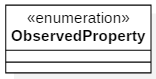
\includegraphics[width=0.5\linewidth]{images/view/classes/ObservedProperty}
\end{figure} 
\subsubsection{Declaration}{
\begin{lstlisting}[frame=none]
public class ObservedProperty
 extends java.lang.Object\end{lstlisting}
\subsubsection{Constructor summary}{
\begin{verse}
\hyperlink{View.SensorOption.ObservedProperty()}{{\bf ObservedProperty()}} Default constructor\\
\end{verse}
}
\subsubsection{Constructors}{
\vskip -2em
\begin{itemize}
\item{ 
\index{ObservedProperty()}
\hypertarget{View.SensorOption.ObservedProperty()}{{\bf  ObservedProperty}\\}
\begin{lstlisting}[frame=none]
public ObservedProperty()\end{lstlisting} %end signature
\begin{itemize}
\item{
{\bf  Description}

Default constructor
}
\end{itemize}
}%end item
\end{itemize}
}
}
\subsection{\label{View.SensorOption.SensorOptionPanel}Class SensorOptionPanel}{
\hypertarget{View.SensorOption.SensorOptionPanel}{}\vskip .1in 
An implementation of AbstractSensorOptionPanel.\vskip .1in 
\begin{figure}[!hbp]
	\centering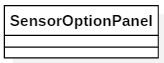
\includegraphics[width=0.5\linewidth]{images/view/classes/SensorOptionPanel}
\end{figure} 
\subsubsection{Declaration}{
\begin{lstlisting}[frame=none]
public class SensorOptionPanel
 extends View.SensorOption.AbstractSensorOptionPanel\end{lstlisting}
\subsubsection{Constructor summary}{
\begin{verse}
\hyperlink{View.SensorOption.SensorOptionPanel()}{{\bf SensorOptionPanel()}} Default constructor\\
\end{verse}
}
\subsubsection{Constructors}{
\vskip -2em
\begin{itemize}
\item{ 
\index{SensorOptionPanel()}
\hypertarget{View.SensorOption.SensorOptionPanel()}{{\bf  SensorOptionPanel}\\}
\begin{lstlisting}[frame=none]
public SensorOptionPanel()\end{lstlisting} %end signature
\begin{itemize}
\item{
{\bf  Description}

Default constructor
}
\end{itemize}
}%end item
\end{itemize}
}
\subsubsection{Members inherited from class AbstractSensorOptionPanel }{
\texttt{View.SensorOption.AbstractSensorOptionPanel} {\small 
\refdefined{View.SensorOption.AbstractSensorOptionPanel}}
{\small 

\vskip -2em
\begin{itemize}
\item{\vskip -1.5ex 
\texttt{public Set {\bf  getObservedProperties}()
}%end signature
}%end item
\item{\vskip -1.5ex 
\texttt{public void {\bf  notify}()
}%end signature
}%end item
\item{\vskip -1.5ex 
\texttt{public void {\bf  setObservedProperties}(\texttt{java.util.Set} {\bf  observedProperties})
}%end signature
}%end item
\item{\vskip -1.5ex 
\texttt{public void {\bf  subscribeObserver}(\texttt{SensorOptionPanelObserver} {\bf  observer})
}%end signature
}%end item
\item{\vskip -1.5ex 
\texttt{public void {\bf  unsubscribeObserver}(\texttt{SensorOptionPanelObserver} {\bf  observer})
}%end signature
}%end item
\end{itemize}
}
}
}
\section{Package View.SensorTable}{
\label{View.SensorTable}\hypertarget{View.SensorTable}{}
\hskip -.05in
\hbox to \hsize{\textit{ Package Contents\hfil Page}}
\vskip .13in
\hbox{{\bf  Classes}}
\entityintro{AbstractSensorTable}{View.SensorTable.AbstractSensorTable}{A table that visualizes the data in its dataset and enables the selection of a Sensor by using its SensorID.}
\entityintro{SensorTable}{View.SensorTable.SensorTable}{An implementation of AbstractSensorTable.}
\vskip .1in
\vskip .1in
\subsection{\label{View.SensorTable.AbstractSensorTable}Class AbstractSensorTable}{
\hypertarget{View.SensorTable.AbstractSensorTable}{}\vskip .1in 
A table that visualizes the data in its dataset and enables the selection of a Sensor by using its SensorID.\vskip .1in 
\begin{figure}[!hbp]
	\centering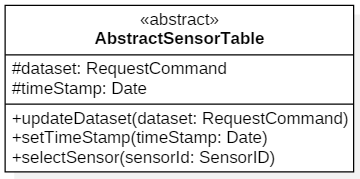
\includegraphics[width=0.5\linewidth]{images/view/classes/AbstractSensorTable}
\end{figure} 
\subsubsection{Declaration}{
\begin{lstlisting}[frame=none]
public class AbstractSensorTable
 extends ViewComponent\end{lstlisting}
\subsubsection{All known subclasses}{SensorTable\small{\refdefined{View.SensorTable.SensorTable}}}
\subsubsection{Field summary}{
\begin{verse}
\hyperlink{View.SensorTable.AbstractSensorTable.dataset}{{\bf dataset}} \\
\hyperlink{View.SensorTable.AbstractSensorTable.timeStamp}{{\bf timeStamp}} \\
\end{verse}
}
\subsubsection{Constructor summary}{
\begin{verse}
\hyperlink{View.SensorTable.AbstractSensorTable()}{{\bf AbstractSensorTable()}} Default constructor\\
\end{verse}
}
\subsubsection{Method summary}{
\begin{verse}
\hyperlink{View.SensorTable.AbstractSensorTable.mapUpdate()}{{\bf mapUpdate()}} \\
\hyperlink{View.SensorTable.AbstractSensorTable.selectSensor(SensorID)}{{\bf selectSensor(SensorID)}} Select a sensor in the dataset by using its SensorID.\\
\hyperlink{View.SensorTable.AbstractSensorTable.sensorOptionUpdate()}{{\bf sensorOptionUpdate()}} Update the observer with the current SensorOptionPanel state.\\
\hyperlink{View.SensorTable.AbstractSensorTable.setTimeStamp(java.util.Date)}{{\bf setTimeStamp(Date)}} Set a time stamp and display the data from the dataset at the specified point in time.\\
\hyperlink{View.SensorTable.AbstractSensorTable.timeOptionUpdate()}{{\bf timeOptionUpdate()}} Update the observer with the current TimeOptionPanel state.\\
\hyperlink{View.SensorTable.AbstractSensorTable.updateDataset(RequestCommand)}{{\bf updateDataset(RequestCommand)}} Update the dataset of this AbstractSensorTable by giving it a new RequestCommand.\\
\end{verse}
}
\subsubsection{Fields}{
\begin{itemize}
\item{
\index{dataset}
\label{View.SensorTable.AbstractSensorTable.dataset}\hypertarget{View.SensorTable.AbstractSensorTable.dataset}{\texttt{protected RequestCommand\ {\bf  dataset}}
}
}
\item{
\index{timeStamp}
\label{View.SensorTable.AbstractSensorTable.timeStamp}\hypertarget{View.SensorTable.AbstractSensorTable.timeStamp}{\texttt{protected java.util.Date\ {\bf  timeStamp}}
}
}
\end{itemize}
}
\subsubsection{Constructors}{
\vskip -2em
\begin{itemize}
\item{ 
\index{AbstractSensorTable()}
\hypertarget{View.SensorTable.AbstractSensorTable()}{{\bf  AbstractSensorTable}\\}
\begin{lstlisting}[frame=none]
public AbstractSensorTable()\end{lstlisting} %end signature
\begin{itemize}
\item{
{\bf  Description}

Default constructor
}
\end{itemize}
}%end item
\end{itemize}
}
\subsubsection{Methods}{
\vskip -2em
\begin{itemize}
\item{ 
\index{mapUpdate()}
\hypertarget{View.SensorTable.AbstractSensorTable.mapUpdate()}{{\bf  mapUpdate}\\}
\begin{lstlisting}[frame=none]
public void mapUpdate()\end{lstlisting} %end signature
}%end item
\item{ 
\index{selectSensor(SensorID)}
\hypertarget{View.SensorTable.AbstractSensorTable.selectSensor(SensorID)}{{\bf  selectSensor}\\}
\begin{lstlisting}[frame=none]
public void selectSensor(SensorID sensorId)\end{lstlisting} %end signature
\begin{itemize}
\item{
{\bf  Description}

Select a sensor in the dataset by using its SensorID.
}
\item{
{\bf  Parameters}
  \begin{itemize}
   \item{
\texttt{sensorId} -- }
  \end{itemize}
}%end item
\end{itemize}
}%end item
\item{ 
\index{sensorOptionUpdate()}
\hypertarget{View.SensorTable.AbstractSensorTable.sensorOptionUpdate()}{{\bf  sensorOptionUpdate}\\}
\begin{lstlisting}[frame=none]
public void sensorOptionUpdate()\end{lstlisting} %end signature
\begin{itemize}
\item{
{\bf  Description}

Update the observer with the current SensorOptionPanel state.
}
\end{itemize}
}%end item
\item{ 
\index{setTimeStamp(Date)}
\hypertarget{View.SensorTable.AbstractSensorTable.setTimeStamp(java.util.Date)}{{\bf  setTimeStamp}\\}
\begin{lstlisting}[frame=none]
public void setTimeStamp(java.util.Date timeStamp)\end{lstlisting} %end signature
\begin{itemize}
\item{
{\bf  Description}

Set a time stamp and display the data from the dataset at the specified point in time.
}
\item{
{\bf  Parameters}
  \begin{itemize}
   \item{
\texttt{timeStamp} -- }
  \end{itemize}
}%end item
\end{itemize}
}%end item
\item{ 
\index{timeOptionUpdate()}
\hypertarget{View.SensorTable.AbstractSensorTable.timeOptionUpdate()}{{\bf  timeOptionUpdate}\\}
\begin{lstlisting}[frame=none]
public void timeOptionUpdate()\end{lstlisting} %end signature
\begin{itemize}
\item{
{\bf  Description}

Update the observer with the current TimeOptionPanel state.
}
\end{itemize}
}%end item
\item{ 
\index{updateDataset(RequestCommand)}
\hypertarget{View.SensorTable.AbstractSensorTable.updateDataset(RequestCommand)}{{\bf  updateDataset}\\}
\begin{lstlisting}[frame=none]
public void updateDataset(RequestCommand dataset)\end{lstlisting} %end signature
\begin{itemize}
\item{
{\bf  Description}

Update the dataset of this AbstractSensorTable by giving it a new RequestCommand.
}
\item{
{\bf  Parameters}
  \begin{itemize}
   \item{
\texttt{dataset} -- }
  \end{itemize}
}%end item
\end{itemize}
}%end item
\end{itemize}
}
}
\subsection{\label{View.SensorTable.SensorTable}Class SensorTable}{
\hypertarget{View.SensorTable.SensorTable}{}\vskip .1in 
An implementation of AbstractSensorTable.\vskip .1in 
\begin{figure}[!hbp]
	\centering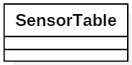
\includegraphics[width=0.5\linewidth]{images/view/classes/SensorTable}
\end{figure} 
\subsubsection{Declaration}{
\begin{lstlisting}[frame=none]
public class SensorTable
 extends View.SensorTable.AbstractSensorTable\end{lstlisting}
\subsubsection{Constructor summary}{
\begin{verse}
\hyperlink{View.SensorTable.SensorTable()}{{\bf SensorTable()}} Default constructor\\
\end{verse}
}
\subsubsection{Constructors}{
\vskip -2em
\begin{itemize}
\item{ 
\index{SensorTable()}
\hypertarget{View.SensorTable.SensorTable()}{{\bf  SensorTable}\\}
\begin{lstlisting}[frame=none]
public SensorTable()\end{lstlisting} %end signature
\begin{itemize}
\item{
{\bf  Description}

Default constructor
}
\end{itemize}
}%end item
\end{itemize}
}
\subsubsection{Members inherited from class AbstractSensorTable }{
\texttt{View.SensorTable.AbstractSensorTable} {\small 
\refdefined{View.SensorTable.AbstractSensorTable}}
{\small 

\vskip -2em
\begin{itemize}
\item{\vskip -1.5ex 
\texttt{protected {\bf  dataset}}%end signature
}%end item
\item{\vskip -1.5ex 
\texttt{public void {\bf  mapUpdate}()
}%end signature
}%end item
\item{\vskip -1.5ex 
\texttt{public void {\bf  selectSensor}(\texttt{SensorID} {\bf  sensorId})
}%end signature
}%end item
\item{\vskip -1.5ex 
\texttt{public void {\bf  sensorOptionUpdate}()
}%end signature
}%end item
\item{\vskip -1.5ex 
\texttt{public void {\bf  setTimeStamp}(\texttt{java.util.Date} {\bf  timeStamp})
}%end signature
}%end item
\item{\vskip -1.5ex 
\texttt{public void {\bf  timeOptionUpdate}()
}%end signature
}%end item
\item{\vskip -1.5ex 
\texttt{protected {\bf  timeStamp}}%end signature
}%end item
\item{\vskip -1.5ex 
\texttt{public void {\bf  updateDataset}(\texttt{RequestCommand} {\bf  dataset})
}%end signature
}%end item
\end{itemize}
}
}
}
\section{Package View.TimeOption}{
\label{View.TimeOption}\hypertarget{View.TimeOption}{}
\hskip -.05in
\hbox to \hsize{\textit{ Package Contents\hfil Page}}
\vskip .13in
\hbox{{\bf  Interfaces}}
\entityintro{TimeOptionPanelObserver}{View.TimeOption.TimeOptionPanelObserver}{An observer that is meant to observe changes in the TimeOptionPanel.}
\vskip .13in
\hbox{{\bf  Classes}}
\entityintro{AbstractTimeOptionPanel}{View.TimeOption.AbstractTimeOptionPanel}{A panel for handling user input, that deals with timing options and notifying its observers about changes in its state.}
\entityintro{HistoricalRefreshState}{View.TimeOption.HistoricalRefreshState}{In this state the refresh function simulates the historical data mode.}
\entityintro{LiveRefreshState}{View.TimeOption.LiveRefreshState}{In this state the refresh function simulates the live data mode.}
\entityintro{LoopRefreshState}{View.TimeOption.LoopRefreshState}{In this state the refresh function simulates the loop data mode.}
\entityintro{RefreshConfiguration}{View.TimeOption.RefreshConfiguration}{Encapsulates the preferences about the fetching of live data and the loop mode of historical data.}
\entityintro{RefreshContext}{View.TimeOption.RefreshContext}{Encapsulates the logic of switching between historical and live data mode and starting and stopping the loop mode.}
\entityintro{RefreshState}{View.TimeOption.RefreshState}{A state}
\entityintro{TimeOptionPanel}{View.TimeOption.TimeOptionPanel}{An implementation of AbstractTimeOptionPanel.}
\vskip .1in
\vskip .1in
\subsection{\label{View.TimeOption.TimeOptionPanelObserver}Interface TimeOptionPanelObserver}{
\hypertarget{View.TimeOption.TimeOptionPanelObserver}{}\vskip .1in 
An observer that is meant to observe changes in the TimeOptionPanel.\vskip .1in 
\begin{figure}[!hbp]
	\centering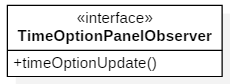
\includegraphics[width=0.5\linewidth]{images/view/classes/TimeOptionPanelObserver}
\end{figure} 
\subsubsection{Declaration}{
\begin{lstlisting}[frame=none]
public interface TimeOptionPanelObserver
\end{lstlisting}
\subsubsection{All known subinterfaces}{RefreshContext\small{\refdefined{View.TimeOption.RefreshContext}}}
\subsubsection{All classes known to implement interface}{RefreshContext\small{\refdefined{View.TimeOption.RefreshContext}}}
\subsubsection{Method summary}{
\begin{verse}
\hyperlink{View.TimeOption.TimeOptionPanelObserver.timeOptionUpdate()}{{\bf timeOptionUpdate()}} Update the observer with the current TimeOptionPanel state.\\
\end{verse}
}
\subsubsection{Methods}{
\vskip -2em
\begin{itemize}
\item{ 
\index{timeOptionUpdate()}
\hypertarget{View.TimeOption.TimeOptionPanelObserver.timeOptionUpdate()}{{\bf  timeOptionUpdate}\\}
\begin{lstlisting}[frame=none]
void timeOptionUpdate()\end{lstlisting} %end signature
\begin{itemize}
\item{
{\bf  Description}

Update the observer with the current TimeOptionPanel state.
}
\end{itemize}
}%end item
\end{itemize}
}
}
\subsection{\label{View.TimeOption.AbstractTimeOptionPanel}Class AbstractTimeOptionPanel}{
\hypertarget{View.TimeOption.AbstractTimeOptionPanel}{}\vskip .1in 
A panel for handling user input, that deals with timing options and notifying its observers about changes in its state.\vskip .1in 
\begin{figure}[!hbp]
	\centering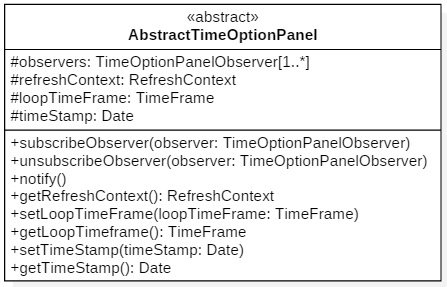
\includegraphics[width=0.5\linewidth]{images/view/classes/AbstractTimeOptionPanel}
\end{figure} 
\subsubsection{Declaration}{
\begin{lstlisting}[frame=none]
public class AbstractTimeOptionPanel
 extends ViewComponent\end{lstlisting}
\subsubsection{All known subclasses}{TimeOptionPanel\small{\refdefined{View.TimeOption.TimeOptionPanel}}}
\subsubsection{Field summary}{
\begin{verse}
\hyperlink{View.TimeOption.AbstractTimeOptionPanel.loopTimeFrame}{{\bf loopTimeFrame}} \\
\hyperlink{View.TimeOption.AbstractTimeOptionPanel.refreshConfig}{{\bf refreshConfig}} \\
\hyperlink{View.TimeOption.AbstractTimeOptionPanel.timeStamp}{{\bf timeStamp}} \\
\end{verse}
}
\subsubsection{Constructor summary}{
\begin{verse}
\hyperlink{View.TimeOption.AbstractTimeOptionPanel()}{{\bf AbstractTimeOptionPanel()}} Default constructor\\
\end{verse}
}
\subsubsection{Method summary}{
\begin{verse}
\hyperlink{View.TimeOption.AbstractTimeOptionPanel.getLoopTimeframe()}{{\bf getLoopTimeframe()}} Get the loop time frame.\\
\hyperlink{View.TimeOption.AbstractTimeOptionPanel.getRefreshContext()}{{\bf getRefreshContext()}} Get the RefreshContext.\\
\hyperlink{View.TimeOption.AbstractTimeOptionPanel.getTimeStamp()}{{\bf getTimeStamp()}} Get the time stamp.\\
\hyperlink{View.TimeOption.AbstractTimeOptionPanel.notify()}{{\bf notify()}} Notify all subscribed TimeOptionPanelObservers about a change in this AbstractTimeOptionPanel.\\
\hyperlink{View.TimeOption.AbstractTimeOptionPanel.setLoopTimeFrame(TimeFrame)}{{\bf setLoopTimeFrame(TimeFrame)}} Set the start and end time point of the loop.\\
\hyperlink{View.TimeOption.AbstractTimeOptionPanel.setTimeStamp(java.util.Date)}{{\bf setTimeStamp(Date)}} Set the time stamp.\\
\hyperlink{View.TimeOption.AbstractTimeOptionPanel.subscribeObserver(View.TimeOption.TimeOptionPanelObserver)}{{\bf subscribeObserver(TimeOptionPanelObserver)}} Subscribe a TimeOptionPanelObserver to this AbstractTimeOptionPanel.\\
\hyperlink{View.TimeOption.AbstractTimeOptionPanel.unsubscribeObserver(View.TimeOption.TimeOptionPanelObserver)}{{\bf unsubscribeObserver(TimeOptionPanelObserver)}} Unsubscribe a TimeOptionPanelObserver from this AbstractTimeOptionPanel.\\
\end{verse}
}
\subsubsection{Fields}{
\begin{itemize}
\item{
\index{loopTimeFrame}
\label{View.TimeOption.AbstractTimeOptionPanel.loopTimeFrame}\hypertarget{View.TimeOption.AbstractTimeOptionPanel.loopTimeFrame}{\texttt{protected TimeFrame\ {\bf  loopTimeFrame}}
}
}
\item{
\index{timeStamp}
\label{View.TimeOption.AbstractTimeOptionPanel.timeStamp}\hypertarget{View.TimeOption.AbstractTimeOptionPanel.timeStamp}{\texttt{protected java.util.Date\ {\bf  timeStamp}}
}
}
\item{
\index{refreshConfig}
\label{View.TimeOption.AbstractTimeOptionPanel.refreshConfig}\hypertarget{View.TimeOption.AbstractTimeOptionPanel.refreshConfig}{\texttt{protected RefreshConfiguration\ {\bf  refreshConfig}}
}
}
\end{itemize}
}
\subsubsection{Constructors}{
\vskip -2em
\begin{itemize}
\item{ 
\index{AbstractTimeOptionPanel()}
\hypertarget{View.TimeOption.AbstractTimeOptionPanel()}{{\bf  AbstractTimeOptionPanel}\\}
\begin{lstlisting}[frame=none]
public AbstractTimeOptionPanel()\end{lstlisting} %end signature
\begin{itemize}
\item{
{\bf  Description}

Default constructor
}
\end{itemize}
}%end item
\end{itemize}
}
\subsubsection{Methods}{
\vskip -2em
\begin{itemize}
\item{ 
\index{getLoopTimeframe()}
\hypertarget{View.TimeOption.AbstractTimeOptionPanel.getLoopTimeframe()}{{\bf  getLoopTimeframe}\\}
\begin{lstlisting}[frame=none]
public TimeFrame getLoopTimeframe()\end{lstlisting} %end signature
\begin{itemize}
\item{
{\bf  Description}

Get the loop time frame.
}
\item{{\bf  Returns} -- 
the loop time frame. 
}%end item
\end{itemize}
}%end item
\item{ 
\index{getRefreshContext()}
\hypertarget{View.TimeOption.AbstractTimeOptionPanel.getRefreshContext()}{{\bf  getRefreshContext}\\}
\begin{lstlisting}[frame=none]
public RefreshContext getRefreshContext()\end{lstlisting} %end signature
\begin{itemize}
\item{
{\bf  Description}

Get the RefreshContext.
}
\item{{\bf  Returns} -- 
the RefreshContext. 
}%end item
\end{itemize}
}%end item
\item{ 
\index{getTimeStamp()}
\hypertarget{View.TimeOption.AbstractTimeOptionPanel.getTimeStamp()}{{\bf  getTimeStamp}\\}
\begin{lstlisting}[frame=none]
public java.util.Date getTimeStamp()\end{lstlisting} %end signature
\begin{itemize}
\item{
{\bf  Description}

Get the time stamp.
}
\item{{\bf  Returns} -- 
the time stamp. 
}%end item
\end{itemize}
}%end item
\item{ 
\index{notify()}
\hypertarget{View.TimeOption.AbstractTimeOptionPanel.notify()}{{\bf  notify}\\}
\begin{lstlisting}[frame=none]
public void notify()\end{lstlisting} %end signature
\begin{itemize}
\item{
{\bf  Description}

Notify all subscribed TimeOptionPanelObservers about a change in this AbstractTimeOptionPanel.
}
\end{itemize}
}%end item
\item{ 
\index{setLoopTimeFrame(TimeFrame)}
\hypertarget{View.TimeOption.AbstractTimeOptionPanel.setLoopTimeFrame(TimeFrame)}{{\bf  setLoopTimeFrame}\\}
\begin{lstlisting}[frame=none]
public void setLoopTimeFrame(TimeFrame loopTimeFrame)\end{lstlisting} %end signature
\begin{itemize}
\item{
{\bf  Description}

Set the start and end time point of the loop.
}
\item{
{\bf  Parameters}
  \begin{itemize}
   \item{
\texttt{loopTimeFrame} -- }
  \end{itemize}
}%end item
\end{itemize}
}%end item
\item{ 
\index{setTimeStamp(Date)}
\hypertarget{View.TimeOption.AbstractTimeOptionPanel.setTimeStamp(java.util.Date)}{{\bf  setTimeStamp}\\}
\begin{lstlisting}[frame=none]
public void setTimeStamp(java.util.Date timeStamp)\end{lstlisting} %end signature
\begin{itemize}
\item{
{\bf  Description}

Set the time stamp.
}
\item{
{\bf  Parameters}
  \begin{itemize}
   \item{
\texttt{timeStamp} -- }
  \end{itemize}
}%end item
\end{itemize}
}%end item
\item{ 
\index{subscribeObserver(TimeOptionPanelObserver)}
\hypertarget{View.TimeOption.AbstractTimeOptionPanel.subscribeObserver(View.TimeOption.TimeOptionPanelObserver)}{{\bf  subscribeObserver}\\}
\begin{lstlisting}[frame=none]
public void subscribeObserver(TimeOptionPanelObserver observer)\end{lstlisting} %end signature
\begin{itemize}
\item{
{\bf  Description}

Subscribe a TimeOptionPanelObserver to this AbstractTimeOptionPanel.
}
\item{
{\bf  Parameters}
  \begin{itemize}
   \item{
\texttt{observer} -- }
  \end{itemize}
}%end item
\end{itemize}
}%end item
\item{ 
\index{unsubscribeObserver(TimeOptionPanelObserver)}
\hypertarget{View.TimeOption.AbstractTimeOptionPanel.unsubscribeObserver(View.TimeOption.TimeOptionPanelObserver)}{{\bf  unsubscribeObserver}\\}
\begin{lstlisting}[frame=none]
public void unsubscribeObserver(TimeOptionPanelObserver observer)\end{lstlisting} %end signature
\begin{itemize}
\item{
{\bf  Description}

Unsubscribe a TimeOptionPanelObserver from this AbstractTimeOptionPanel.
}
\item{
{\bf  Parameters}
  \begin{itemize}
   \item{
\texttt{observer} -- }
  \end{itemize}
}%end item
\end{itemize}
}%end item
\end{itemize}
}
}
\subsection{\label{View.TimeOption.HistoricalRefreshState}Class HistoricalRefreshState}{
\hypertarget{View.TimeOption.HistoricalRefreshState}{}\vskip .1in 
In this state the refresh function simulates the historical data mode. The timeStamp parameter isn't altered and the currently selected dataset entries stay the same.\vskip .1in 
\begin{figure}[!hbp]
	\centering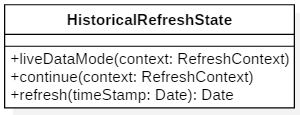
\includegraphics[width=0.5\linewidth]{images/view/classes/HistoricalRefreshState}
\end{figure} 
\subsubsection{Declaration}{
\begin{lstlisting}[frame=none]
public class HistoricalRefreshState
 extends View.TimeOption.RefreshState\end{lstlisting}
\subsubsection{Constructor summary}{
\begin{verse}
\hyperlink{View.TimeOption.HistoricalRefreshState()}{{\bf HistoricalRefreshState()}} Default constructor\\
\end{verse}
}
\subsubsection{Method summary}{
\begin{verse}
\hyperlink{View.TimeOption.HistoricalRefreshState.continueRoutine(View.TimeOption.RefreshContext)}{{\bf continueRoutine(RefreshContext)}} Switch to loop mode.\\
\hyperlink{View.TimeOption.HistoricalRefreshState.liveDataMode(View.TimeOption.RefreshContext)}{{\bf liveDataMode(RefreshContext)}} Switch to live data mode.\\
\hyperlink{View.TimeOption.HistoricalRefreshState.refresh(java.util.Date)}{{\bf refresh(Date)}} Returns the submitted time stamp without any change.\\
\end{verse}
}
\subsubsection{Constructors}{
\vskip -2em
\begin{itemize}
\item{ 
\index{HistoricalRefreshState()}
\hypertarget{View.TimeOption.HistoricalRefreshState()}{{\bf  HistoricalRefreshState}\\}
\begin{lstlisting}[frame=none]
public HistoricalRefreshState()\end{lstlisting} %end signature
\begin{itemize}
\item{
{\bf  Description}

Default constructor
}
\end{itemize}
}%end item
\end{itemize}
}
\subsubsection{Methods}{
\vskip -2em
\begin{itemize}
\item{ 
\index{continueRoutine(RefreshContext)}
\hypertarget{View.TimeOption.HistoricalRefreshState.continueRoutine(View.TimeOption.RefreshContext)}{{\bf  continueRoutine}\\}
\begin{lstlisting}[frame=none]
public void continueRoutine(RefreshContext context)\end{lstlisting} %end signature
\begin{itemize}
\item{
{\bf  Description}

Switch to loop mode.
}
\item{
{\bf  Parameters}
  \begin{itemize}
   \item{
\texttt{context} -- }
  \end{itemize}
}%end item
\end{itemize}
}%end item
\item{ 
\index{liveDataMode(RefreshContext)}
\hypertarget{View.TimeOption.HistoricalRefreshState.liveDataMode(View.TimeOption.RefreshContext)}{{\bf  liveDataMode}\\}
\begin{lstlisting}[frame=none]
public void liveDataMode(RefreshContext context)\end{lstlisting} %end signature
\begin{itemize}
\item{
{\bf  Description}

Switch to live data mode.
}
\item{
{\bf  Parameters}
  \begin{itemize}
   \item{
\texttt{context} -- }
  \end{itemize}
}%end item
\end{itemize}
}%end item
\item{ 
\index{refresh(Date)}
\hypertarget{View.TimeOption.HistoricalRefreshState.refresh(java.util.Date)}{{\bf  refresh}\\}
\begin{lstlisting}[frame=none]
public java.util.Date refresh(java.util.Date timeStamp)\end{lstlisting} %end signature
\begin{itemize}
\item{
{\bf  Description}

Returns the submitted time stamp without any change.
}
\item{
{\bf  Parameters}
  \begin{itemize}
   \item{
\texttt{timeStamp} -- }
  \end{itemize}
}%end item
\item{{\bf  Returns} -- 
the submitted time stamp without any change. 
}%end item
\end{itemize}
}%end item
\end{itemize}
}
\subsubsection{Members inherited from class RefreshState }{
\texttt{View.TimeOption.RefreshState} {\small 
\refdefined{View.TimeOption.RefreshState}}
{\small 

\vskip -2em
\begin{itemize}
\item{\vskip -1.5ex 
\texttt{public void {\bf  continueRoutine}(\texttt{RefreshContext} {\bf  context})
}%end signature
}%end item
\item{\vskip -1.5ex 
\texttt{public void {\bf  historicalDataMode}(\texttt{RefreshContext} {\bf  context})
}%end signature
}%end item
\item{\vskip -1.5ex 
\texttt{public void {\bf  liveDataMode}(\texttt{RefreshContext} {\bf  context})
}%end signature
}%end item
\item{\vskip -1.5ex 
\texttt{public Date {\bf  refresh}(\texttt{java.util.Date} {\bf  timeStamp})
}%end signature
}%end item
\item{\vskip -1.5ex 
\texttt{public void {\bf  stopRoutine}(\texttt{RefreshContext} {\bf  context})
}%end signature
}%end item
\end{itemize}
}
}
\subsection{\label{View.TimeOption.LiveRefreshState}Class LiveRefreshState}{
\hypertarget{View.TimeOption.LiveRefreshState}{}\vskip .1in 
In this state the refresh function simulates the live data mode. Depending on the RefreshConfiguration the refresh function fetches live data. The timeStamp parameter isn't altered.\vskip .1in 
\begin{figure}[!hbp]
	\centering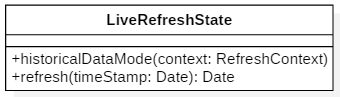
\includegraphics[width=0.5\linewidth]{images/view/classes/LiveRefreshState}
\end{figure} 
\subsubsection{Declaration}{
\begin{lstlisting}[frame=none]
public class LiveRefreshState
 extends View.TimeOption.RefreshState\end{lstlisting}
\subsubsection{Constructor summary}{
\begin{verse}
\hyperlink{View.TimeOption.LiveRefreshState()}{{\bf LiveRefreshState()}} Default constructor\\
\end{verse}
}
\subsubsection{Method summary}{
\begin{verse}
\hyperlink{View.TimeOption.LiveRefreshState.historicalDataMode(View.TimeOption.RefreshContext)}{{\bf historicalDataMode(RefreshContext)}} Switch to historical data mode.\\
\hyperlink{View.TimeOption.LiveRefreshState.refresh(java.util.Date)}{{\bf refresh(Date)}} Fetch live data and return the most up-to-date time stamp.\\
\end{verse}
}
\subsubsection{Constructors}{
\vskip -2em
\begin{itemize}
\item{ 
\index{LiveRefreshState()}
\hypertarget{View.TimeOption.LiveRefreshState()}{{\bf  LiveRefreshState}\\}
\begin{lstlisting}[frame=none]
public LiveRefreshState()\end{lstlisting} %end signature
\begin{itemize}
\item{
{\bf  Description}

Default constructor
}
\end{itemize}
}%end item
\end{itemize}
}
\subsubsection{Methods}{
\vskip -2em
\begin{itemize}
\item{ 
\index{historicalDataMode(RefreshContext)}
\hypertarget{View.TimeOption.LiveRefreshState.historicalDataMode(View.TimeOption.RefreshContext)}{{\bf  historicalDataMode}\\}
\begin{lstlisting}[frame=none]
public void historicalDataMode(RefreshContext context)\end{lstlisting} %end signature
\begin{itemize}
\item{
{\bf  Description}

Switch to historical data mode.
}
\item{
{\bf  Parameters}
  \begin{itemize}
   \item{
\texttt{context} -- }
  \end{itemize}
}%end item
\end{itemize}
}%end item
\item{ 
\index{refresh(Date)}
\hypertarget{View.TimeOption.LiveRefreshState.refresh(java.util.Date)}{{\bf  refresh}\\}
\begin{lstlisting}[frame=none]
public java.util.Date refresh(java.util.Date timeStamp)\end{lstlisting} %end signature
\begin{itemize}
\item{
{\bf  Description}

Fetch live data and return the most up-to-date time stamp.
}
\item{
{\bf  Parameters}
  \begin{itemize}
   \item{
\texttt{timeStamp} -- }
  \end{itemize}
}%end item
\item{{\bf  Returns} -- 
the most up-to-date time stamp. 
}%end item
\end{itemize}
}%end item
\end{itemize}
}
\subsubsection{Members inherited from class RefreshState }{
\texttt{View.TimeOption.RefreshState} {\small 
\refdefined{View.TimeOption.RefreshState}}
{\small 

\vskip -2em
\begin{itemize}
\item{\vskip -1.5ex 
\texttt{public void {\bf  continueRoutine}(\texttt{RefreshContext} {\bf  context})
}%end signature
}%end item
\item{\vskip -1.5ex 
\texttt{public void {\bf  historicalDataMode}(\texttt{RefreshContext} {\bf  context})
}%end signature
}%end item
\item{\vskip -1.5ex 
\texttt{public void {\bf  liveDataMode}(\texttt{RefreshContext} {\bf  context})
}%end signature
}%end item
\item{\vskip -1.5ex 
\texttt{public Date {\bf  refresh}(\texttt{java.util.Date} {\bf  timeStamp})
}%end signature
}%end item
\item{\vskip -1.5ex 
\texttt{public void {\bf  stopRoutine}(\texttt{RefreshContext} {\bf  context})
}%end signature
}%end item
\end{itemize}
}
}
\subsection{\label{View.TimeOption.LoopRefreshState}Class LoopRefreshState}{
\hypertarget{View.TimeOption.LoopRefreshState}{}\vskip .1in 
In this state the refresh function simulates the loop data mode. Depending on the loopTimeFrame value and the RefreshConfiguration, the refresh method modifies the submitted timeStamp which can be submitted to other ViewComponents to iterate to the next dataset entries.\vskip .1in 
\begin{figure}[!hbp]
	\centering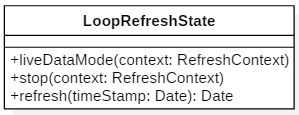
\includegraphics[width=0.5\linewidth]{images/view/classes/LoopRefreshState}
\end{figure} 
\subsubsection{Declaration}{
\begin{lstlisting}[frame=none]
public class LoopRefreshState
 extends View.TimeOption.RefreshState\end{lstlisting}
\subsubsection{Constructor summary}{
\begin{verse}
\hyperlink{View.TimeOption.LoopRefreshState()}{{\bf LoopRefreshState()}} Default constructor\\
\end{verse}
}
\subsubsection{Method summary}{
\begin{verse}
\hyperlink{View.TimeOption.LoopRefreshState.liveDataMode(View.TimeOption.RefreshContext)}{{\bf liveDataMode(RefreshContext)}} Switch to live data mode.\\
\hyperlink{View.TimeOption.LoopRefreshState.refresh(java.util.Date)}{{\bf refresh(Date)}} Returns the submitted time stamp modified according to the RefreshConfiguration.\\
\hyperlink{View.TimeOption.LoopRefreshState.stopRoutine(View.TimeOption.RefreshContext)}{{\bf stopRoutine(RefreshContext)}} Switch to historical mode.\\
\end{verse}
}
\subsubsection{Constructors}{
\vskip -2em
\begin{itemize}
\item{ 
\index{LoopRefreshState()}
\hypertarget{View.TimeOption.LoopRefreshState()}{{\bf  LoopRefreshState}\\}
\begin{lstlisting}[frame=none]
public LoopRefreshState()\end{lstlisting} %end signature
\begin{itemize}
\item{
{\bf  Description}

Default constructor
}
\end{itemize}
}%end item
\end{itemize}
}
\subsubsection{Methods}{
\vskip -2em
\begin{itemize}
\item{ 
\index{liveDataMode(RefreshContext)}
\hypertarget{View.TimeOption.LoopRefreshState.liveDataMode(View.TimeOption.RefreshContext)}{{\bf  liveDataMode}\\}
\begin{lstlisting}[frame=none]
public void liveDataMode(RefreshContext context)\end{lstlisting} %end signature
\begin{itemize}
\item{
{\bf  Description}

Switch to live data mode.
}
\item{
{\bf  Parameters}
  \begin{itemize}
   \item{
\texttt{context} -- }
  \end{itemize}
}%end item
\end{itemize}
}%end item
\item{ 
\index{refresh(Date)}
\hypertarget{View.TimeOption.LoopRefreshState.refresh(java.util.Date)}{{\bf  refresh}\\}
\begin{lstlisting}[frame=none]
public java.util.Date refresh(java.util.Date timeStamp)\end{lstlisting} %end signature
\begin{itemize}
\item{
{\bf  Description}

Returns the submitted time stamp modified according to the RefreshConfiguration.
}
\item{
{\bf  Parameters}
  \begin{itemize}
   \item{
\texttt{timeStamp} -- }
  \end{itemize}
}%end item
\item{{\bf  Returns} -- 
the submitted time stamp modified according to the RefreshConfiguration. 
}%end item
\end{itemize}
}%end item
\item{ 
\index{stopRoutine(RefreshContext)}
\hypertarget{View.TimeOption.LoopRefreshState.stopRoutine(View.TimeOption.RefreshContext)}{{\bf  stopRoutine}\\}
\begin{lstlisting}[frame=none]
public void stopRoutine(RefreshContext context)\end{lstlisting} %end signature
\begin{itemize}
\item{
{\bf  Description}

Switch to historical mode.
}
\item{
{\bf  Parameters}
  \begin{itemize}
   \item{
\texttt{context} -- }
  \end{itemize}
}%end item
\end{itemize}
}%end item
\end{itemize}
}
\subsubsection{Members inherited from class RefreshState }{
\texttt{View.TimeOption.RefreshState} {\small 
\refdefined{View.TimeOption.RefreshState}}
{\small 

\vskip -2em
\begin{itemize}
\item{\vskip -1.5ex 
\texttt{public void {\bf  continueRoutine}(\texttt{RefreshContext} {\bf  context})
}%end signature
}%end item
\item{\vskip -1.5ex 
\texttt{public void {\bf  historicalDataMode}(\texttt{RefreshContext} {\bf  context})
}%end signature
}%end item
\item{\vskip -1.5ex 
\texttt{public void {\bf  liveDataMode}(\texttt{RefreshContext} {\bf  context})
}%end signature
}%end item
\item{\vskip -1.5ex 
\texttt{public Date {\bf  refresh}(\texttt{java.util.Date} {\bf  timeStamp})
}%end signature
}%end item
\item{\vskip -1.5ex 
\texttt{public void {\bf  stopRoutine}(\texttt{RefreshContext} {\bf  context})
}%end signature
}%end item
\end{itemize}
}
}
\subsection{\label{View.TimeOption.RefreshConfiguration}Class RefreshConfiguration}{
\hypertarget{View.TimeOption.RefreshConfiguration}{}\vskip .1in 
Encapsulates the preferences about the fetching of live data and the loop mode of historical data.\vskip .1in
\begin{figure}[!hbp]
	\centering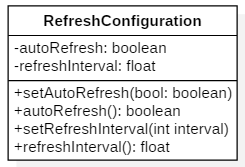
\includegraphics[width=0.5\linewidth]{images/view/classes/RefreshConfiguration}
\end{figure}  
\subsubsection{Declaration}{
\begin{lstlisting}[frame=none]
public class RefreshConfiguration
 extends java.lang.Object\end{lstlisting}
\subsubsection{Constructor summary}{
\begin{verse}
\hyperlink{View.TimeOption.RefreshConfiguration()}{{\bf RefreshConfiguration()}} Default constructor\\
\end{verse}
}
\subsubsection{Method summary}{
\begin{verse}
\hyperlink{View.TimeOption.RefreshConfiguration.autoRefresh()}{{\bf autoRefresh()}} In live mode return whether data should be fetched automatically or manually.\\
\hyperlink{View.TimeOption.RefreshConfiguration.refreshInterval()}{{\bf refreshInterval()}} Returns the interval in which automatic refreshes are made.\\
\hyperlink{View.TimeOption.RefreshConfiguration.setAutoRefresh(boolean)}{{\bf setAutoRefresh(boolean)}} In live mode set whether data should be fetched automatically or manually.\\
\hyperlink{View.TimeOption.RefreshConfiguration.setRefreshInterval(Interval)}{{\bf setRefreshInterval(Interval)}} Set the interval in which automatic refreshes are made.\\
\end{verse}
}
\subsubsection{Constructors}{
\vskip -2em
\begin{itemize}
\item{ 
\index{RefreshConfiguration()}
\hypertarget{View.TimeOption.RefreshConfiguration()}{{\bf  RefreshConfiguration}\\}
\begin{lstlisting}[frame=none]
public RefreshConfiguration()\end{lstlisting} %end signature
\begin{itemize}
\item{
{\bf  Description}

Default constructor
}
\end{itemize}
}%end item
\end{itemize}
}
\subsubsection{Methods}{
\vskip -2em
\begin{itemize}
\item{ 
\index{autoRefresh()}
\hypertarget{View.TimeOption.RefreshConfiguration.autoRefresh()}{{\bf  autoRefresh}\\}
\begin{lstlisting}[frame=none]
public boolean autoRefresh()\end{lstlisting} %end signature
\begin{itemize}
\item{
{\bf  Description}

In live mode return whether data should be fetched automatically or manually. In historic mode return whether in loop mode the time stamp should be refreshed automatically or manually.
}
\item{{\bf  Returns} -- 
in live mode whether data should be fetched automatically or manually and In historic mode whether in loop mode the time stamp should be refreshed automatically or manually. 
}%end item
\end{itemize}
}%end item
\item{ 
\index{refreshInterval()}
\hypertarget{View.TimeOption.RefreshConfiguration.refreshInterval()}{{\bf  refreshInterval}\\}
\begin{lstlisting}[frame=none]
public float refreshInterval()\end{lstlisting} %end signature
\begin{itemize}
\item{
{\bf  Description}

Returns the interval in which automatic refreshes are made.
}
\item{{\bf  Returns} -- 
the interval in which automatic refreshes are made. 
}%end item
\end{itemize}
}%end item
\item{ 
\index{setAutoRefresh(boolean)}
\hypertarget{View.TimeOption.RefreshConfiguration.setAutoRefresh(boolean)}{{\bf  setAutoRefresh}\\}
\begin{lstlisting}[frame=none]
public void setAutoRefresh(boolean bool)\end{lstlisting} %end signature
\begin{itemize}
\item{
{\bf  Description}

In live mode set whether data should be fetched automatically or manually. In historic mode set whether in loop mode the time stamp should be refreshed automatically or manually.
}
\item{
{\bf  Parameters}
  \begin{itemize}
   \item{
\texttt{bool} -- }
  \end{itemize}
}%end item
\end{itemize}
}%end item
\item{ 
\index{setRefreshInterval(Interval)}
\hypertarget{View.TimeOption.RefreshConfiguration.setRefreshInterval(Interval)}{{\bf  setRefreshInterval}\\}
\begin{lstlisting}[frame=none]
public void setRefreshInterval(Interval inv)\end{lstlisting} %end signature
\begin{itemize}
\item{
{\bf  Description}

Set the interval in which automatic refreshes are made.
}
\item{
{\bf  Parameters}
  \begin{itemize}
   \item{
\texttt{inv} -- }
  \end{itemize}
}%end item
\end{itemize}
}%end item
\end{itemize}
}
}
\subsection{\label{View.TimeOption.RefreshContext}Class RefreshContext}{
\hypertarget{View.TimeOption.RefreshContext}{}\vskip .1in 
Encapsulates the logic of switching between historical and live data mode and starting and stopping the loop mode. Through LiveRefreshConfiguration it also encapsulates whether live data is fetched automatically or manually and in which interval.\vskip .1in 
\begin{figure}[!hbp]
	\centering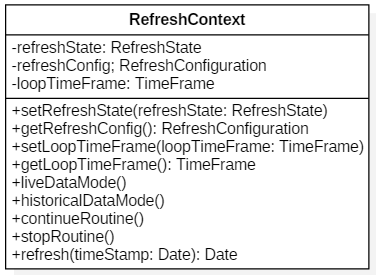
\includegraphics[width=0.5\linewidth]{images/view/classes/RefreshContext}
\end{figure} 
\subsubsection{Declaration}{
\begin{lstlisting}[frame=none]
public class RefreshContext
 extends java.lang.Object implements TimeOptionPanelObserver\end{lstlisting}
\subsubsection{Constructor summary}{
\begin{verse}
\hyperlink{View.TimeOption.RefreshContext()}{{\bf RefreshContext()}} Default constructor\\
\end{verse}
}
\subsubsection{Method summary}{
\begin{verse}
\hyperlink{View.TimeOption.RefreshContext.continueRoutine()}{{\bf continueRoutine()}} Continue the current routine.\\
\hyperlink{View.TimeOption.RefreshContext.getLoopTimeFrame()}{{\bf getLoopTimeFrame()}} Get the loop time frame.\\
\hyperlink{View.TimeOption.RefreshContext.getRefreshConfig()}{{\bf getRefreshConfig()}} Get the RefreshConfiguration.\\
\hyperlink{View.TimeOption.RefreshContext.historicalDataMode()}{{\bf historicalDataMode()}} Switch to historical data mode.\\
\hyperlink{View.TimeOption.RefreshContext.liveDataMode()}{{\bf liveDataMode()}} Switch to live data mode.\\
\hyperlink{View.TimeOption.RefreshContext.refresh(java.util.Date)}{{\bf refresh(Date)}} Refresh the submitted time stamp depending on the TimeStampState by returning a new time stamp.\\
\hyperlink{View.TimeOption.RefreshContext.setLoopTimeFrame(TimeFrame)}{{\bf setLoopTimeFrame(TimeFrame)}} Set the start and end time point of the loop.\\
\hyperlink{View.TimeOption.RefreshContext.setRefreshState(View.TimeOption.RefreshState)}{{\bf setRefreshState(RefreshState)}} Set the current refresh state.\\
\hyperlink{View.TimeOption.RefreshContext.stopRoutine()}{{\bf stopRoutine()}} Stop the current routine.\\
\hyperlink{View.TimeOption.RefreshContext.timeOptionUpdate()}{{\bf timeOptionUpdate()}} Update the observer with the current TimeOptionPanel state.\\
\end{verse}
}
\subsubsection{Constructors}{
\vskip -2em
\begin{itemize}
\item{ 
\index{RefreshContext()}
\hypertarget{View.TimeOption.RefreshContext()}{{\bf  RefreshContext}\\}
\begin{lstlisting}[frame=none]
public RefreshContext()\end{lstlisting} %end signature
\begin{itemize}
\item{
{\bf  Description}

Default constructor
}
\end{itemize}
}%end item
\end{itemize}
}
\subsubsection{Methods}{
\vskip -2em
\begin{itemize}
\item{ 
\index{continueRoutine()}
\hypertarget{View.TimeOption.RefreshContext.continueRoutine()}{{\bf  continueRoutine}\\}
\begin{lstlisting}[frame=none]
public void continueRoutine()\end{lstlisting} %end signature
\begin{itemize}
\item{
{\bf  Description}

Continue the current routine.
}
\end{itemize}
}%end item
\item{ 
\index{getLoopTimeFrame()}
\hypertarget{View.TimeOption.RefreshContext.getLoopTimeFrame()}{{\bf  getLoopTimeFrame}\\}
\begin{lstlisting}[frame=none]
public TimeFrame getLoopTimeFrame()\end{lstlisting} %end signature
\begin{itemize}
\item{
{\bf  Description}

Get the loop time frame.
}
\item{{\bf  Returns} -- 
the loop time frame. 
}%end item
\end{itemize}
}%end item
\item{ 
\index{getRefreshConfig()}
\hypertarget{View.TimeOption.RefreshContext.getRefreshConfig()}{{\bf  getRefreshConfig}\\}
\begin{lstlisting}[frame=none]
public RefreshConfiguration getRefreshConfig()\end{lstlisting} %end signature
\begin{itemize}
\item{
{\bf  Description}

Get the RefreshConfiguration.
}
\item{{\bf  Returns} -- 
the RefreshConfiguration. 
}%end item
\end{itemize}
}%end item
\item{ 
\index{historicalDataMode()}
\hypertarget{View.TimeOption.RefreshContext.historicalDataMode()}{{\bf  historicalDataMode}\\}
\begin{lstlisting}[frame=none]
public void historicalDataMode()\end{lstlisting} %end signature
\begin{itemize}
\item{
{\bf  Description}

Switch to historical data mode.
}
\end{itemize}
}%end item
\item{ 
\index{liveDataMode()}
\hypertarget{View.TimeOption.RefreshContext.liveDataMode()}{{\bf  liveDataMode}\\}
\begin{lstlisting}[frame=none]
public void liveDataMode()\end{lstlisting} %end signature
\begin{itemize}
\item{
{\bf  Description}

Switch to live data mode.
}
\end{itemize}
}%end item
\item{ 
\index{refresh(Date)}
\hypertarget{View.TimeOption.RefreshContext.refresh(java.util.Date)}{{\bf  refresh}\\}
\begin{lstlisting}[frame=none]
public java.util.Date refresh(java.util.Date timeStamp)\end{lstlisting} %end signature
\begin{itemize}
\item{
{\bf  Description}

Refresh the submitted time stamp depending on the TimeStampState by returning a new time stamp.
}
\item{
{\bf  Parameters}
  \begin{itemize}
   \item{
\texttt{timeStamp} -- }
  \end{itemize}
}%end item
\item{{\bf  Returns} -- 
the submitted time stamp altered depending on the TimeStampState. 
}%end item
\end{itemize}
}%end item
\item{ 
\index{setLoopTimeFrame(TimeFrame)}
\hypertarget{View.TimeOption.RefreshContext.setLoopTimeFrame(TimeFrame)}{{\bf  setLoopTimeFrame}\\}
\begin{lstlisting}[frame=none]
public void setLoopTimeFrame(TimeFrame loopTimeFrame)\end{lstlisting} %end signature
\begin{itemize}
\item{
{\bf  Description}

Set the start and end time point of the loop.
}
\item{
{\bf  Parameters}
  \begin{itemize}
   \item{
\texttt{loopTimeFrame} -- }
  \end{itemize}
}%end item
\end{itemize}
}%end item
\item{ 
\index{setRefreshState(RefreshState)}
\hypertarget{View.TimeOption.RefreshContext.setRefreshState(View.TimeOption.RefreshState)}{{\bf  setRefreshState}\\}
\begin{lstlisting}[frame=none]
public void setRefreshState(RefreshState refreshState)\end{lstlisting} %end signature
\begin{itemize}
\item{
{\bf  Description}

Set the current refresh state.
}
\item{
{\bf  Parameters}
  \begin{itemize}
   \item{
\texttt{refreshState} -- }
  \end{itemize}
}%end item
\end{itemize}
}%end item
\item{ 
\index{stopRoutine()}
\hypertarget{View.TimeOption.RefreshContext.stopRoutine()}{{\bf  stopRoutine}\\}
\begin{lstlisting}[frame=none]
public void stopRoutine()\end{lstlisting} %end signature
\begin{itemize}
\item{
{\bf  Description}

Stop the current routine.
}
\end{itemize}
}%end item
\item{ 
\index{timeOptionUpdate()}
\hypertarget{View.TimeOption.RefreshContext.timeOptionUpdate()}{{\bf  timeOptionUpdate}\\}
\begin{lstlisting}[frame=none]
public void timeOptionUpdate()\end{lstlisting} %end signature
\begin{itemize}
\item{
{\bf  Description}

Update the observer with the current TimeOptionPanel state.
}
\end{itemize}
}%end item
\end{itemize}
}
}
\subsection{\label{View.TimeOption.RefreshState}Class RefreshState}{
\hypertarget{View.TimeOption.RefreshState}{}\vskip .1in 
Encapsulates behaviour concerning refreshing time stamps and dealing with historical and live data fetching.\vskip .1in 
\begin{figure}[!hbp]
	\centering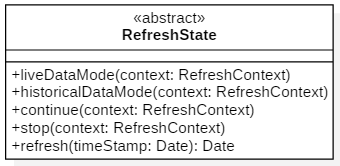
\includegraphics[width=0.5\linewidth]{images/view/classes/RefreshState}
\end{figure} 
\subsubsection{Declaration}{
\begin{lstlisting}[frame=none]
public class RefreshState
 extends java.lang.Object\end{lstlisting}
\subsubsection{All known subclasses}{LoopRefreshState\small{\refdefined{View.TimeOption.LoopRefreshState}}, LiveRefreshState\small{\refdefined{View.TimeOption.LiveRefreshState}}, HistoricalRefreshState\small{\refdefined{View.TimeOption.HistoricalRefreshState}}}
\subsubsection{Constructor summary}{
\begin{verse}
\hyperlink{View.TimeOption.RefreshState()}{{\bf RefreshState()}} Default constructor\\
\end{verse}
}
\subsubsection{Method summary}{
\begin{verse}
\hyperlink{View.TimeOption.RefreshState.continueRoutine(View.TimeOption.RefreshContext)}{{\bf continueRoutine(RefreshContext)}} Continue the current routine.\\
\hyperlink{View.TimeOption.RefreshState.historicalDataMode(View.TimeOption.RefreshContext)}{{\bf historicalDataMode(RefreshContext)}} Switch to historical data mode.\\
\hyperlink{View.TimeOption.RefreshState.liveDataMode(View.TimeOption.RefreshContext)}{{\bf liveDataMode(RefreshContext)}} Switch to live data mode.\\
\hyperlink{View.TimeOption.RefreshState.refresh(java.util.Date)}{{\bf refresh(Date)}} Refresh the the submitted time stamp depending on the TimeStampState by returning a new time stamp.\\
\hyperlink{View.TimeOption.RefreshState.stopRoutine(View.TimeOption.RefreshContext)}{{\bf stopRoutine(RefreshContext)}} Stop the current routine.\\
\end{verse}
}
\subsubsection{Constructors}{
\vskip -2em
\begin{itemize}
\item{ 
\index{RefreshState()}
\hypertarget{View.TimeOption.RefreshState()}{{\bf  RefreshState}\\}
\begin{lstlisting}[frame=none]
public RefreshState()\end{lstlisting} %end signature
\begin{itemize}
\item{
{\bf  Description}

Default constructor
}
\end{itemize}
}%end item
\end{itemize}
}
\subsubsection{Methods}{
\vskip -2em
\begin{itemize}
\item{ 
\index{continueRoutine(RefreshContext)}
\hypertarget{View.TimeOption.RefreshState.continueRoutine(View.TimeOption.RefreshContext)}{{\bf  continueRoutine}\\}
\begin{lstlisting}[frame=none]
public void continueRoutine(RefreshContext context)\end{lstlisting} %end signature
\begin{itemize}
\item{
{\bf  Description}

Continue the current routine.
}
\item{
{\bf  Parameters}
  \begin{itemize}
   \item{
\texttt{context} -- }
  \end{itemize}
}%end item
\end{itemize}
}%end item
\item{ 
\index{historicalDataMode(RefreshContext)}
\hypertarget{View.TimeOption.RefreshState.historicalDataMode(View.TimeOption.RefreshContext)}{{\bf  historicalDataMode}\\}
\begin{lstlisting}[frame=none]
public void historicalDataMode(RefreshContext context)\end{lstlisting} %end signature
\begin{itemize}
\item{
{\bf  Description}

Switch to historical data mode.
}
\item{
{\bf  Parameters}
  \begin{itemize}
   \item{
\texttt{context} -- }
  \end{itemize}
}%end item
\end{itemize}
}%end item
\item{ 
\index{liveDataMode(RefreshContext)}
\hypertarget{View.TimeOption.RefreshState.liveDataMode(View.TimeOption.RefreshContext)}{{\bf  liveDataMode}\\}
\begin{lstlisting}[frame=none]
public void liveDataMode(RefreshContext context)\end{lstlisting} %end signature
\begin{itemize}
\item{
{\bf  Description}

Switch to live data mode.
}
\item{
{\bf  Parameters}
  \begin{itemize}
   \item{
\texttt{context} -- }
  \end{itemize}
}%end item
\end{itemize}
}%end item
\item{ 
\index{refresh(Date)}
\hypertarget{View.TimeOption.RefreshState.refresh(java.util.Date)}{{\bf  refresh}\\}
\begin{lstlisting}[frame=none]
public java.util.Date refresh(java.util.Date timeStamp)\end{lstlisting} %end signature
\begin{itemize}
\item{
{\bf  Description}

Refresh the the submitted time stamp depending on the TimeStampState by returning a new time stamp.
}
\item{
{\bf  Parameters}
  \begin{itemize}
   \item{
\texttt{timeStamp} -- }
  \end{itemize}
}%end item
\item{{\bf  Returns} -- 
the most up-to-date time stamp. 
}%end item
\end{itemize}
}%end item
\item{ 
\index{stopRoutine(RefreshContext)}
\hypertarget{View.TimeOption.RefreshState.stopRoutine(View.TimeOption.RefreshContext)}{{\bf  stopRoutine}\\}
\begin{lstlisting}[frame=none]
public void stopRoutine(RefreshContext context)\end{lstlisting} %end signature
\begin{itemize}
\item{
{\bf  Description}

Stop the current routine.
}
\item{
{\bf  Parameters}
  \begin{itemize}
   \item{
\texttt{context} -- }
  \end{itemize}
}%end item
\end{itemize}
}%end item
\end{itemize}
}
}
\subsection{\label{View.TimeOption.TimeOptionPanel}Class TimeOptionPanel}{
\hypertarget{View.TimeOption.TimeOptionPanel}{}\vskip .1in 
An implementation of AbstractTimeOptionPanel.\vskip .1in 
\begin{figure}[!hbp]
	\centering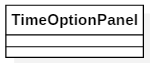
\includegraphics[width=0.5\linewidth]{images/view/classes/TimeOptionPanel}
\end{figure} 
\subsubsection{Declaration}{
\begin{lstlisting}[frame=none]
public class TimeOptionPanel
 extends View.TimeOption.AbstractTimeOptionPanel\end{lstlisting}
\subsubsection{Constructor summary}{
\begin{verse}
\hyperlink{View.TimeOption.TimeOptionPanel()}{{\bf TimeOptionPanel()}} Default constructor\\
\end{verse}
}
\subsubsection{Constructors}{
\vskip -2em
\begin{itemize}
\item{ 
\index{TimeOptionPanel()}
\hypertarget{View.TimeOption.TimeOptionPanel()}{{\bf  TimeOptionPanel}\\}
\begin{lstlisting}[frame=none]
public TimeOptionPanel()\end{lstlisting} %end signature
\begin{itemize}
\item{
{\bf  Description}

Default constructor
}
\end{itemize}
}%end item
\end{itemize}
}
\subsubsection{Members inherited from class AbstractTimeOptionPanel }{
\texttt{View.TimeOption.AbstractTimeOptionPanel} {\small 
\refdefined{View.TimeOption.AbstractTimeOptionPanel}}
{\small 

\vskip -2em
\begin{itemize}
\item{\vskip -1.5ex 
\texttt{public TimeFrame {\bf  getLoopTimeframe}()
}%end signature
}%end item
\item{\vskip -1.5ex 
\texttt{public RefreshContext {\bf  getRefreshContext}()
}%end signature
}%end item
\item{\vskip -1.5ex 
\texttt{public Date {\bf  getTimeStamp}()
}%end signature
}%end item
\item{\vskip -1.5ex 
\texttt{protected {\bf  loopTimeFrame}}%end signature
}%end item
\item{\vskip -1.5ex 
\texttt{public void {\bf  notify}()
}%end signature
}%end item
\item{\vskip -1.5ex 
\texttt{protected {\bf  refreshConfig}}%end signature
}%end item
\item{\vskip -1.5ex 
\texttt{public void {\bf  setLoopTimeFrame}(\texttt{TimeFrame} {\bf  loopTimeFrame})
}%end signature
}%end item
\item{\vskip -1.5ex 
\texttt{public void {\bf  setTimeStamp}(\texttt{java.util.Date} {\bf  timeStamp})
}%end signature
}%end item
\item{\vskip -1.5ex 
\texttt{public void {\bf  subscribeObserver}(\texttt{TimeOptionPanelObserver} {\bf  observer})
}%end signature
}%end item
\item{\vskip -1.5ex 
\texttt{protected {\bf  timeStamp}}%end signature
}%end item
\item{\vskip -1.5ex 
\texttt{public void {\bf  unsubscribeObserver}(\texttt{TimeOptionPanelObserver} {\bf  observer})
}%end signature
}%end item
\end{itemize}
}
}
}
\section{Package View.Util}{
\label{View.Util}\hypertarget{View.Util}{}
\hskip -.05in
\hbox to \hsize{\textit{ Package Contents\hfil Page}}
\vskip .13in
\hbox{{\bf  Classes}}
\entityintro{ClusterID}{View.Util.ClusterID}{A Cluster Identifier.}
\entityintro{Date}{View.Util.Date}{Represents a specific point in time.}
\entityintro{Identifier}{View.Util.Identifier}{Represents an identifier made up of a String.}
\entityintro{Point}{View.Util.Point}{A point representing a location in (x,y) coordinate space, specified in float precision.}
\entityintro{SensorID}{View.Util.SensorID}{A Sensor Identifier.}
\entityintro{TimeFrame}{View.Util.TimeFrame}{A period of time, specified by a start and end date.}
\vskip .1in
\vskip .1in
\subsection{\label{View.Util.ClusterID}Class ClusterID}{
\hypertarget{View.Util.ClusterID}{}\vskip .1in 
A Cluster Identifier.\vskip .1in 
\begin{figure}[!hbp]
	\centering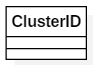
\includegraphics[width=0.5\linewidth]{images/view/classes/ClusterID}
\end{figure} 
\subsubsection{Declaration}{
\begin{lstlisting}[frame=none]
public class ClusterID
 extends View.Util.Identifier\end{lstlisting}
\subsubsection{Constructor summary}{
\begin{verse}
\hyperlink{View.Util.ClusterID()}{{\bf ClusterID()}} Default constructor\\
\end{verse}
}
\subsubsection{Constructors}{
\vskip -2em
\begin{itemize}
\item{ 
\index{ClusterID()}
\hypertarget{View.Util.ClusterID()}{{\bf  ClusterID}\\}
\begin{lstlisting}[frame=none]
public ClusterID()\end{lstlisting} %end signature
\begin{itemize}
\item{
{\bf  Description}

Default constructor
}
\end{itemize}
}%end item
\end{itemize}
}
\subsubsection{Members inherited from class Identifier }{
\texttt{View.Util.Identifier} {\small 
\refdefined{View.Util.Identifier}}
{\small 

\vskip -2em
\begin{itemize}
\item{\vskip -1.5ex 
\texttt{public boolean {\bf  equals}(\texttt{Identifier} {\bf  other})
}%end signature
}%end item
\end{itemize}
}
}
\subsection{\label{View.Util.Date}Class Date}{
\hypertarget{View.Util.Date}{}\vskip .1in 
Represents a specific point in time.\vskip .1in 
\begin{figure}[!hbp]
	\centering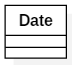
\includegraphics[width=0.5\linewidth]{images/view/classes/Date}
\end{figure} 
\subsubsection{Declaration}{
\begin{lstlisting}[frame=none]
public class Date
 extends java.lang.Object\end{lstlisting}
\subsubsection{Constructor summary}{
\begin{verse}
\hyperlink{View.Util.Date()}{{\bf Date()}} Default constructor\\
\end{verse}
}
\subsubsection{Constructors}{
\vskip -2em
\begin{itemize}
\item{ 
\index{Date()}
\hypertarget{View.Util.Date()}{{\bf  Date}\\}
\begin{lstlisting}[frame=none]
public Date()\end{lstlisting} %end signature
\begin{itemize}
\item{
{\bf  Description}

Default constructor
}
\end{itemize}
}%end item
\end{itemize}
}
}
\subsection{\label{View.Util.Identifier}Class Identifier}{
\hypertarget{View.Util.Identifier}{}\vskip .1in 
Represents an identifier made up of a String.\vskip .1in 
\begin{figure}[!hbp]
	\centering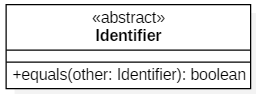
\includegraphics[width=0.5\linewidth]{images/view/classes/Identifier}
\end{figure} 
\subsubsection{Declaration}{
\begin{lstlisting}[frame=none]
public class Identifier
 extends java.lang.Object\end{lstlisting}
\subsubsection{All known subclasses}{SensorID\small{\refdefined{View.Util.SensorID}}, ClusterID\small{\refdefined{View.Util.ClusterID}}}
\subsubsection{Constructor summary}{
\begin{verse}
\hyperlink{View.Util.Identifier()}{{\bf Identifier()}} Default constructor\\
\end{verse}
}
\subsubsection{Method summary}{
\begin{verse}
\hyperlink{View.Util.Identifier.equals(View.Util.Identifier)}{{\bf equals(Identifier)}} Returns whether this identifier is equal to the submitted identifier or not.\\
\end{verse}
}
\subsubsection{Constructors}{
\vskip -2em
\begin{itemize}
\item{ 
\index{Identifier()}
\hypertarget{View.Util.Identifier()}{{\bf  Identifier}\\}
\begin{lstlisting}[frame=none]
public Identifier()\end{lstlisting} %end signature
\begin{itemize}
\item{
{\bf  Description}

Default constructor
}
\end{itemize}
}%end item
\end{itemize}
}
\subsubsection{Methods}{
\vskip -2em
\begin{itemize}
\item{ 
\index{equals(Identifier)}
\hypertarget{View.Util.Identifier.equals(View.Util.Identifier)}{{\bf  equals}\\}
\begin{lstlisting}[frame=none]
public boolean equals(Identifier other)\end{lstlisting} %end signature
\begin{itemize}
\item{
{\bf  Description}

Returns whether this identifier is equal to the submitted identifier or not.
}
\item{
{\bf  Parameters}
  \begin{itemize}
   \item{
\texttt{other} -- }
  \end{itemize}
}%end item
\item{{\bf  Returns} -- 
 
}%end item
\end{itemize}
}%end item
\end{itemize}
}
}
\subsection{\label{View.Util.Point}Class Point}{
\hypertarget{View.Util.Point}{}\vskip .1in 
A point representing a location in (x,y) coordinate space, specified in float precision.\vskip .1in 
\begin{figure}[!hbp]
	\centering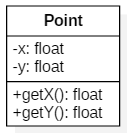
\includegraphics[width=0.5\linewidth]{images/view/classes/Point}
\end{figure} 
\subsubsection{Declaration}{
\begin{lstlisting}[frame=none]
public class Point
 extends java.lang.Object\end{lstlisting}
\subsubsection{Constructor summary}{
\begin{verse}
\hyperlink{View.Util.Point()}{{\bf Point()}} Default constructor\\
\end{verse}
}
\subsubsection{Method summary}{
\begin{verse}
\hyperlink{View.Util.Point.getX()}{{\bf getX()}} Returns the x coordinate of this point.\\
\hyperlink{View.Util.Point.getY()}{{\bf getY()}} Returns the y coordinate of this point.\\
\end{verse}
}
\subsubsection{Constructors}{
\vskip -2em
\begin{itemize}
\item{ 
\index{Point()}
\hypertarget{View.Util.Point()}{{\bf  Point}\\}
\begin{lstlisting}[frame=none]
public Point()\end{lstlisting} %end signature
\begin{itemize}
\item{
{\bf  Description}

Default constructor
}
\end{itemize}
}%end item
\end{itemize}
}
\subsubsection{Methods}{
\vskip -2em
\begin{itemize}
\item{ 
\index{getX()}
\hypertarget{View.Util.Point.getX()}{{\bf  getX}\\}
\begin{lstlisting}[frame=none]
public float getX()\end{lstlisting} %end signature
\begin{itemize}
\item{
{\bf  Description}

Returns the x coordinate of this point.
}
\item{{\bf  Returns} -- 
 
}%end item
\end{itemize}
}%end item
\item{ 
\index{getY()}
\hypertarget{View.Util.Point.getY()}{{\bf  getY}\\}
\begin{lstlisting}[frame=none]
public float getY()\end{lstlisting} %end signature
\begin{itemize}
\item{
{\bf  Description}

Returns the y coordinate of this point.
}
\item{{\bf  Returns} -- 
 
}%end item
\end{itemize}
}%end item
\end{itemize}
}
}
\subsection{\label{View.Util.SensorID}Class SensorID}{
\hypertarget{View.Util.SensorID}{}\vskip .1in 
A Sensor Identifier.\vskip .1in 
\begin{figure}[!hbp]
	\centering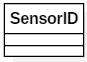
\includegraphics[width=0.5\linewidth]{images/view/classes/SensorID}
\end{figure} 
\subsubsection{Declaration}{
\begin{lstlisting}[frame=none]
public class SensorID
 extends View.Util.Identifier\end{lstlisting}
\subsubsection{Constructor summary}{
\begin{verse}
\hyperlink{View.Util.SensorID()}{{\bf SensorID()}} Default constructor\\
\end{verse}
}
\subsubsection{Constructors}{
\vskip -2em
\begin{itemize}
\item{ 
\index{SensorID()}
\hypertarget{View.Util.SensorID()}{{\bf  SensorID}\\}
\begin{lstlisting}[frame=none]
public SensorID()\end{lstlisting} %end signature
\begin{itemize}
\item{
{\bf  Description}

Default constructor
}
\end{itemize}
}%end item
\end{itemize}
}
\subsubsection{Members inherited from class Identifier }{
\texttt{View.Util.Identifier} {\small 
\refdefined{View.Util.Identifier}}
{\small 

\vskip -2em
\begin{itemize}
\item{\vskip -1.5ex 
\texttt{public boolean {\bf  equals}(\texttt{Identifier} {\bf  other})
}%end signature
}%end item
\end{itemize}
}
}
\subsection{\label{View.Util.TimeFrame}Class TimeFrame}{
\hypertarget{View.Util.TimeFrame}{}\vskip .1in 
A period of time, specified by a start and end date.\vskip .1in 
\begin{figure}[!hbp]
	\centering\includegraphics[width=0.5\linewidth]{images/view/classes/TimeFrame}
\end{figure} 
\subsubsection{Declaration}{
\begin{lstlisting}[frame=none]
public class TimeFrame
 extends java.lang.Object\end{lstlisting}
\subsubsection{Constructor summary}{
\begin{verse}
\hyperlink{View.Util.TimeFrame()}{{\bf TimeFrame()}} Default constructor\\
\end{verse}
}
\subsubsection{Method summary}{
\begin{verse}
\hyperlink{View.Util.TimeFrame.getEnd()}{{\bf getEnd()}} Returns the end date of this time frame.\\
\hyperlink{View.Util.TimeFrame.getStart()}{{\bf getStart()}} Returns the start date of this time frame.\\
\end{verse}
}
\subsubsection{Constructors}{
\vskip -2em
\begin{itemize}
\item{ 
\index{TimeFrame()}
\hypertarget{View.Util.TimeFrame()}{{\bf  TimeFrame}\\}
\begin{lstlisting}[frame=none]
public TimeFrame()\end{lstlisting} %end signature
\begin{itemize}
\item{
{\bf  Description}

Default constructor
}
\end{itemize}
}%end item
\end{itemize}
}
\subsubsection{Methods}{
\vskip -2em
\begin{itemize}
\item{ 
\index{getEnd()}
\hypertarget{View.Util.TimeFrame.getEnd()}{{\bf  getEnd}\\}
\begin{lstlisting}[frame=none]
public Date getEnd()\end{lstlisting} %end signature
\begin{itemize}
\item{
{\bf  Description}

Returns the end date of this time frame.
}
\item{{\bf  Returns} -- 
 
}%end item
\end{itemize}
}%end item
\item{ 
\index{getStart()}
\hypertarget{View.Util.TimeFrame.getStart()}{{\bf  getStart}\\}
\begin{lstlisting}[frame=none]
public Date getStart()\end{lstlisting} %end signature
\begin{itemize}
\item{
{\bf  Description}

Returns the start date of this time frame.
}
\item{{\bf  Returns} -- 
 
}%end item
\end{itemize}
}%end item
\end{itemize}
}
}
}
